\documentclass[dvipdfmx]{OFbook}
\setcounter{secnumdepth}{4}
\nofiles

\usepackage{color}
\usepackage{graphicx}
\graphicspath{{./fig/pdf/}{./fig/png/}}
\usepackage{ltxtable}

\usepackage[deluxe,uplatex,jis2004]{otf}
\usepackage{lmodern}
\usepackage[T1]{fontenc}
\usepackage{textcomp}
\usepackage[utf8]{inputenc}
\usepackage{amsmath,amssymb}
\usepackage{bm}

\usepackage[
 bookmarks=true,
 bookmarksnumbered=true,
 pdftitle={OpenFOAM Programmer's Guide},
 pdfsubject={Japanese edition},
 pdfauthor={The Open CAE Society of Japan (www.opencae.jp)},
 pdfkeywords={OpenFOAM},
 colorlinks=true,
 linkcolor=red,
 filecolor=blue,
 urlcolor=blue
 ]{hyperref}[2007/12/08]
\usepackage{pxjahyper}

\usepackage{OFmacros}

\usepackage{makeidx}
\makeindex
\def\seename{$\Longrightarrow$}

\title{プログラマズガイド和訳}
\author{一般社団法人 オープンCAE学会}
\version{2.3.0}
\def\thepage{P-\arabic{page}}

\begin{document}

\maketitle
\frontmatter

\begin{OFdeclaration}
 %#! uplatex UserGuideJa

Copyright \copyright{} 2006--2016 一般社団法人 オープンCAE学会

\vskip\Cvs

このユーザガイド和訳は,
一般社団法人 オープンCAE学会の責任のもとで公開しております.
本書に関するご意見等がございましたら,
当学会事務局 (\href{mailto:office@opencae.jp}{office@opencae.jp}) までご連絡ください.

\vskip2\Cvs

次ページ以降に示すとおり,このユーザガイドは
クリエイティブ・コモンズ「表示・非営利・改変禁止3.0非移植」(CC BY-NC-ND 3.0) ライセンス
となっています.
当学会は,権利者であるOpenFOAM Foundationより翻訳・再配布の許諾を得ています.

\vskip\Cvs

\hfill 一般社団法人 オープンCAE学会\par

\vskip\Cvs

\noindent
Typeset in p\LaTeX.


\chapter{原文著作権表示}
Copyright \copyright{} 2011--2015 OpenFOAM Foundation Ltd.\par
Author: Christopher J. Greenshields, CFD Direct Ltd.

\vskip\Cvs

This work is licensed under a
\textbf{Creative Commons Attribution-NonCommercial-NoDerivs 3.0 Unported License}.

\vskip\Cvs

%#! uplatex UserGuideJa

\section*{License}
THE WORK (AS DEFINED BELOW) IS PROVIDED UNDER THE TERMS OF THIS CREATIVE COMMONS PUBLIC LICENSE
(``CCPL'' OR ``LICENSE'').
THE WORK IS PROTECTED BY COPYRIGHT AND/OR OTHER APPLICABLE LAW.
ANY USE OF THE WORK OTHER THAN AS AUTHORIZED UNDER THIS LICENSE OR COPYRIGHT LAW IS PROHIBITED.
BY EXERCISING ANY RIGHTS TO THE WORK PROVIDED HERE,
YOU ACCEPT AND AGREE TO BE BOUND BY THE TERMS OF THIS LICENSE.
TO THE EXTENT THIS LICENSE MAY BE CONSIDERED TO BE A CONTRACT,
THE LICENSOR GRANTS YOU THE RIGHTS CONTAINED HERE IN CONSIDERATION OF
YOUR ACCEPTANCE OF SUCH TERMS AND CONDITIONS.


\section{Definitions}
\begin{enumerate}
 \item  ``Adaptation'' means a work based upon the Work, or upon the
        Work and other preexisting works, such as a translation,
        adaptation, derivative work, arrangement of music or other
        alterations of a literary or artistic work, or phonogram or
        performance and includes cinematographic adaptations or any
        other form in which the Work may be recast, transformed, or
        adapted including in any form recognizably derived from the
        original, except that a work that constitutes a Collection will
        not be considered an Adaptation for the purpose of this
        License. For the avoidance of doubt, where the Work is a musical
        work, performance or phonogram, the synchronization of the Work
        in timed-relation with a moving image (``synching'') will be
        considered an Adaptation for the purpose of this License.
 \item ``Collection'' means a collection of literary or artistic works,
       such as encyclopedias and anthologies, or performances,
       phonograms or broadcasts, or other works or subject matter other
       than works listed in Section 1(f) below, which, by reason of the
       selection and arrangement of their contents, constitute
       intellectual creations, in which the Work is included in its
       entirety in unmodified form along with one or more other
       contributions, each constituting separate and independent works
       in themselves, which together are assembled into a collective
       whole. A work that constitutes a Collection will not be
       considered an Adaptation (as defined above) for the purposes of
       this License.
 \item ``Distribute'' means to make available to the public the original
       and copies of the Work through sale or other transfer of
       ownership.
 \item ``Licensor'' means the individual, individuals, entity or
       entities that offer(s) the Work under the terms of this License.
 \item ``Original Author'' means, in the case of a literary or artistic
       work, the individual, individuals, entity or entities who created
       the Work or if no individual or entity can be identified, the
       publisher; and in addition (i) in the case of a performance the
       actors, singers, musicians, dancers, and other persons who act,
       sing, deliver, declaim, play in, interpret or otherwise perform
       literary or artistic works or expressions of folklore; (ii) in
       the case of a phonogram the producer being the person or legal
       entity who first fixes the sounds of a performance or other
       sounds; and, (iii) in the case of broadcasts, the organization
       that transmits the broadcast.
 \item ``Work'' means the literary and/or artistic work offered under
       the terms of this License including without limitation any
       production in the literary, scientific and artistic domain,
       whatever may be the mode or form of its expression including
       digital form, such as a book, pamphlet and other writing; a
       lecture, address, sermon or other work of the same nature; a
       dramatic or dramatico-musical work; a choreographic work or
       entertainment in dumb show; a musical composition with or without
       words; a cinematographic work to which are assimilated works
       expressed by a process analogous to cinematography; a work of
       drawing, painting, architecture, sculpture, engraving or
       lithography; a photographic work to which are assimilated works
       expressed by a process analogous to photography; a work of
       applied art; an illustration, map, plan, sketch or
       three-dimensional work relative to geography, topography,
       architecture or science; a performance; a broadcast; a phonogram;
       a compilation of data to the extent it is protected as a
       copyrightable work; or a work performed by a variety or circus
       performer to the extent it is not otherwise considered a literary
       or artistic work.
 \item ``You'' means an individual or entity exercising rights under
       this License who has not previously violated the terms of this
       License with respect to the Work, or who has received express
       permission from the Licensor to exercise rights under this
       License despite a previous violation.
 \item ``Publicly Perform'' means to perform public recitations of the
       Work and to communicate to the public those public recitations,
       by any means or process, including by wire or wireless means or
       public digital performances; to make available to the public
       Works in such a way that members of the public may access these
       Works from a place and at a place individually chosen by them; to
       perform the Work to the public by any means or process and the
       communication to the public of the performances of the Work,
       including by public digital performance; to broadcast and
       rebroadcast the Work by any means including signs, sounds or
       images.
 \item ``Reproduce'' means to make copies of the Work by any means
       including without limitation by sound or visual recordings and
       the right of fixation and reproducing fixations of the Work,
       including storage of a protected performance or phonogram in
       digital form or other electronic medium.
\end{enumerate}


\section{Fair Dealing Rights.}
Nothing in this License is intended to reduce, limit, or restrict any
uses free from copyright or rights arising from limitations or
exceptions that are provided for in connection with the copyright
protection under copyright law or other applicable laws.


\section{License Grant.}
Subject to the terms and conditions of this License, Licensor hereby
grants You a worldwide, royalty-free, non-exclusive, perpetual (for the
duration of the applicable copyright) license to exercise the rights in
the Work as stated below:
\begin{enumerate}
 \item to Reproduce the Work, to incorporate the
       Work into one or more Collections, and to Reproduce the Work as
       incorporated in the Collections;
 \item and, to Distribute and Publicly
       Perform the Work including as incorporated in Collections. The
       above rights may be exercised in all media and formats whether
       now known or hereafter devised.
\end{enumerate}
The above rights include the right to make such modifications as are
technically necessary to exercise the rights in other media and formats,
but otherwise you have no rights to make Adaptations. Subject to 8(f),
all rights not expressly granted by Licensor are hereby reserved,
including but not limited to the rights set forth in Section 4(d).


\section{Restrictions.}
The license granted in Section 3 above is expressly made subject to and
limited by the following restrictions:

\begin{enumerate}
 \item You may Distribute or Publicly Perform the Work only under the
       terms of this License. You must include a copy of, or the Uniform
       Resource Identifier (URI) for, this License  with every copy of
       the Work You Distribute or Publicly Perform. You may not offer or
       impose any terms on the Work that restrict the terms of this
       License or the ability of the recipient of the Work to exercise
       the rights granted to that recipient under the terms of the
       License. You may not sublicense the Work. You must keep intact
       all notices that refer to this License and to the disclaimer of
       warranties with every copy of the Work You Distribute or Publicly
       Perform. When You Distribute or Publicly Perform the Work, You
       may not impose any effective technological measures on the Work
       that restrict the ability of a recipient of the Work from You to
       exercise the rights granted to that recipient under the terms of
       the License. This Section 4(a) applies to the Work as
       incorporated in a Collection, but this does not require the
       Collection apart from the Work itself to be made subject to the
       terms of this License. If You create a Collection, upon notice
       from any Licensor You must, to the extent practicable, remove
       from the Collection any credit as required by Section 4(c), as
       requested.
 \item You may not exercise any of the rights granted to You in Section
       3 above in any manner that is primarily intended for or directed
       toward commercial advantage or private monetary compensation. The
       exchange of the Work for other copyrighted works by means of
       digital file-sharing or otherwise shall not be considered to be
       intended for or directed toward commercial advantage or private
       monetary compensation, provided there is no payment of any
       monetary compensation in connection with the exchange of
       copyrighted works.
 \item If You Distribute, or Publicly Perform the Work or Collections,
       You must, unless a request has been made pursuant to Section
       4(a), keep intact all copyright notices for the Work and provide,
       reasonable to the medium or means You are utilizing: (i) the name
       of the Original Author (or pseudonym, if applicable) if supplied,
       and/or if the Original Author and/or Licensor designate another
       party or parties (e.g., a sponsor institute, publishing entity,
       journal) for attribution (``Attribution Parties'') in Licensor’s
       copyright notice, terms of service or by other reasonable means,
       the name of such party or parties; (ii) the title of the Work if
       supplied; (iii) to the extent reasonably practicable, the URI, if
       any, that Licensor specifies to be associated with the Work,
       unless such URI does not refer to the copyright notice or
       licensing information for the Work. The credit required by this
       Section 4(c) may be implemented in any reasonable manner;
       provided, however, that in the case of a Collection, at a minimum
       such credit will appear, if a credit for all contributing authors
       of Collection appears, then as part of these credits and in a
       manner at least as prominent as the credits for the other
       contributing authors. For the avoidance of doubt, You may only
       use the credit required by this Section for the purpose of
       attribution in the manner set out above and, by exercising Your
       rights under this License, You may not implicitly or explicitly
       assert or imply any connection with, sponsorship or endorsement
       by the Original Author, Licensor and/or Attribution Parties, as
       appropriate, of You or Your use of the Work, without the
       separate, express prior written permission of the Original
       Author, Licensor and/or Attribution Parties.
 \item For the avoidance of doubt:
       \begin{enumerate}
        \item \textbf{Non-waivable Compulsory License Schemes.}
              In those jurisdictions in which the right to collect
              royalties through any statutory or compulsory licensing
              scheme cannot be waived, the Licensor reserves the
              exclusive right to collect such royalties for any exercise
              by You of the rights granted under this License;
        \item \textbf{Waivable Compulsory License Schemes.} In those
              jurisdictions in which the right to collect royalties
              through any statutory or compulsory licensing scheme can
              be waived, the Licensor reserves the exclusive right to
              collect such royalties for any exercise by You of the
              rights granted under this License if Your exercise of such
              rights is for a purpose or use which is otherwise than
              noncommercial as permitted under Section 4(b) and
              otherwise waives the right to collect royalties through
              any statutory or compulsory licensing scheme; and,
        \item \textbf{Voluntary License Schemes.} The Licensor reserves
              the right to collect royalties, whether individually or,
              in the event that the Licensor is a member of a collecting
              society that administers voluntary licensing schemes, via
              that society, from any exercise by You of the rights
              granted under this License that is for a purpose or use
              which is otherwise than noncommercial as permitted under
              Section 4(b).
       \end{enumerate}
 \item Except as otherwise agreed in writing by the Licensor or as may
       be otherwise permitted by applicable law, if You Reproduce,
       Distribute or Publicly Perform the Work either by itself or as
       part of any Collections, You must not distort, mutilate, modify
       or take other derogatory action in relation to the Work which
       would be prejudicial to the Original Author’s honor or
       reputation.
\end{enumerate}


\section{Representations, Warranties and Disclaimer}
UNLESS OTHERWISE MUTUALLY AGREED BY THE PARTIES IN WRITING, LICENSOR
OFFERS THE WORK AS-IS AND MAKES NO REPRESENTATIONS OR WARRANTIES OF ANY
KIND CONCERNING THE WORK, EXPRESS, IMPLIED, STATUTORY OR OTHERWISE,
INCLUDING, WITHOUT LIMITATION, WARRANTIES OF TITLE, MERCHANTIBILITY,
FITNESS FOR A PARTICULAR PURPOSE, NONINFRINGEMENT, OR THE ABSENCE OF
LATENT OR OTHER DEFECTS, ACCURACY, OR THE PRESENCE OF ABSENCE OF ERRORS,
WHETHER OR NOT DISCOVERABLE. SOME JURISDICTIONS DO NOT ALLOW THE
EXCLUSION OF IMPLIED WARRANTIES, SO SUCH EXCLUSION MAY NOT APPLY TO YOU.


\section{Limitation on Liability.}
EXCEPT TO THE EXTENT REQUIRED BY APPLICABLE LAW, IN NO EVENT WILL
LICENSOR BE LIABLE TO YOU ON ANY LEGAL THEORY FOR ANY SPECIAL,
INCIDENTAL, CONSEQUENTIAL, PUNITIVE OR EXEMPLARY DAMAGES ARISING OUT OF
THIS LICENSE OR THE USE OF THE WORK, EVEN IF LICENSOR HAS BEEN ADVISED
OF THE POSSIBILITY OF SUCH DAMAGES.


\section{Termination}
\begin{enumerate}
 \item This License and the rights granted hereunder will terminate
       automatically upon any breach by You of the terms of this
       License. Individuals or entities who have received Collections
       from You under this License, however, will not have their
       licenses terminated provided such individuals or entities remain
       in full compliance with those licenses. Sections 1, 2, 5, 6, 7,
       and 8 will survive any termination of this License.
 \item Subject to the above terms and conditions, the license granted
       here is perpetual (for the duration of the applicable copyright
       in the Work). Notwithstanding the above, Licensor reserves the
       right to release the Work under different license terms or to
       stop distributing the Work at any time; provided, however that
       any such election will not serve to withdraw this License (or any
       other license that has been, or is required to be, granted under
       the terms of this License), and this License will continue in
       full force and effect unless terminated as stated above.
\end{enumerate}


\section{Miscellaneous}
\begin{enumerate}
 \item Each time You Distribute or Publicly Perform the Work or a
       Collection, the Licensor offers to the recipient a license to the
       Work on the same terms and conditions as the license granted to
       You under this License.
 \item If any provision of this License is invalid or unenforceable
       under applicable law, it shall not affect the validity or
       enforceability of the remainder of the terms of this License, and
       without further action by the parties to this agreement, such
       provision shall be reformed to the minimum extent necessary to
       make such provision valid and enforceable.
 \item No term or provision of this License shall be deemed waived and
       no breach consented to unless such waiver or consent shall be in
       writing and signed by the party to be charged with such waiver or
       consent.
 \item This License constitutes the entire agreement between the parties
       with respect to the Work licensed here. There are no
       understandings, agreements or representations with respect to the
       Work not specified here. Licensor shall not be bound by any
       additional provisions that may appear in any communication from
       You.
 \item This License may not be modified without the mutual written
       agreement of the Licensor and You. The rights granted under, and
       the subject matter referenced, in this License were drafted
       utilizing the terminology of the Berne Convention for the
       Protection of Literary and Artistic Works (as amended on
       September 28, 1979), the Rome Convention of 1961, the WIPO
       Copyright Treaty of 1996, the WIPO Performances and Phonograms
       Treaty of 1996 and the Universal Copyright Convention (as revised
       on July 24, 1971). These rights and subject matter take effect in
       the relevant jurisdiction in which the License terms are sought
       to be enforced according to the corresponding provisions of the
       implementation of those treaty provisions in the applicable
       national law. If the standard suite of rights granted under
       applicable copyright law includes additional rights not granted
       under this License, such additional rights are deemed to be
       included in the License; this License is not intended to restrict
       the license of any rights under applicable law.
\end{enumerate}


 %#! uplatex UserGuideJa

\section*{Trademarks}
\OFthirdparty{ANSYS} is a registered trademark of ANSYS Inc.\par
\OFthirdparty{CFX} is a registered trademark of Ansys Inc.\par
\OFthirdparty{CHEMKIN} is a registered trademark of Reaction Design Corporation\par
\OFthirdparty{EnSight} is a registered trademark of Computational Engineering International Ltd.\par
\OFthirdparty{Fieldview} is a registered trademark of Intelligent Light\par
\OFthirdparty{Fluent} is a registered trademark of Ansys Inc.\par
\OFthirdparty{GAMBIT} is a registered trademark of Ansys Inc.\par
\OFthirdparty{Icem-CFD} is a registered trademark of Ansys Inc.\par
\OFthirdparty{I-DEAS} is a registered trademark of Structural Dynamics Research Corporation\par
\OFthirdparty{JAVA} is a registered trademark of Sun Microsystems Inc.\par
\OFthirdparty{Linux} is a registered trademark of Linus Torvalds\par
OpenFOAM is a registered trademark of ESI Group.\par
\OFthirdparty{ParaView} is a registered trademark of Kitware\par
\OFthirdparty{STAR-CD} is a registered trademark of Computational Dynamics Ltd.\par
\OFthirdparty{UNIX} is a registered trademark of The Open Group\par

\end{OFdeclaration}

\tableofcontents

\mainmatter
%#! uplatex ProgrammersGuideJa
\chapter{テンソル数学}
\label{chap:1}
この章では,
\index{テンソル}%
テンソルとそれらの代数演算について,
また本書におけるそれらの数学表記について記述します.
そして,テンソルおよびテンソル
\index{テンソル!すうがく@数学}%
数学がOpenFOAMにおいて
どのようにプログラムされているかを説明します.



\section{座標系}
\label{sec:1.1}
OpenFOAMは,主に
\index{れんぞくたい@連続体!りきがく@力学}%
連続体力学,
つまり固体・液体・気体の応力や,
これらの物質の変形や流れに関する力学分野の問題
を解くために設計されています.
このためOpenFOAMは,3次元空間と時間,
そして物理的要素のテンソルによる記述に基づいています.
OpenFOAMで使われる
\index{ざひょうけい@座標系}%
座標系は,
\autoref{fig:1.1}に示すような右手系デカルト座標系です.
この座標系は,$Ox$,$Oy$,$Oz$と名づけられた互いに直角な三つの軸から
原点$O$を定義することによって構成されます.
右手系とは,$O$から$Oz$軸のほうを見下ろしたとき,
$Ox$軸上の点から$Oy$軸上の点へと向かう円弧が
時計回りにみえるように定義されます.


\begin{figure}[ht]
 \includegraphics{fig-1-1}
 \caption{右手系座標軸}
 \label{fig:1.1}
\end{figure}



\section{テンソル}
\label{sec:1.2}
テンソル項は,特定の空間に属していて特定の数学的規則に従うような
実体について記述します.
簡潔にいえば,テンソルは単位基底ベクトルの組に対する
成分値の組で表現されます.
OpenFOAMではこの単位基底ベクトルは,
\index{ざひょうじく@座標軸!みぎてけいデカルトざひょうけい@右手系デカルト座標系}%
右手系デカルト座標軸$x$,$y$,$z$にそれぞれ沿った
$\mathbf{e}_{x}$,$\mathbf{e}_{y}$,$\mathbf{e}_{z}$になります.
したがって,これらの基底ベクトルは直交,すなわち互いに直角です.
すべてのテンソルは以下のような属性をもっています.
\begin{description}
 \item[次元] そのテンソルが属する特定の空間の次元$d$.
            OpenFOAMでは$d = 3$
 \item[ランク]
\index{テンソル!ランク}%
            成分値の数が$d^{r}$となるような整数$r \ge 0$
\end{description}
OpenFOAM~1.xが3
\index{テンソル!じげん@次元}%
次元であることから,
ランク$0$〜$3$のテンソルが標準で用意されていますが,
この基本のランクの設定は自由に拡張できるように書かれています.
ランク$0$と$1$のテンソルは,
\index{スカラ}%
スカラおよび
\index{ベクトル}%
ベクトルとしてのほうが
よく知られており読者にも身近でしょうが,
ランク$2$と$3$のテンソルにはあまりなじみがないかもしれません.
確認のために,OpenFOAM~1.xが標準で提供している
すべてのランクのテンソルを以下で復習しておきましょう.
\begin{description}
 \item[ランク0「スカラ」] 一つの実数で表せるあらゆる物理量で,
            イタリック体で表記されます.
            例えば,質量$m$,体積$V$,圧力$p$,そして粘性係数$\mu$です.
 \item[ランク1「ベクトル」] 大きさと方向で表現できる物理量です.
            成分表示では,ベクトル$\bm{a} = (a_{1},\ a_{2},\ a_{3})$は
            デカルト座標系の$x$軸,$y$軸,$z$軸成分をそれぞれ表します.
            同じベクトルを添字表記では$a_{i}$,$i = 1,\ 2,\ 3$と書けます.
            ただし,3次元を扱っていることは明らかなので
            本書では添字リスト$i = 1,\ 2,\ 3$は省略します.
 \item[ランク2「テンソル」] または
\index{テンソル!2かい@2階}%
「2階のテンソル」$\bm{T}$は
            以下のように行列で表現できる9\nobreak 個の要素をもっています.
            \begin{align}
             \label{eq:1.1}
             \bm{T} &= T_{ij}
             = \begin{pmatrix}
                T_{11} & T_{12} & T_{13} \\
                T_{21} & T_{22} & T_{23} \\
                T_{31} & T_{32} & T_{33}
               \end{pmatrix}
            \end{align}
            $r = 2$なので,要素$T_{ij}$は二つの添字で表されます.
            以下では添字のリスト$i,\ j = 1,\ 2,\ 3$は省略します.
            $i = j$の要素は対角要素とよばれ,
            $i \ne j$の要素は非対角要素とよばれます.
            対角要素を交差して要素を入れ替えることにより,
            以下のような$\bm{T}$の
\index{テンソル!てんち@転置}%
            \emph{転置}が得られます.
            \begin{align}
             \label{eq:1.2}
             \bm{T}^{\mathrm{T}} &= T_{ji}
             = \begin{pmatrix}
                T_{11} & T_{21} & T_{31} \\
                T_{12} & T_{22} & T_{32} \\
                T_{13} & T_{23} & T_{33}
               \end{pmatrix}
            \end{align}
            注意:ランク3以上のテンソルが出現することは非常にまれなので,
            多くの場合,ランク2のテンソルは単に「テンソル」とよばれます.
 \item[ランク2(対称)]
\index{テンソル!2かいたいしょう@2階対称}%
            「対称」というのは,対角方向に対称,
            つまり$T_{ij} = T_{ji}$であることを表します.
            この場合$T_{12} = T_{21}$,$T_{13} = T_{31}$,
            $T_{23} = T_{32}$なので,独立な要素は6個だけになります.
            対称テンソルであれば9個より6個の要素を保存するほうがメモリを節約できるので,
            OpenFOAMでは対称テンソルと非対称テンソルを区別して扱います.
            連続体力学において遭遇するほとんどのテンソルは対称です.
 \item[ランク3]
\index{テンソル!3かい@3階}%
            27個の要素をもち,添字表記では$P_{ijk}$と書けますが,
            \autoref{eq:1.1}\hskip\xkanjiskip のように行列表示しようとすると非常に長くなります.
\item[ランク3(対称)]
\index{テンソル!3かいたいしょう@3階対称}%
           ランク3の対称テンソルは,OpenFOAMでは
           $P_{ijk} = P_{ikj} = P_{jik} = P_{jki} = P_{kij} = P_{kji}$として定義されており,
           したがって10個の独立した要素をもちます.
           さらに厳密にいえば,これは相等しい三つのベクトルの外積によってつくられます.
           外積については\autoref{ssec:1.3.4}で述べられています.
\end{description}


\subsection{テンソル表記}
\label{ssec:1.2.1}
本書は,空間3次元と時間からなる複雑な偏微分方程式の問題を扱う,数値連続体力学に関するものです.
まず最初に,簡潔でありながら明確な,方程式の表記方法を導入しておくことが不可欠です.
方程式を追いやすいようにするには,スカラ要素のリストを書くよりも,
それ自体にテンソルの概念が含められた一つのもので表記することが必要です.
加えて,あらゆるテンソル演算が,要素それぞれに体する演算ではなく
テンソル自体に対する演算である,とわかるような表記法であるべきです.

そういうわけで,この文書ではランク1以上のテンソル,
すなわちスカラ以外のすべてのテンソルについては
\index{テンソル!ひょうき@表記}%
\emph{テンソル表記}を採用し,
太字で,例えば$\bm{a}$のように表記します.
これは一つのシンボルで表され,非常にコンパクトであることから,
それ自体で一つの存在としてテンソルを把握しやすくなります.
欠点をあげるとすれば,太字のシンボルはランク0でないことは明らかですが,
そのランクがすぐには読み取れないことです.
しかしながら,シンボルを見れば何の物理量を表しているかがわかり,
直観的にランクもわかるので,実際にはそれほど問題になりません.
例えば,私たちは速度$\bm{U}$がランク1のテンソルであることを知っています.

さらにいえば,表記方法の選択を評価するもっと根本的な点は,
テンソルの数学的表現が座標系によって変化しないこと,
つまりベクトル$\bm{a}$がどこから観測するかに拘らず
同じベクトルであることです.
テンソル表記は,座標系に関する情報をいっさい含まないので,
このコンセプトに合っています.
しかし,他の表記,たとえば$a_{i}$のようにテンソルの成分個別の表示は
必然的に座標系の選択を意味してしまいます.
この望ましくない結果は,
一意でない,つまり座標系に依存する
値の組み合わせでテンソルが表現されることによります.

とはいえ本書では,主にテンソル演算を成分要素に展開するために,
\autoref{sec:1.2}で述べたような添字表記もときどき用います.
添字表記を用いる際には,和の規約を採用します.
これは,一つの項に同じ添字が2回現れたら,
その添字については該当する全ての数字,たとえば$1$,$2$,$3$をとり,
それらの和をとるというものです.
たとえば次のようになります.
\begin{align}
 \label{eq:1.3}
 a_{i}b_{i} = \sum^{3}_{i=1}a_{i}b_{i} = a_{1}b_{1} + a_{2}b_{2} + a_{3}b_{3}
\end{align}

添字が繰り返されたら和を意味するので,この文書では今後,記号$\sum$は省略します.



\section{テンソルの代数演算}
\label{sec:1.3}
この節では,OpenFOAMで利用できるテンソルの
\index{テンソル!だいすうえんざん@代数演算}%
代数演算をすべて紹介します.
まず,もっとも基本的なテンソル演算をおさらいしておきましょう.
\index{テンソル!かさん@加算}%
加算,
\index{テンソル!げんさん@減算}%
減算,そして
\index{テンソル!スカラのじょうさん@スカラの乗算}%
スカラの乗算と除算です.
加算と減算は,可換則と結合則の両方を満たし,
互いにランクの等しいテンソルどうしに限って意味をもちます.
これはテンソルの要素それぞれについて加算・減算を行う操作であり,
たとえば,二つのベクトル$\bm{a}$と$\bm{b}$の差は
\begin{align}
 \label{eq:1.4}
 \bm{a} - \bm{b} = a_{i} - b_{i} = (a_{1} - b_{1},\ a_{2} - b_{2},\ a_{3} - b_{3})
\end{align}
となります.
テンソル$\bm{a}$にスカラ$s$をかける乗算も同様に可換則と結合則を満たし,
テンソルの要素すべてにスカラを乗じる操作です.
たとえば,次のようになります.
\begin{align}
 \label{eq:1.5}
 s\bm{a} = sa_{i} = (sa_{1},\ sa_{2},\ sa_{3})
\end{align}
テンソル$\bm{a}$と
\index{テンソル!スカラのじょさん@スカラの除算}%
スカラの除算は,
スカラが演算の第2引数となっているときにのみ意味をもちます.
つまり,次のとおりです.
\begin{align}
 \label{eq:1.6}
 \frac{\bm{a}}{s} = \frac{a_{i}}{s}
 = \left(\frac{a_{1}}{s},\ \frac{a_{2}}{s},\ \frac{a_{3}}{s}\right)
\end{align}
これ以降の節で述べる上記以外の演算は,
ランク1以上のテンソルどうしの,
さらに複雑な積の組み合わせとなっています.


\subsection{内積}
\label{ssec:1.3.1}
\index{テンソル!ないせき@内積}%
内積は,ランク$r_{1}$と$r_{2}$の任意の二つのテンソルを
ランク$r = r_{1} + r_{2} - 2$のテンソルにする演算です.
ランク3までのテンソルの内積演算を以下に示します.
\begin{itemize}
 \item 二つのベクトル$\bm{a}$と$\bm{b}$の内積は可換であり,
       以下のスカラ$s = \bm{a} \inProd \bm{b}$をつくります.
       \begin{align}
        \label{eq:1.7}
        s = a_{i}b_{i} = a_{1}b_{2} + a_{2}b_{2} + a_{3}b_{3}
       \end{align}
 \item テンソル$\bm{T}$とベクトル$\bm{a}$の内積は
       ベクトル$\bm{b} = \bm{T} \inProd \bm{a}$をつくります.
       これは,見やすいように列ベクトルで書くと,以下のようになります.
       \begin{align}
        \label{eq:1.8}
        b_{i} = T_{ij}a_{j} =
        \begin{pmatrix}
         T_{11}a_{1} + T_{12}a_{2} + T_{13}a_{3} \\
         T_{21}a_{1} + T_{22}a_{2} + T_{23}a_{3} \\
         T_{31}a_{1} + T_{32}a_{2} + T_{33}a_{3}
        \end{pmatrix}
       \end{align}
       もし$\bm{T}$が対称でなければ,
       $\bm{b} = \bm{a} \inProd \bm{T} = \bm{T}^{\mathrm{T}} \inProd \bm{a}$は
       以下のようになり,この演算は可換ではありません.
       \begin{align}
        \label{eq:1.9}
        b_{i} = a_{j}T_{ji} =
        \begin{pmatrix}
         a_{1}T_{11} + a_{2}T_{21} + a_{3}T_{31} \\
         a_{1}T_{12} + a_{2}T_{22} + a_{3}T_{32} \\
         a_{1}T_{13} + a_{2}T_{23} + a_{3}T_{33}
        \end{pmatrix}
       \end{align}
 \item 二つのテンソル$\bm{T}$と$\bm{S}$の内積は,
       以下のような成分をもつテンソル$\bm{P} = \bm{T} \inProd \bm{S}$をつくります.
       \begin{align}
        \label{eq:1.10}
        P_{ij} = T_{ik}S_{kj}
       \end{align}
       これは$\bm{T} \inProd \bm{S} =
       (\bm{S}^{\mathrm{T}} \inProd \bm{T}^{\mathrm{T}})^{\mathrm{T}}$となり,非可換です.
 \item ベクトル$\bm{a}$と3階のテンソル$\bm{P}$の内積は,
       以下のような成分をもつ2階のテンソル$\bm{T} = \bm{a} \inProd \bm{P}$をつくります.
       \begin{align}
        \label{eq:1.11}
        T_{ij} = a_{k}P_{kij}
       \end{align}
       やはりこれも非可換で,
       $\bm{T} = \bm{P} \inProd \bm{a}$は次のようになります.
       \begin{align}
        \label{eq:1.12}
        T_{ij} = P_{ijk}a_{k}
       \end{align}
 \item 2階のテンソル$\bm{T}$と3階のテンソル$\bm{P}$の内積は,
       以下のような成分をもつ3階のテンソル$\bm{Q} = \bm{T} \inProd \bm{P}$をつくります.
       \begin{align}
        \label{eq:1.13}
        Q_{ijk} = T_{il}P_{ljk}
       \end{align}
       やはりこれも非可換で,
       $\bm{Q} = \bm{P} \inProd \bm{T}$は次のようになります.
       \begin{align}
        \label{eq:1.14}
        Q_{ijk} = P_{ijl}T_{lk}
       \end{align}
\end{itemize}


\subsection{二つのテンソルの二重内積}
\label{ssec:1.3.2}
二つの2階テンソル$\bm{T}$と$\bm{S}$の
\index{テンソル!にじゅうないせき@二重内積}%
二重内積は,
スカラ$s = \bm{T} \biInProd \bm{S}$をつくります.
これは,テンソル成分の9個の積の和として得られます.
\begin{align}
 \label{eq:1.15}
 \begin{aligned}
  s = T_{ij}S_{ij} &= T_{11}S_{11} + T_{12}S_{12} + T_{13}S_{13} + {} \\
  &\hphantom{{}={}} T_{21}S_{21} + T_{22}S_{22} + T_{23}S_{23} + {} \\
  &\hphantom{{}={}} T_{31}S_{31} + T_{32}S_{32} + T_{33}S_{33}
 \end{aligned}
\end{align}

2階のテンソル$\bm{T}$と3階のテンソル$\bm{P}$の二重内積は,
次のような成分をもつベクトル$\bm{a} = \bm{T} \biInProd \bm{P}$をつくります.
\begin{align}
 \label{eq:1.16}
 a_{i} = T_{jk}P_{jki}
\end{align}
これは非可換で,$\bm{a} = \bm{P} \biInProd \bm{T}$は次のようになります.
\begin{align}
 \label{eq:1.17}
 a_{i} = P_{ijk}T_{jk}
\end{align}


\subsection{二つの3階テンソルの三重内積}
\label{ssec:1.3.3}
二つの3階テンソル$\bm{P}$と$\bm{Q}$の
\index{テンソル!さんじゅうないせき@三重内積}%
三重内積は,
スカラ$s = \bm{P} \triInProd \bm{Q}$をつくります.
これは,テンソル成分の27個の積の和として得られます.
\begin{align}
 \label{eq:1.18}
 \begin{aligned}
  s = P_{ijk}Q_{ijk}
 \end{aligned}
\end{align}


\subsection{外積}
\label{ssec:1.3.4}
\index{テンソル!がいせき@外積}%
外積は,以下のようなベクトルやテンソルどうしの演算です.
\begin{itemize}
 \item 二つのベクトル$\bm{a}$と$\bm{b}$の外積は非可換で,
       以下のような成分をもつテンソル
       $\bm{T} = \bm{a}\bm{b} = (\bm{b}\bm{a})^{\mathrm{T}}$をつくります.
       \begin{align}
        \label{eq:1.19}
        T_{ij} = a_{i}b_{j} =
        \begin{pmatrix}
         a_{1}b_{1} & a_{1}b_{2} & a_{1}b_{3} \\
         a_{2}b_{1} & a_{2}b_{2} & a_{2}b_{3} \\
         a_{3}b_{1} & a_{3}b_{2} & a_{3}b_{3}
        \end{pmatrix}
       \end{align}
 \item ベクトル$\bm{a}$と2階のテンソル$\bm{T}$との外積は,
       以下のような成分をもつ3階のテンソル
       $\bm{P} = \bm{a}\bm{T}$をつくります.
       \begin{align}
        \label{eq:1.20}
        P_{ijk} = a_{i}T_{jk}
       \end{align}
       これは非可換で,
       $\bm{P} = \bm{T}\bm{a}$は以下のようになります.
       \begin{align}
        \label{eq:1.21}
        P_{ijk} = T_{ij}a_{k}
       \end{align}
\end{itemize}


\subsection{二つのベクトルのクロス積}
\label{ssec:1.3.5}
\index{テンソル!ベクトルのクロスせき@ベクトルのクロス積}%
クロス積はベクトルだけに存在する演算です.
二つのベクトル$\bm{a}$と$\bm{b}$について,
これらのクロス積は以下のような成分をもつベクトル
$\bm{c} = \bm{a} \times \bm{b}$をつくります.
\begin{align}
 \label{eq:1.22}
 c_{i} = e_{ijk}a_{j}b_{k}
 = (a_{2}b_{3} - a_{3}b_{2},\ a_{3}b_{1} - a_{1}b_{3},\  a_{1}b_{2} - a_{2}b_{1})
\end{align}
ここで
\index{ちかんきごう@置換記号}%
\OFemph{置換記号}は以下のように定義されます.
\begin{align}
 \label{eq:1.23}
 e_{ijk} =
 \begin{cases}
  0 & \text{いずれか二つの添字が等しいとき} \\
  +1 & \text{$i,\ j,\ k$が$1,\ 2,\ 3$の偶置換のとき} \\
  -1 & \text{$i,\ j,\ k$が$1,\ 2,\ 3$の奇置換のとき}
 \end{cases}
\end{align}
偶置換とは$123$,$231$および$312$であり,
奇置換は$132$,$213$および$321$です.


\subsection{その他の一般的なテンソル演算}
\label{ssec:1.3.6}
OpenFOAMで使われる,やや一般的でない演算や専門用語を以下に示します.
\begin{description}
 \item[二乗]
\index{テンソル!にじょう@二乗}%
            テンソルの二乗は,それ自身とのテンソル外積で定義されます.
            例えば,ベクトル$\bm{a}$の二乗は$\bm{a}^{2} = \bm{a}\bm{a}$です.
 \item[$n$乗]
\index{テンソル!nじょう@$n$乗}%
            テンソルの$n$乗は,それ自身との$n$回のテンソル外積で定義されます.
            例えば,ベクトル$\bm{a}$の$3$乗は$\bm{a}^{3} = \bm{a}\bm{a}\bm{a}$です.
 \item[平方絶対値]
\index{テンソル!へいほうぜったいち@平方絶対値}%
            テンソルの平方絶対値は,それ自身との$r$テンソルの$r$重内積で,スカラとなります.
            例えば,2階テンソル$\bm{T}$については,$|\bm{T}|^{2} = \bm{T} \biInProd \bm{T}$です.
 \item[絶対値]
\index{テンソル!ぜったいち@絶対値}%
            平方絶対値の平方根です.
            例えば,テンソル$\bm{T}$については,$|\bm{T}| = \sqrt{\bm{T} \biInProd \bm{T}}$です.
            単位長さのベクトルは
\index{ベクトル!たんい@単位}%
            \OFemph{単位ベクトル}とよばれます.
 \item[最大成分]
\index{テンソル!さいだいせいぶん@最大成分}%
            符号も考慮した最大の値をもつテンソルの成分です.つまり最大の絶対値ではありません.
 \item[最小成分]
\index{テンソル!さいしょうせいぶん@最小成分}%
            最小の値をもつテンソルの成分です.
 \item[成分平均値]
\index{テンソル!せいぶんへいきんち@成分平均値}%
            テンソルのすべての成分の平均値です.
 \item[スケール] 名前のとおり,
\index{テンソル!スケールかんすう@スケール関数}%
            スケール関数は,
            あるテンソルの成分を同じランクの他のテンソルの成分でスケーリングします.
            これは二つのテンソルの対応する成分同士の積で評価されます.
            例えば,ベクトル$\bm{a}$のベクトル$\bm{b}$によるスケーリングは,
            以下のような成分のベクトル$\bm{c}$をつくります.
            \begin{align}
             \label{eq:1.24}
             c_{i} = \mathop{\mathrm{scale}}(\bm{a},\ \bm{b})
             = (a_{1}b_{1},\ a_{2}b_{2},\ a_{3}b_{3})
            \end{align}
\end{description}


\subsection{幾何変換と単位テンソル}
\label{ssec:1.3.7}
2階のテンソル$\bm{T}$は線形ベクトル関数,
すなわち,内積$\bm{b} = \bm{T} \inProd \bm{a}$によって,
あるベクトル$\bm{a}$を別のベクトル$\bm{b}$に結びつける関数として,
厳密に定義されます.
$x,\ y,\ z$座標系から新しい座標系$x^{*},\ y^{*},\ z^{*}$への
あるテンソルの座標
\index{テンソル!きかへんかん@幾何変換}%
\index{テンソル!へんかん@変換}%
変換として機能するように,
$\bm{T}$の成分を選ぶことができます.
このとき$\bm{T}$を\OFemph{変換テンソル}とよびます.
スカラは変換によって変化しませんが,
ベクトル$\bm{a}$は
\begin{align}
 \label{eq:1.25}
 \bm{a}^{*} = \bm{T} \inProd \bm{a}
\end{align}
のように$\bm{a}^{*}$に変換されます.
2階のテンソル$\bm{S}$は
\begin{align}
 \label{eq:1.26}
 \bm{S}^{*} = \bm{T} \inProd \bm{S} \inProd \bm{T}^{\mathrm{T}}
\end{align}
に従って$\bm{T}^{*}$に変換されます.

\index{テンソル!たんい@単位}%
\OFemph{単位テンソル}$\bm{I}$は,
あるテンソルをそれ自身に変換するという条件から定義されます.
すべてのベクトル$\bm{a}$に対して
\begin{align}
 \label{eq:1.27}
 \bm{a} = \bm{I} \inProd \bm{a}
\end{align}
となり,つまり
\begin{align}
 \label{eq:1.28}
 \bm{I} = \delta_{ij} =
 \begin{pmatrix}
  1 & 0 & 0 \\
  0 & 1 & 0 \\
  0 & 0 & 1 \\
 \end{pmatrix}
\end{align}
となります.ここで,$\delta_{ij}$は
\index{クロネッカーのデルタ}%
\OFemph{クロネッカーのデルタ}として知られています.


\subsection{便利なテンソルの恒等式}
\label{ssec:1.3.8}
さまざまな
\index{テンソル!こうとうしき@恒等式}%
恒等式を以下に示します.
これらは,関連するすべての微分が存在して連続であるという仮定のもとで証明できます.
スカラ$s$とベクトル$\bm{a}$および$\bm{b}$を用いて表記しています.
%%% 訳注:原文では$\bm{b}$への言及が抜けている.
\begin{align}
 \label{eq:1.29}
 \begin{aligned}
  \nabla \inProd (\nabla \times \bm{a}) &\equiv 0 \\
  \nabla \times (\nabla s) &\equiv \bm{0} \\
  \nabla \inProd (s\bm{a}) &\equiv s\nabla \inProd \bm{a} + \bm{a} \inProd \nabla s \\
  \nabla \times (s\bm{a}) &\equiv s\nabla \times \bm{a} + \nabla s \times \bm{a} \\
  \nabla (\bm{a} \inProd \bm{b})
    &\equiv \bm{a} \times (\nabla \times \bm{b}) + \bm{b} \times (\nabla \times \bm{a})
            + (\bm{a} \inProd \nabla)\bm{b} + (\bm{b} \inProd \nabla)\bm{a} \\
  \nabla \inProd (\bm{a} \times \bm{b})
    &\equiv \bm{b} \inProd (\nabla \times \bm{a}) - \bm{a} \inProd (\nabla \times \bm{b}) \\
  \nabla \times (\bm{a} \times \bm{b})
    &\equiv \bm{a}(\nabla \inProd \bm{b}) - \bm{b}(\nabla \inProd \bm{a})
            + (\bm{b} \inProd \nabla)\bm{a} - (\bm{a} \inProd \nabla)\bm{b} \\
  \nabla \times (\nabla \times \bm{a})
    &\equiv \nabla (\nabla \inProd \bm{a}) - \Laplacian\bm{a} \\
  (\nabla \times \bm{a})
    &\equiv \bm{a} \inProd (\nabla \bm{a}) - \nabla (\bm{a} \inProd \bm{a})
 \end{aligned}
\end{align}
添字表記の数式を操作するときには,
以下の$e$--$\delta$恒等式を知っていると役立つことがあります.
\begin{align}
 \label{eq:1.30}
 e_{ijk}e_{irs} = \delta_{jr}\delta_{ks} - \delta_{js}\delta_{kr}
\end{align}


\subsection{2階テンソル特有の演算}
\label{ssec:1.3.9}
以下に示すように,2階テンソルの成分を操作する様々な演算があります.
\begin{description}
 \item[転置]
\index{テンソル!てんち@転置}%
            \autoref{eq:1.2}で示したように,
            テンソル$\bm{T} = T_{ij}$の転置は$\bm{T}^{\mathrm{T}} = T_{ji}$です.
 \item[対称テンソルと歪(反対称)テンソル] \autoref{sec:1.2}で述べたように,
            $\bm{T} = \bm{T}^{\mathrm{T}}$のように
            成分が対角方向に対称なテンソルを
\index{テンソル!たいしょうテンソル@対称テンソル}%
            対称テンソルとよびます.
\index{テンソル!わいテンソル@歪テンソル}%
            歪テンソルもしくは
\index{テンソル!はんたいしょうテンソル@反対称テンソル|see{歪テンソル}}%
            反対称テンソルは$\bm{T} = -\bm{T}^{\mathrm{T}}$であり,
            当然$T_{11} = T_{22} = T_{33} = 0$となります.
            あらゆる2階テンソルは,以下のように対称テンソルと歪テンソルに分割できます.
            \begin{align}
             \label{eq:1.31}
             \bm{T} = \underbrace{\frac{1}{2}(\bm{T} + \bm{T}^{\mathrm{T}})}_{\text{対称テンソル}}
             + \underbrace{\frac{1}{2}(\bm{T} - \bm{T}^{\mathrm{T}})}_{\text{歪テンソル}}
             = \mathop{\mathrm{symm}}\bm{T} + \mathop{\mathrm{skew}}\bm{T}
            \end{align}
 \item[トレース] テンソル$\bm{T}$の
\index{テンソル!トレース}%
            トレースは対角成分の総和をとったスカラです.
            \begin{align}
             \label{eq:1.32}
             \mathop{\mathrm{tr}}\bm{T} = T_{11} + T_{22} + T_{33}
            \end{align}
 \item[対角] 2階テンソル$\bm{T}$の
\index{テンソル!たいかく@対角}%
            対角成分を成分とするベクトルを返します.
            \begin{align}
             \label{eq:1.33}
             \mathop{\mathrm{diag}}\bm{T} = (T_{11},\ T_{22},\ T_{33})
            \end{align}
 \item[偏差テンソルと静水圧テンソル] あらゆる2階テンソル$\bm{T}$は,
            $\mathop{\mathrm{tr}}T = 0$となる偏差成分と,
            スカラ$s$に対して$\bm{T} = s\bm{I}$となる静水圧成分に分割できます.
            あらゆる2階テンソルは,以下のように
\index{テンソル!へんさテンソル@偏差テンソル}%
            偏差テンソルと
\index{テンソル!せいすいあつテンソル@静水圧テンソル}%
            静水圧テンソルに分割できます.
            \begin{align}
             \label{eq:1.34}
             \bm{T} = \underbrace{\bm{T}
             - \frac{1}{3}(\mathop{\mathrm{tr}}\bm{T})\bm{I}}_{\text{偏差テンソル}}
             + \underbrace{\frac{1}{3}(\mathop{\mathrm{tr}}\bm{T})\bm{I}}_{\text{静水圧テンソル}}
             = \mathop{\mathrm{dev}}\bm{T} + \mathop{\mathrm{hyd}}\bm{T}
            \end{align}
 \item[行列式] 2階テンソルの
\index{テンソル!ぎょうれつしき@行列式}%
            行列式は以下で与えられます.
            \begin{align}
             \label{eq:1.35}
             \begin{split}
              \det\bm{T} &= \begin{vmatrix}
                             T_{11} & T_{12} & T_{13} \\
                             T_{21} & T_{22} & T_{23} \\
                             T_{31} & T_{32} & T_{33}
                            \end{vmatrix} \\
              &= T_{11}(T_{22}T_{33} - T_{23}T_{32})
              - T_{12}(T_{21}T_{33} - T_{23}T_{31})
              + T_{13}(T_{21}T_{32} - T_{22}T_{31}) \\
              &= \frac{1}{6}e_{ijk}e_{pqr}T_{ip}T_{jq}T_{kr}
             \end{split}
            \end{align}
 \item[余因子] テンソルのある成分が属する行と列を取り除いてできた部分を
            $2 \times 2$の行列式として評価したものを,
            テンソルのそれぞれの成分に対する小行列式といいます.
            例えば,$T_{12}$に対する小行列式は
            \begin{align}
             \label{eq:1.36}
             \begin{vmatrix}
              \rlap{\rule[4pt]{67pt}{.4pt}}T_{11} &
              \rlap{\hskip5pt\smash{\rule[-36pt]{.4pt}{44pt}}}T_{12} & T_{13} \\
              T_{21} & T_{22} & T_{23} \\
              T_{31} & T_{32} & T_{33}
             \end{vmatrix}
             = \begin{vmatrix}
                T_{21} & T_{23} \\
                T_{31} & T_{33}
               \end{vmatrix}
             = T_{21}T_{33} - T_{23}T_{31}
            \end{align}
            となります.
\index{テンソル!よいんし@余因子}%
            余因子とは,それぞれの成分の位置に応じて以下のルールで符号付けした小行列式です.
            \begin{align}
             \label{eq:1.37}
             \begin{aligned}
              &\text{$i + j$が偶数ならば$+$} \\
              &\text{$i + j$が奇数ならば$-$}
             \end{aligned}
            \end{align}
            $\bm{T}$の余因子は以下のようになります.
            \begin{align}
             \label{eq:1.38}
             \mathop{\mathrm{cof}}\bm{T} = \frac{1}{2}e_{jkr}e_{ist}T_{sk}T_{tr}
            \end{align}
 \item[逆元]
\index{テンソル!ぎゃくげん@逆元}%
            テンソルの逆元は以下で評価されます.
            \begin{align}
             \label{eq:1.39}
             \mathop{\mathrm{inv}}\bm{T}
             = \frac{\mathop{\mathrm{cof}}\bm{T}^{\mathrm{T}}}{\det\bm{T}}
            \end{align}
 \item[ホッジ双対]
\index{テンソル!ホッジそうつい@ホッジ双対}%
            テンソルのホッジ双対とは,以下のような成分をもつベクトルです.
            \begin{align}
             \label{eq:1.40}
             \mathop{*}\bm{T} = (T_{23},\ -T_{13},\ T_{12})
            \end{align}
\end{description}


\subsection{スカラ特有の演算}
\label{ssec:1.3.10}
OpenFOAMは,スカラを扱うよく知られた関数のほとんどをサポートしています.
例えば平方根,指数,対数,正弦,余弦などで,
これらのリストが\autoref{tbl:1.2}にあります.
OpenFOAMでは,これらに加えて以下の$3$種類の関数も定義されています.
\begin{description}
 \item[符号] スカラ$s$の符号は以下のように得られます.
            \begin{align}
             \label{eq:1.41}
             \mathop{\mathrm{sgn}}(s) =
             \begin{cases}
              1 & \text{$s \ge 0$のとき} \\
              -1 & \text{$s < 0$のとき}
             \end{cases}
            \end{align}
 \item[正数] スカラ$s$に対して以下のように得られます.
            \begin{align}
             \label{eq:1.42}
             \mathop{\mathrm{pos}}(s) =
             \begin{cases}
              1 & \text{$s \ge 0$のとき} \\
              0 & \text{$s < 0$のとき}
             \end{cases}
            \end{align}
 \item[制限] スカラ$s$のスカラ$n$による制限は以下のようになります.
            \begin{align}
             \label{eq:1.43}
             \mathop{\mathrm{limit}}(s,\ n) =
             \begin{cases}
              s & \text{$s < n$のとき} \\
              0 & \text{$s \ge n$のとき}
             \end{cases}
            \end{align}
\end{description}



\section{OpenFOAMのテンソルクラス}
\label{sec:1.4}
OpenFOAMには,これまでに述べたようなテンソル数学のためのクラス群を含んだ
\index{primitive@\OFclass{primitive}!ライブラリ}%
\index{ライブラリ!primitive@\OFclass{primitive}}%
\OFclass{primitive}というC++のクラスライブラリがあります.
OpenFOAMで標準的に使える基本テンソル
\index{テンソル!OpenFOAMにおけるクラス}%
クラスを\autoref{tbl:1.1}に列挙します.
この表にはテンソルの個別の成分にアクセスするための関数,
いわゆる
\index{アクセスかんすう@アクセス関数}%
アクセス関数も列挙してあります.


\begin{table}[ht]
 %#! uplatex ProgrammersGuideJa
\begin{tabular}{clll}
 ランク & 名称 & 基本クラス & アクセス関数 \\
 \hline
 \tblstrut
 $0$ & スカラ &
\index{クラス!scalar@\OFclass{scalar}}%
\index{scalarクラス@\OFclass{scalar}クラス}%
         \OFclass{scalar} & \\
 $1$ & ベクトル &
\index{クラス!vector@\OFclass{vector}}%
\index{vectorクラス@\OFclass{vector}クラス}%
         \OFclass{vector} & \OFkeyword{x()}, \OFkeyword{y()}, \OFkeyword{z()} \\
 $2$ & テンソル &
\index{クラス!tensor@\OFclass{tensor}}%
\index{tensorクラス@\OFclass{tensor}クラス}%
         \OFclass{tensor} & \OFkeyword{xx()}, \OFkeyword{xy()}, \OFkeyword{xz()}, ... \\
 \hline
\end{tabular}

 \caption{OpenFOAMにおける基本テンソルクラス}
 \label{tbl:1.1}
\end{table}


テンソル
\begin{align}
 \label{eq:1.44}
 \bm{T} =
 \begin{pmatrix}
  1 & 2 & 3 \\
  4 & 5 & 6 \\
  7 & 8 & 9
 \end{pmatrix}
\end{align}
は,OpenFOAMでは次の1行で宣言できます.
\begin{OFverbatim}[terminal]
tensor T(1, 2, 3, 4, 5, 6, 7, 8, 9);
\end{OFverbatim}

アクセス関数\OFkeyword{xz()}で
成分$T_{13}$つまり$T_{xz}$にアクセスできます.
例えば,コード
\begin{OFverbatim}[terminal]
Info << ``Txz = '' << T.xz() << endl;
\end{OFverbatim}
は,以下を画面に出力します.
\begin{OFverbatim}[terminal]
Txz = 3
\end{OFverbatim}


\subsection{OpenFOAMにおけるテンソルの代数演算}
\label{ssec:1.4.1}
\autoref{sec:1.3}で述べたすべての
\index{テンソル!OpenFOAMにおけるテンソルのだいすうえんざん@OpenFOAMにおけるテンソルの代数演算}%
代数演算は,
OpenFOAMのテンソルクラスに対して,
数学の表記法によく似た構文で利用できます.
いくつかの関数は,例えば\OFkeyword{symm()}のように,単に記述的な関数で表現しますが,
その他については,例えば\hskip\xkanjiskip\OFkeyword{*}\hskip\xkanjiskip のような演算子記号でも使用できます.
すべての関数を\autoref{tbl:1.2}に列挙します.


\vskip\floatsep
\begingroup
 \small
% \begin{table}[ht]
 \LTXtable{.8\textwidth}{tbl/tbl-1-2}
% 原文では,逆三角関数がプログラミング言語のように
% asin,acos,atan などとされているが,
% あまり数学で使われる表記ではないと思われるため,
% ここでは arcsin,arccos,arctan などとした.
 \addtocounter{table}{-1}%
 \tblcaption{OpenFOAMにおけるテンソルの代数演算}
 \label{tbl:1.2}
% \end{table}
\endgroup
\vskip\floatsep



\section{物理次元の単位}
\label{sec:1.5}
連続体力学では,物理量はある選ばれた単位で記述されます.
例えば,質量はキログラム ($\unit*{kg}$),
体積は立方メートル ($\unit*{m^{3}}$),
圧力はパスカル ($\unit*{kg\,m^{-1}\,s^{-2}}$).
これらの物理量に対する代数演算は,
\index{たんい@単位!けいりょう@計量}%
計量単位を一致させて行わなければなりません.
特に,加算,減算,等価判定は,同じ単位の物理量に対してのみ,物理的な意味をもちます.
無意味な演算の実装を予防するために,
\index{じげん@次元!OpenFOAMにおけるじげんチェック@OpenFOAMにおける次元チェック}%
OpenFOAMはユーザがあらゆるテンソルに物理次元の単位を付加することを推奨し,
これによりあらゆるテンソル演算の際に次元のチェックが行われます.

単位は,例えば以下のように,\OFclass{dimensionSet}クラスで定義されます.
\begin{OFverbatim}[terminal]
dimensionSet pressureDims(1, -1, -2, 0, 0, 0, 0);
\end{OFverbatim}


\begin{table}[ht]
 %#! uplatex ProgrammersGuideJa
\begin{tabular}{clll}
 No. & 物理量 & 単位 & 記号 \\
 \hline
 \tblstrut
 1 & 質量 & キログラム & $\mathrm{kg}$ \\
 2 & 長さ & メートル & $\mathrm{m}$ \\
 3 & 時間 & 秒 & $\mathrm{s}$ \\
 4 & 熱力学温度 & ケルビン & $\mathrm{K}$ \\
 5 & 物質量 & モル & $\mathrm{mol}$ \\
 6 & 電流 & アンペア & $\mathrm{A}$ \\
 7 & 光度 & カンデラ & $\mathrm{cd}$ \\
 \hline
\end{tabular}

 \caption{SI基本計量単位}
 \label{tbl:1.3}
\end{table}


ここで,それぞれの値は,\autoref{tbl:1.3}に列挙した
SI基本計量単位それぞれの指数を示しています.
このコードでは\OFkeyword{pressureDims}を,
圧力$\unit*{kg\,m^{-1}\,s^{-2}}$の\OFclass{dimensionSet}として宣言しています.
すなわち\OFkeyword{pressureDims}の引数配列の最初の項目$1$は$\unit*{kg^{1}}$を表し,
二つめの$-1$は$\unit*{m^{-1}}$を表す,などのようにです.
単位付きのテンソルは
\index{dimensioned<Type>@\OFclass{dimensioned<Type>}!テンプレートクラス}%
\OFclass{dimensioned<Type>}テンプレートクラスで定義されます.
\OFclass{<Type>}は\OFclass{scalar},\OFclass{vector},\OFclass{tensor}などです.
この
\index{テンプレートクラス!dimensioned<Type>@\OFclass{dimensioned<Type>}}%
\OFclass{dimensioned<Type>}は,
\index{word@\OFclass{word}!クラス}%
\index{クラス!word@\OFclass{word}}%
\OFclass{word}クラスの変数名,
\OFclass{<Type>}の値,そして
\index{クラス!dimensionSet@\OFclass{dimensionSet}}%
\index{dimensionSet@\OFclass{dimensionSet}!クラス}%
\OFclass{dimensionSet}を保持します.

\begin{OFverbatim}[terminal]
dimensionedTensor sigma
    (
        "sigma",
        dimensionSet(1, -1, -2, 0, 0, 0, 0),
        tensor(1e6, 0, 0, 0, 1e6, 0, 0, 0, 1e6),
    );
\end{OFverbatim}
は,圧力あるいは応力としてしかるべき次元をもつ以下のテンソルをつくります.
\begin{align}
 \label{eq:1.45}
 \sigma =
 \begin{pmatrix}
  10^{6} & 0 & 0 \\
  0 & 10^{6} & 0 \\
  0 & 0 & 10^{6} \\
 \end{pmatrix}
\end{align}


%#! platex UserGuideJa
\chapter{チュートリアル}
\label{chap:2}
この章ではOpenFOAMを動かす基本的な手順をユーザに説明することを主な目標として,
OpenFOAMのいくつかのテストケースで,設定,
シミュレーション,および後処理のプロセスを詳しく記述します.
\OFpath{\$FOAM\_TUTORIALS}のディレクトリには
OpenFOAMが提供するすべてのソルバと
多くのユーティリティを使い方を示す数多くのケースがあります.
チュートリアルを始める前にユーザは最初にOpenFOAMが正しく
インストールされていることを確かめなければなりません.

チュートリアルのケースは\OFtool{blockMesh}の前処理ツールを使用して記述し,
OpenFOAMのソルバで動かし,\OFtool{paraFoam}を使用して後処理を行います.
OpenFOAMのサポートするサードパーティの後処理ツールにアクセスする
ユーザには次の選択肢があります.
\OFtool{paraFoam}を使用しチュートリアルを進めるか,
または後処理が必要な際に
\autoref{chap:6}で述べるサードパーティ製品の使い方を参照するかです.

すべてのチュートリアルのコピーは
OpenFOAMをインストールしたチュートリアルのディレクトリから利用できます.
チュートリアルは,流れのタイプによるディレクトリと
ソルバのサブディレクトリにまとめられています.
例えば
\index{icoFoam@\OFtool{icoFoam}!ソルバ}%
\index{ソルバ!icoFoam@\OFtool{icoFoam}}%
\OFtool{icoFoam}のケースはすべて
\OFpath{incompressible/icoFoam}サブディレクトリの中に置かれています.
ここでincompressibleが流れのタイプを表しています.
ユーザがさまざまな例題を実施するときには,
\index{tutorials@\OFpath{tutorials}!ディレクトリ}%
\index{ディレクトリ!tutorials@\OFpath{tutorials}}%
\OFpath{tutorials}ディレクトリをローカルの実行ディレクトリに
コピーすることをお勧めします.
そのためには,次のようにタイプすることで容易にコピーすることができます.
\begin{OFverbatim}[terminal]
mkdir -p $FOAM_RUN
cp -r $FOAM_TUTORIALS $FOAM_RUN
\end{OFverbatim}%$



\section{天井駆動のキャビティ流れ}
\label{sec:2.1}
\index{てんじょうくどうのキャビティながれ@天井駆動のキャビティ流れ}%
\index{チュートリアル!てんじょうくどうのキャビティながれ@天井駆動のキャビティ流れ}%
\index{キャビティながれ@キャビティ流れ}%
このチュートリアルは2次元正方形領域の等温非圧縮性流れに関して,
前処理,計算,後処理する方法を解説します.
\autoref{fig:2.1}に
正方形のすべての境界が壁面境界とした形状を示します.
上の壁面境界は$x$軸方向に$1\unit{m/s}$の速度ではたらき,
他の三つの壁面境界は静止しています.
チュートリアルにおいてはこれを解くにあたって,まず
\index{ながれ@流れ!そうりゅう@層流}%
層流を仮定し,
層流等温非圧縮性流れのための\OFtool{icoFoam}ソルバを使用し
均一メッシュ上で解きます.
チュートリアルでは,
メッシュの解像度の増加や壁方向への勾配の影響を調べます.
これにより流れの
\index{Reynoldsすう@Reynolds数}%
Reynolds数を増加させ,
\index{pisoFoam@\OFtool{pisoFoam}!ソルバ}%
\index{ソルバ!pisoFoam@\OFtool{pisoFoam}}%
\OFtool{pisoFoam}ソルバを
\index{ながれ@流れ!らんりゅう@乱流}%
乱流,等温,非圧縮性流れに使用します.


\begin{figure}[ht]
 \includegraphics{fig-2-1}
 \caption{天井駆動キャビティのジオメトリ}
 \label{fig:2.1}
\end{figure}


\subsection{前処理}
\label{ssec:2.1.1}
ケースはOpenFOAMでケースファイルを編集することで設定します.
ケースファイルは\OFthirdparty{emacs}や\OFthirdparty{vi},
\OFthirdparty{gedit},\OFthirdparty{kate},\OFthirdparty{nedit}などの
テキストエディタで作成・編集します.
OpenFOAMでは,初心者でも理解できるような
わかりやすいキーワードをもつディクショナリ形式を用いて入出力を行うため,
ファイルを直接編集することが可能です.

解析ケースはメッシュ,物理量,物性,制御パラメータなどの要素を
含んでいますが\autoref{sec:4.1}において示すように,
多くのCFDソフトが一つのファイルにこれらのデータを格納するのに対し,
OpenFOAMは一連のファイルセットとして解析ケースディレクトリに格納します.
解析ケースのディレクトリには,
(最初のチュートリアルの例題が単純にcavityであるように)
わかりやすい名前を与えます.
解析ケースを編集・実行する前の準備として,
まず解析対象のディレクトリに移動します.
\begin{OFverbatim}[terminal]
cd $FOAM_RUN/tutorials/incompressible/icoFoam/cavity
\end{OFverbatim}%$

\subsubsection{メッシュ生成}
\label{sssec:2.1.1.1}
\index{ざひょうじく@座標軸!みぎてけいちょっこうCartesian@右手系直交Cartesian}%
OpenFOAMは常に3次元Cartesian
\index{ざひょうけい@座標系}%
座標系で動くため,
全てのジオメトリを3次元で生成します.
OpenFOAMはデフォルトの設定において問題を3次元として解きますが,
2次元を解く場合は,解決が必要でない(第3)次元方向に垂直な境界に
\textgt{特別な}
\index{empty@\OFboundary{empty}!きょうかいじょうけん@境界条件}%
\index{きょうかいじょうけん@境界条件!empty@\OFboundary{empty}}%
\OFboundary{empty}という境界条件を指定します.

$x$--$y$平面上の一辺の長さの正方形からなるキャビティの領域に,
まず$20 \times 20$セルの均一なメッシュを設定します.
このブロック構造を\autoref{fig:2.2}に示します.


\begin{figure}[ht]
 \includegraphics{fig-2-2}
 \caption{キャビティのメッシュのブロック構造}
 \label{fig:2.2}
\end{figure}


OpenFOAMで提供されるメッシュ・ジェネレータ\OFtool{blockMesh}は
\OFpath{system} (または\OFpath{constant/polyMesh}) ディレクトリにある入力ディクショナリ
\index{blockMeshDict@\OFdictionary{blockMeshDict}!ディクショナリ}%
\index{ディクショナリ!blockMeshDict@\OFdictionary{blockMeshDict}}%
\OFdictionary{blockMeshDict}で指定された
記述からメッシュを生成します.
このケースの\OFdictionary{blockMeshDict}は,以下のとおりです.
\begin{OFverbatim}[file, linenum]
/*--------------------------------*- C++ -*----------------------------------*\
| =========                 |                                                 |
| \\      /  F ield         | OpenFOAM: The Open Source CFD Toolbox           |
|  \\    /   O peration     | Version:  3.0.1                                 |
|   \\  /    A nd           | Web:      www.OpenFOAM.org                      |
|    \\/     M anipulation  |                                                 |
\*---------------------------------------------------------------------------*/
FoamFile
{
    version     2.0;
    format      ascii;
    class       dictionary;
    object      blockMeshDict;
}
// * * * * * * * * * * * * * * * * * * * * * * * * * * * * * * * * * * * * * //

convertToMeters 0.1;

vertices        
(
    (0 0 0)
    (1 0 0)
    (1 1 0)
    (0 1 0)
    (0 0 0.1)
    (1 0 0.1)
    (1 1 0.1)
    (0 1 0.1)
);

blocks          
(
    hex (0 1 2 3 4 5 6 7) (20 20 1) simpleGrading (1 1 1)
);

edges           
(
);

boundary
(
    movingWall 
    {
        type wall;
        faces
        (
            (3 7 6 2)
        );
    }
    fixedWalls 
    {
        type wall;
        faces
        (
            (0 4 7 3)
            (2 6 5 1)
            (1 5 4 0)
        );
    }
    frontAndBack 
    {
        type empty;
        faces
        (
            (0 3 2 1)
            (4 5 6 7)
        );
    }
);

mergePatchPairs 
(
);

// ************************************************************************* //
\end{OFverbatim}
ファイルの最初(1--7行目)にはバナー形式のヘッダ情報があり,
それから波括弧 (\verb|{|\ldots\verb|}|) で囲まれる
\OFsubdictionary{FoamFile}サブディクショナリの中に,
ファイルの情報が記述されています.

簡便化とスペースの都合上,今後ケースファイルを引用する際は,
バナーと\OFsubdictionary{FoamFile}サブディクショナリを含む
ファイルヘッダは省きます.

ファイルの最初には,ブロックの頂点の座標
\index{vertices@\OFkeyword{vertices}!キーワード}%
\index{キーワード!vertices@\OFkeyword{vertices}}%
\OFkeyword{vertices}を指定します.
それから,頂点名とセル番号から
\index{blocks@\OFkeyword{blocks}!キーワード}%
\index{キーワード!blocks@\OFkeyword{blocks}}%
\OFkeyword{blocks}(ここでは一つのみ)を定義します.
そして最後に境界パッチを定義します.
\OFdictionary{blockMeshDict}ファイルの記述の詳細を理解するには
\autoref{sec:5.3}を参照してください.

メッシュは\OFdictionary{blockMeshDict}ファイル上で
\OFtool{blockMesh}を実行すると生成されます.
ケースディレクトリ内から以下をターミナルに入力するだけで実行されます.
\begin{OFverbatim}[terminal]
blockMesh
\end{OFverbatim}
\OFtool{blockMesh}の実行状況はターミナルウィンドウに表示されます.
\index{blockMeshDict@\OFdictionary{blockMeshDict}!ディクショナリ}%
\index{ディクショナリ!blockMeshDict@\OFdictionary{blockMeshDict}}%
\OFdictionary{blockMeshDict}ファイルに誤りがあった場合,
エラーメッセージが表示され,
ファイルのどの行に問題があるかを教えてくれます.
今この段階でエラーメッセージが出ることはないでしょう.

\subsubsection{境界条件と初期条件}
\label{sssec:2.1.1.2}
メッシュの生成が完了すると,物理的条件の初期状態を確認することができます.
このケースは開始時刻がに設定されているので解析領域の初期状態のデータは
\OFpath{cavity}ディレクトリの\OFpath{0}という
サブディレクトリに格納されています.
\OFpath{0}には\OFpath{p}と\OFpath{U}の二つのファイルがあり,
圧力 ($p$) と速度 ($U$) の初期値と境界条件を設定する必要があります.
\OFpath{p}のファイルを例に説明します.
\begin{OFverbatim}[file, linenum=17]
dimensions      [0 2 -2 0 0 0 0];

internalField   uniform 0;

boundaryField
{
    movingWall
    {
        type            zeroGradient;
    }

    fixedWalls
    {
        type            zeroGradient;
    }

    frontAndBack
    {
        type            empty;
    }
}

// ************************************************************************* //
\end{OFverbatim}
物理的条件のデータファイルには三つの主要な項目があります.
\begin{description}
 \item[dimensions]
\index{dimensions@\OFkeyword{dimensions}!キーワード}%
\index{キーワード!dimensions@\OFkeyword{dimensions}}%
            物理量の次元を指定します.ここでは動圧,つまり
            $\unit*{m^{2}s^{-2}}$(\autoref{ssec:4.2.6}に詳述)とします.
 \item[internalField]
\index{internalField@\OFkeyword{internalField}!キーワード}%
\index{キーワード!internalField@\OFkeyword{internalField}}%
            内部の物理量は単一の値で記述すれば一様となり,
            一様でない場合はすべての値を指定する必要があります
            (\autoref{ssec:4.2.8}に詳述).
 \item[boundaryField]
\index{boundaryField@\OFkeyword{boundaryField}!キーワード}%
\index{キーワード!boundaryField@\OFkeyword{boundaryField}}%
            境界面の物理量は境界条件と境界パッチに与えるデータを
            記述します(\autoref{ssec:4.2.8}に詳述).
\end{description}
このキャビティ流れの解析ケースでは境界は壁面のみですが,
二つのパッチに分けて以下のように名付けます.
(1) キャビティの固定された側面と底面用の\OFpatch{fixedwall}と,
(2) キャビティの駆動天井面用の\OFpatch{movingwall}です.
どちらも$p$が\OFkeyword{zeroGradient}ですが,
これは圧力の境界に垂直な方向の勾配が$0$であるということです.
\OFpatch{frontAndBack}は2次元の問題の場合の表裏の平面を示していて,
本ケースでは当然\OFkeyword{empty}となっています.

このケースでは,もっともよく目にするものでありますが,
物理量の初期条件が\OFkeyword{uniform}(一様)になっています.
ここでは圧力は動圧のみの非圧縮ケースであるため,
絶対値は解析と関係ないので便宜上\texttt{uniform 0}としています.

\OFpath{0/U}の速度のファイルにおいても同様です.
\OFkeyword{dimensions}は速度であり,
内部の初期条件はベクトル量で3成分とも$0$を意味する
\texttt{uniform (0 0 0)}になっています(\autoref{ssec:4.2.5}に詳述).

速度の境界条件は\OFpatch{frontAndBack}パッチと同じ条件です.
その他の境界は壁ですが,
\OFpatch{fixedWall}ではすべりなし (no-slip) 条件を仮定するため,
\index{value@\OFkeyword{value}!キーワード}%
\index{キーワード!value@\OFkeyword{value}}%
\OFkeyword{value}が\texttt{uniform (0 0 0)}の\OFkeyword{fixedValue}とします.
上面は$x$方向に$1\unit{m/s}$で移動するので,
こちらも\OFkeyword{fixedValue}ですが,
\OFkeyword{value}は\texttt{uniform (1 0 0)}とします.

\subsubsection{物性値}
\label{sssec:2.1.1.3}
ケースの物理量は,名前に\OFpath{...Properties}という語尾を与えられて
ディクショナリに保存され,\OFpath{Dictionaries}ディレクトリツリーに置かれます.
\index{icoFoam@\OFtool{icoFoam}!ソルバ}%
\index{ソルバ!icoFoam@\OFtool{icoFoam}}%
\OFtool{icoFoam}ケースでは,
\index{transportProperties@\OFdictionary{transportProperties}!ディクショナリ}%
\index{ディクショナリ!transportProperties@\OFdictionary{transportProperties}}%
\OFdictionary{transportProperties}ディクショナリに保存される
動粘性係数を指定するだけです.
\OFdictionary{transportProperties}ディクショナリを開いてその中身を確認したり,
編集することができますので,
\index{ねんせいけいすう@粘性係数!どう@動\jdash}%
動粘性係数が正しくセットされることを確かめてください.
動粘性係数は,\OFkeyword{nu} (数式中で$\nu$と書かれるギリシア文字の音声ラベル)
というキーワードになります.
まず最初に,このケースはReynolds数を$10$で計算します.
\index{Reynoldsすう@Reynolds数}%
Reynolds数は次のように定義されます.
\begin{align}
 \label{eq:2.1}
 \nRe = \frac{d|\bm{U}|}{\nu}
\end{align}
$d$と$\bm{U}$はそれぞれ特性長さと速度を表し,
$\nu$は動粘性係数を表します.
ここで,$d = 0.1\unit{m}$,$|\bm{U}| = 1\unit{m\,s^{-1}}$,
$\nRe = 10$とすると,$\nu = 0.01\unit{m^{2}s^{-1}}$となります.
動粘性係数の適切な設定は以下のようになります.
\begin{OFverbatim}[file, linenum=17]

nu              [0 2 -1 0 0 0 0] 0.01;


// ************************************************************************* //
\end{OFverbatim}

\subsubsection{制御}
\label{sssec:2.1.1.4}
計算時間の制御,解のデータの読み書きに関する入力データは,
\index{controlDict@\OFdictionary{controlDict}!ディクショナリ}%
\index{ディクショナリ!controlDict@\OFdictionary{controlDict}}%
\OFdictionary{controlDict}ディクショナリから読み取られます.
これは\OFpath{system}ディレクトリにありますので,
ケースを制御するファイルとして参照してください.

まず最初にスタート・停止時刻と時間ステップを設定しなければなりません.
OpenFOAMは,柔軟性の高い時間制御を提供しますが,
詳しくは\autoref{sec:4.3}で述べます.このチュートリアルでは,
時刻$t = 0$から実行を始めたいと思います.
つまり,OpenFOAMは\OFpath{0}というディレクトリから
場のデータを読む必要があることになります
(ケースファイル構造の詳しい情報に関しては\autoref{sec:4.1}を見てください).
したがって,
\index{startFrom@\OFkeyword{startFrom}!キーワード}%
\index{キーワード!startFrom@\OFkeyword{startFrom}}%
\OFkeyword{startFrom}キーワードを
\index{startTime@\OFkeyword{startTime}!キーワードエントリ}%
\index{キーワードエントリ!startTime@\OFkeyword{startTime}}%
\OFkeyword{startTime}に設定して,
次に
\index{startTime@\OFkeyword{startTime}!キーワード}%
\index{キーワード!startTime@\OFkeyword{startTime}}%
\OFkeyword{startTime}キーワードを0に指定します.

終了時刻には,流れがキャビティ周りを循環している定常解に達することを
目標にするわけですが,概して,流体は層流で定常状態に到達するために
領域を10回通り抜けなければなりません.
このケースでは,入口も出口もないので,流れが解析領域を通り抜けません.
代わりに,ふたがキャビティを10回移動する時刻 (すなわち$1\unit{s}$) を
終了時刻としてセットしてもいいでしょう.
実際は,後の知見により,$0.5\unit{s}$で十分であるとわかるので,
この値を採用しましょう.
この終了時刻を指定するために,\OFkeyword{stopAt}キーワードとして
\OFkeyword{endTime}を指定して,
\index{endTime@\OFkeyword{endTime}!キーワード}%
\index{キーワード!endTime@\OFkeyword{endTime}}%
\OFkeyword{endTime}キーワードを0.5に設定しなければなりません.

次に,時間ステップを設定する必要がありますが,
これはキーワード\OFkeyword{deltaT}によって表されます.
\OFtool{icoFoam}を動かすとき,時間の精度と安定性を達成するために,
$1$未満のCourant数が必要です.
\index{Courantすう@Courant数}%
Courant数は以下のように定義されます.
\begin{align}
 \label{eq:2.2}
  \nCo = \frac{\Delta t|\bm{U}|}{\Delta x}
\end{align}
$\Delta t$は時間ステップ,$|\bm{U}|$はセルを通る流速の大きさ,
そして$\Delta x$は流速方向のセルサイズです.
流速が領域内で変化しても必ず$\nCo < 1$を成り立たせる必要があります.
だから,最も悪い場合(つまり,大きな流速と小さなセルサイズの
組合わせによる最大の$\nCo$)を元に$\Delta t$を決定します.
ここでは,セルサイズは解析領域中全域で固定されているので,
最大$\nCo$はふた付近に生じ,$1\unit{m\,s^{-1}}$に近い流速になるでしょう.
\begin{align}
 \label{eq:2.3}
  \Delta x = \frac{d}{n} = \frac{0.1}{20} = 0.005\unit{m}
\end{align}
したがって,領域中で$1$以下のCourant数を達成するために,
\index{じかんステップ@時間ステップ}%
時間ステップ\OFkeyword{deltaT}を次のように設定しなくてはいけません.
\begin{align}
 \label{eq:2.4}
  \Delta t = \frac{\nCo\Delta x}{|\bm{U}|}
  = \frac{1 \times 0.005}{1} = 0.005\unit{s}
\end{align}
シミュレーションが進行するとき,
後処理パッケージで後から見ることができるように,
ある一定の時間間隔での結果の書き出しをもとめるため,
\index{writeControl@\OFkeyword{writeControl}!キーワード}%
\index{キーワード!writeControl@\OFkeyword{writeControl}}%
\OFkeyword{writeControl}キーワードは結果が書かれる時刻を決めるための
いくつかのオプションを提示します.
\index{timeStep@\OFkeyword{timeStep}!キーワードエントリ}%
\index{キーワードエントリ!timeStep@\OFkeyword{timeStep}}%
\OFkeyword{timeStep}オプションは,
結果が$n$回の時間ステップごとに結果を書き出すということを意味し,
そのときの値は
\index{writeInterval@\OFkeyword{writeInterval}!キーワード}%
\index{キーワード!writeInterval@\OFkeyword{writeInterval}}%
\OFkeyword{writeInterval}キーワードで指定されます.
$0.1, 0.2, \ldots, 0.5\unit{s}$で結果を書きたいとしましょう.
したがって,$0.005\unit{s}$の時間ステップなので,
時間ステップ$20$回ごとに結果を出力する必要があります.
よって\OFkeyword{writeInterval}に20を設定します.

OpenFOAMは\autoref{sec:4.1}で議論するデータセットを
書き込むごとに例えば$0.1\unit{s}$という現在時刻にちなんで名付けられた
新しいディレクトリを作成します.
\index{icoFoam@\OFtool{icoFoam}!ソルバ}%
\index{ソルバ!icoFoam@\OFtool{icoFoam}}%
\OFtool{icoFoam}ソルバでは,
\index{U@\OFkeyword{U}!フィールド}%
\index{フィールド!U@\OFkeyword{U}}%
\OFkeyword{U}や
\index{p@\OFkeyword{p}!フィールド}%
\index{フィールド!p@\OFkeyword{p}}%
\OFkeyword{p}の各項目ごとに結果を時刻ディレクトリに書き込みます.
このケースでは,\OFdictionary{controlDict}の記述内容は以下のとおりです.
\begin{OFverbatim}[file, linenum=17]

application     icoFoam;

startFrom       startTime;

startTime       0;

stopAt          endTime;

endTime         0.5;

deltaT          0.005;

writeControl    timeStep;

writeInterval   20;

purgeWrite      0;

writeFormat     ascii;

writePrecision  6;

writeCompression off;

timeFormat      general;

timePrecision   6;

runTimeModifiable true;


// ************************************************************************* //
\end{OFverbatim}

\subsubsection{離散化と線形ソルバの設定}
\label{sssec:2.1.1.5}
ユーザは\OFdictionary{fvSchemes}ディクショナリ (\OFpath{system}ディレクトリ) 内で
有限体積離散化法を選択するかどうか指定します.
線形方程式ソルバと許容値および他のアルゴリズムコントロールの指定は
\OFdictionary{fvSolution}ディクショナリ内に作られています.
ユーザは自由にこれらのディクショナリを見ることができますが,
\OFdictionary{fvSolution}ディクショナリの
\index{PISO@\OFsubdictionary{PISO}!ディクショナリ}%
\index{ディクショナリ!PISO@\OFsubdictionary{PISO}}%
\OFsubdictionary{PISO}サブディクショナリの
\index{pRefCell@\OFkeyword{pRefCell}!キーワード}%
\index{キーワード!pRefCell@\OFkeyword{pRefCell}}%
\OFkeyword{pRefCell}と
\index{pRefValue@\OFkeyword{pRefValue}!キーワード}%
\index{キーワード!pRefValue@\OFkeyword{pRefValue}}%
\OFkeyword{pRefValue}を除いて,
現在のところ,それらすべての項について議論する必要はありません.
キャビティのような閉じた非圧縮系では,圧力は相対的であり,
重要なのは(絶対値ではなく)圧力範囲です.
このような場合では,ソルバはセル\OFkeyword{pRefCell}に\OFkeyword{pRefValue}による
参照レベルをセットします.この例では,両方が0に設定されます.
しかし,これらの値のどちらかを変えると絶対圧力
(速度と相対圧力ではなく)が変化します.


\subsection{メッシュの確認}
\label{ssec:2.1.2}
解析を実行する前に正しくメッシュができているか確認しましょう.
メッシュはOpenFoamが提供する後処理ソフトの
\index{paraFoam@\OFtool{paraFoam}}%
\OFtool{paraFoam}で確認します.
\OFtool{paraFoam}は解析ケースのディレクトリ上でターミナルから起動します.
\begin{OFverbatim}[terminal]
paraFoam
\end{OFverbatim}
あるいは,オプションに\texttt{-case}をつけることで
他のディレクトリからでも起動することができます.
\begin{OFverbatim}[terminal]
paraFoam -case $FOAM_RUN/tutorials/incompressible/icoFoam/cavity
\end{OFverbatim}%$

\autoref{fig:6.1}に示すように\OFthirdparty{ParaView}のウィンドウが開きます.
\index{Pipeline Browser@\PVwindow{Pipeline Browser}!ウィンドウ}%
\index{ウィンドウ!Pipeline Browser@\PVwindow{Pipeline Browser}}%
\PVwindow{Pipeline Browser}を見ると,\OFthirdparty{ParaView}が\PVkeyword{cavity.OpenFOAM},
つまりキャビティケースのモデュールを開いていることが確認できます.
\emph{\PVbutton{Apply}ボタンをクリックする前に}%
\index{Mesh Parts@\PVpanel{Mesh Parts}!ウィンドウパネル}%
\index{ウィンドウパネル!Mesh Parts@\PVpanel{Mesh Parts}}%
\PVpanel{Mesh Parts}パネルから
表示する要素を選択する必要があります.
解析ケースが単純なので\PVpanel{Mesh Parts}パネルのチェックボックスで
全てのデータを選択することが簡単です.
パネル内の全要素を自動的にチェックすることができます.
\OFthirdparty{ParaView}でジオメトリを読込むためには\PVbutton{Apply}ボタンをクリックします.

\index{Display@\PVpanel{Display}!ウィンドウパネル}%
\index{ウィンドウパネル!Display@\PVpanel{Display}}%
\PVpanel{Display}パネルまでスクロールし,選択したモジュールの表示形式を調整します.
\autoref{fig:2.3}に示すように,
(1) \PVkeyword{Coloring}を\PVkeyword{Solid Color}に設定し,
(2) \PVbutton{Set Solid Color}をクリックし適当な色(背景が白の場合は黒など)を選択,
(3)\ 
\PVkeyword{Representation}メニューから
\PVkeyword{Wireframe}を選択します.
背景色は
\index{Propeties@\PVwindow{Propeties}!ウィンドウ}%
\index{ウィンドウ!Properties@\PVwindow{Properties}}%
\PVwindow{Properties}ウィンドウで
\index{Display@\PVpanel{Display}!ウィンドウパネル}%
\index{ウィンドウパネル!Display@\PVpanel{Display}}%
\PVpanel{Display}パネルの下にある
\index{View Render@\PVpanel{View Render}!ウィンドウパネル}%
\index{ウィンドウパネル!View Render@\PVpanel{View Render}}%
\PVpanel{View Render}パネルで設定することができます.


\begin{figure}[ht]
 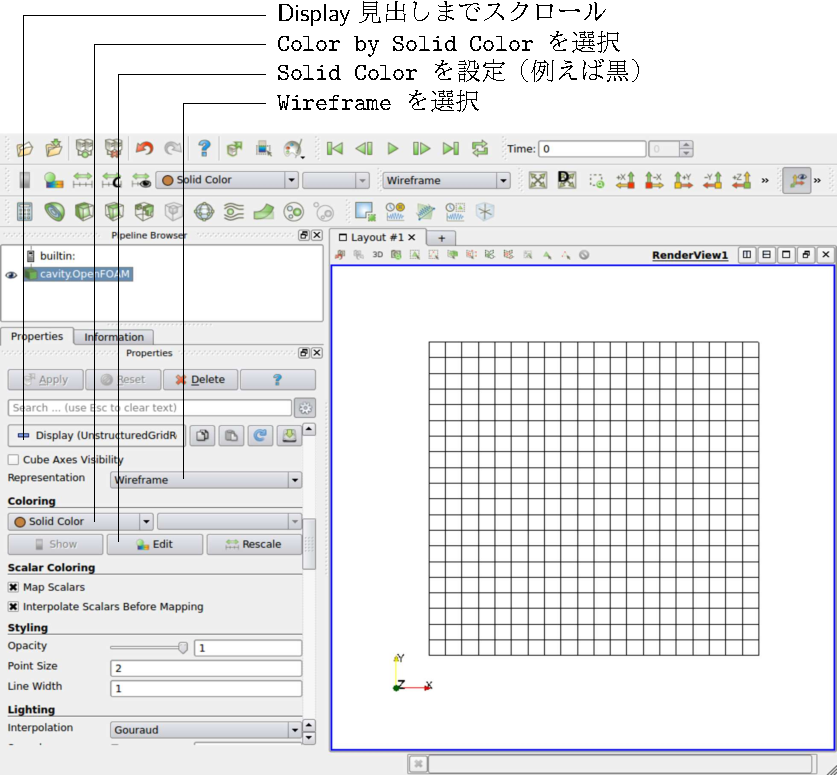
\includegraphics{fig-2-3}
\OFrevision{変更あり}%
 \caption{paraFoamでのメッシュの表示}
 \label{fig:2.3}
\end{figure}


\OFthirdparty{ParaView}を使うのがはじめてならば,
\autoref{ssec:6.1.5}で述べるように視点操作を試してみることをお勧めします.
特に本ケースは2次元なので,
\index{View Render@\PVpanel{View Render}!ウィンドウパネル}%
\index{ウィンドウパネル!View Render@\PVpanel{View Render}}%
\PVpanel{View Render}パネルの一番下付近にある
\index{Use Parallel Projection@\PVbutton{Use Parallel Projection}!ボタン}%
\index{ボタン!Use Parallel Projection@\PVbutton{Use Parallel Projection}}%
\PVbutton{Use Parallel Projection}を
選択するのがよいでしょう.
これは
\index{Propeties@\PVwindow{Propeties}!ウィンドウ}%
\index{ウィンドウ!Properties@\PVwindow{Properties}}%
\PVwindow{Properties}ウィンドウ最上部の検索窓の隣にある歯車のような
\index{Advanced Properties@\PVbutton{Advanced Properties}!ボタン}%
\index{ボタン!Advanced Properties@\PVbutton{Advanced Properties}}%
\PVbutton{Advanced Properties}ボタンが押されているときだけ現れます.
軸の方向は,
\index{Annotation@\PVpanel{Annotation}!ウィンドウパネル}%
\index{ウィンドウパネル!Annotation@\PVpanel{Annotation}}%
\PVpanel{Annotation}ウィンドウの
\index{Orientation Axes@\PVbutton{Orientation Axes}!ボタン}%
\index{ボタン!Orientation Axes@\PVbutton{Orientation Axes}}%
\PVbutton{Orientation Axes}をオン・オフするか,
マウスのドラッグ\&ドロップによって操作することができます.


\subsection{アプリケーションの実行}
\label{ssec:2.1.3}
あらゆるUNIX/Linuxの実行ファイルと同様に,
OpenFOAMアプリケーションは二つの方法で実行することができます.
一つ目は
\index{フォアグラウンド!プロセス}%
\index{プロセス!フォアグラウンド}%
フォアグラウンドのプロセスで,
コマンドプロンプトを与えるのにシェルが命令終了まで待つものです.
二つ目は
\index{バックグラウンド!プロセス}%
\index{プロセス!バックグラウンド}%
バックグラウンドプロセスで,
シェルがさらなる命令を受け入れるのに命令完了の必要がないものです.

ここでは,フォアグランドで
\index{icoFoam@\OFtool{icoFoam}!ソルバ}%
\index{ソルバ!icoFoam@\OFtool{icoFoam}}%
\OFtool{icoFoam}を動かしましょう.
\OFtool{icoFoam}ソルバはケースディレクトリ内に入って,
コマンドプロンプト上で
\begin{OFverbatim}[terminal]
icoFoam
\end{OFverbatim}
と入力することで実行できますが,

あるいはオプションに\texttt{-case}をつけることで
他のディレクトリからでも起動することができます.
\begin{OFverbatim}[terminal]
icoFoam -case $FOAM_RUN/tutorials/incompressible/icoFoam/cavity
\end{OFverbatim}%$
ジョブの進行過程は,ターミナルウィンドウに表示されます.
現在の時刻,最大Courant数,全てのフィールドの初期値と最終的結果を表示します.


\subsection{後処理}
\label{ssec:2.1.4}
結果が時刻ディレクトリに書かれるとすぐに,
\OFtool{paraFoam}を使って見ることができます.
\OFtool{para\-Foam}ウィンドウに戻って,
\texttt{cavity.OpenFOAM}ケースモジュールの
\index{Properties@\PVpanel{Properties}!ウィンドウパネル}%
\index{ウィンドウパネル!Properties@\PVpanel{Properties}}%
\PVpanel{Properties}パネルを選択してください.
ケースモジュールのパネルが存在していないようならば,
\texttt{cavity.OpenFOAM}が青くハイライトされているか,
それと並んだ目のボタンは表示が有効であることを示しているか,
を確認してください.

見たいデータを表示する\OFtool{paraFoam}を準備するには,
最初に必須の実行時間として$0.5\unit{s}$分のデータを読込まなければなりません.
ケースが実行中で一方\OFthirdparty{ParaView}を開いている場合,
時間ディレクトリの出力データは\OFthirdparty{ParaView}に自動的にロードはされません.
データをロードするためには,\PVwindow{Properties}ウィンドウで
\index{Refresh Times@\PVbutton{Refresh Times}!ボタン}%
\index{ボタン!Refresh Times@\PVbutton{Refresh Times}}%
\PVbutton{Refresh Times}をクリックします.
これで各時刻のデータが\OFthirdparty{ParaView}にロードされます.

\subsubsection{等値面とコンタプロット}
\label{sssec:2.1.4.1}
圧力を見るには
\index{Display@\PVpanel{Display}!ウィンドウパネル}%
\index{ウィンドウパネル!Display@\PVpanel{Display}}%
\PVpanel{Display}パネルに移動し,
選択したモジュールの表示形式を調整します.
単純な圧力分布を見るには\autoref{fig:2.4}に示すように
\PVkeyword{Representation}メニューで\PVkeyword{Surface}を選択し,
\PVkeyword{Coloring}で \includegraphics{icon-point-p} を選択して
\index{Rescale to Data Range@\PVbutton{Rescale to Data Range}!ボタン}%
\index{ボタン!Rescale to Data Range@\PVbutton{Rescale to Data Range}}%
\PVbutton{Rescale to Data Range}ボタンをクリックします.
$t = 0.5\unit{s}$における解析結果を表示するには,
\index{VCR Controls@\PVkeyword{VCR Controls}!メニュー}%
\index{メニュー!VCR Controls@\PVkeyword{VCR Controls}}%
\PVkeyword{VCR Controls}または
\index{Current Time Controls@\PVkeyword{Current Time Controls}!メニュー}%
\index{メニュー!Current Time Controls@\PVkeyword{Current Time Controls}}%
\PVkeyword{Current Time Controls}で現在時刻を0.5にします.
これらは\autoref{fig:6.4}に示すように
\OFthirdparty{ParaView}ウィンドウのトップメニューの下のツールバーの中に配置されています.
圧力場の解析結果は\autoref{fig:2.5}のようにキャビティの左上が低く,
右上が高い圧力分布になるはずです.

点アイコン (\includegraphics{icon-point-p}) では,圧力分布はセル間で補完された連続な分布として表示されます.
かわりに\OFkeyword{Coloring}でセルアイコン (\includegraphics{icon-cell-p}) を選択した場合,
各々のセルが単一の圧力値をもつものとして扱われ,各セルがグラデーションなしの単色で表示されます.

\PVkeyword{Active Variable Controls}ツールバー,
もしくは\PVpanel{Display}パネルの\OFkeyword{Coloring}にある
\PVbutton{Toggle Color Legend Visibility}ボタンをクリックすることで,
カラーバーを表示させることができます.
\PVkeyword{Active Variable Controls}ツールバーか
\PVpanel{Display}パネルの\PVpanel{Color}パネルにある
\PVkeyword{Edit Color Map}ボタンをクリックすると
フォントの大きさや種類,スケールの番号付けの形式など,
カラーバーの設定を変更することができます.
カラーバーはドラッグアンドドロップによりimageウィンドウに置くことも可能です.

\OFthirdparty{ParaView}では,
よく使われる青・緑・赤という(虹色の)カラースケールではなく,
青から白そして赤へと変化するカラースケールがデフォルトになっています.
そこで,はじめて\OFthirdparty{ParaView}を使うユーザは,
このカラースケールを変えたいと思うかもしれません.
これは,\PVwindow{Color Scale Editor}で\PVbutton{Choose Preset}ボタン(ハートが付いたアイコン)を選び,
\PVentry{Blue to Red Rainbow}を選択することで変更できます.
\PVbutton{OK}ボタンで確定したあとに,\PVbutton{Make Default}を押せば
\OFthirdparty{ParaView}はいつもこのタイプのカラーバーを使うようになります.

イメージを回転をさせるとすべての表面に圧力分布で色づけされていることが
確認できます.正しいコンタ図を得るために断面を作成するか,
\autoref{sssec:6.1.6.1}に示すsliceフィルタを用いてジオメトリを
スライスします.\autoref{sssec:6.1.6.1}に示すsliceフィルタを用います.
断面の中心座標は$(0.05, 0.05, 0.005)$,
基準点は$(0, 0, 1)$とします (\PVbutton{Z Normal}ボタンをクリックします).
断面を作成後,\autoref{ssec:6.1.6}に示すcontourフィルタによってコンタを描画します.


\begin{figure}[ht]
 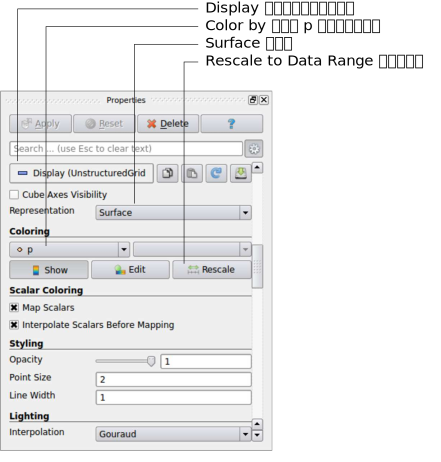
\includegraphics{fig-2-4}
\OFrevision{変更あり}%
 \caption{キャビティケースでの圧力等圧線の描画}
 \label{fig:2.4}
\end{figure}


\begin{figure}[ht]
 \includegraphics{fig-2-5}
 \caption{キャビティケースでの圧力}
 \label{fig:2.5}
\end{figure}


\subsubsection{ベクトルプロット}
\label{sssec:2.1.4.2}
流速ベクトルを描画する前に,先に作成した断面やコンタなどの
他のモジュールは不要なので取り除きましょう.
\PVwindow{Pipeline Browser}でそれらのモジュールを選択し,
Properties PanelのDeleteをクリックして削除するか,
\PVwindow{Pipeline Browser}で目の形のボタンをクリックして
それらのモジュールを非表示にします.

各格子の中心におけるベクトルグラフを作成することにしましょう.
まず,\autoref{sssec:6.1.7.1}に述べるように
格子の中心のデータのみに絞り込みます.
\PVwindow{Pipeline Browser}上で強調表示されている
cavity.OpenFOAMのモジュールを選択し,
Filter $\rightarrow$ AlphabeticalメニューからCell Centersを選択してApplyをクリックします.

\PVwindow{Pipeline Browser}で\PVkeyword{Centers}が強調表示された状態で,
Filter $\rightarrow$ CommonメニューからGlyphを選択します.
\autoref{fig:2.6}のような\PVpanel{Properties}ウィンドウが表示されます.
新たに選択したフィルタはFilter $\rightarrow$ Recentメニューに追加されることを覚えておきましょう
\footnote{訳注:原文ではFilter $\rightarrow$ Recentに\OFemph{移動}され,
元の場所には表示されなくなると書かれているが,そのような現象は確認できなかった.}%
.
この\PVpanel{Properties}パネルの\PVkeyword{vectors}メニューでは,
ベクトル場は速度のみなので,速度場\OFkeyword{U}が自動的に選択されています.
\PVkeyword{Scale Mode}は速度の\PVkeyword{Vector Magnitude}が初期値として選択されていますが,
領域全体を通る速度の様子を見るために,\PVkeyword{off}を選択し,
\PVentry{Set Scale Factor}を0.005にします.
\PVbutton{Apply}をクリックするとベクトルが表示されますが,単色,例えば白になっているでしょう.
通常は\PVpanel{Display}パネルで\PVkeyword{Color by U}を選択して速度に応じた色付けをします.
\PVkeyword{Edit Color Map}の中で\PVentry{Show Color Legend}を選択し,
速度の凡例を表示させましょう.出力結果は\autoref{fig:2.7}のようになります.
\index{Color Legend@\PVwindow{Color Legend}!ウィンドウ}%
\index{ウィンドウ!Color Legend@\PVwindow{Color Legend}}%
\PVwindow{Color Legend}(凡例)にはTimes Romanフォントが使用され,
\PVentry{Automatic Label Format}を解除して\PVentry{Label Format}テキストボックスに
\verb|%-#6.2f|を入力することで二つの有効数字でラベルを固定しています.
背景色は,\autoref{sssec:6.1.5.1}で述べるように,
\PVkeyword{View Settings}の\PVpanel{General}パネルで白に設定されています.

左右の壁において,ベトルが壁面を通り抜けるように見えていることに注意してください.
しかし,さらによく調べると,この壁に垂直な方向を向いている速度は$0$であることがわかります.
この少し混乱する状態は,スケーリングが\PVkeyword{off}で速度が$0$のとき,
\OFthirdparty{ParaView}は$x$方向のベクトルで表示するということに起因します.


\begin{figure}[ht]
 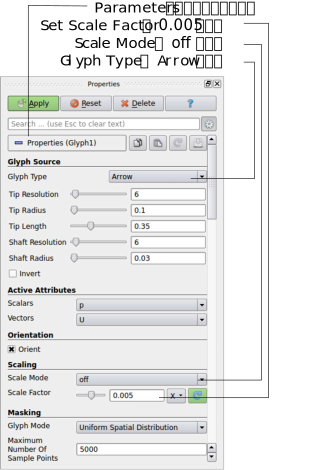
\includegraphics{fig-2-6}
\OFrevision{変更あり}%
 \caption{Glyphフィルタのパラメータパネル}
 \label{fig:2.6}
\end{figure}


\begin{figure}[ht]
 \includegraphics{fig-2-7}
 \caption{キャビティケースの速度}
 \label{fig:2.7}
\end{figure}


\subsubsection{流線プロット}
\label{sssec:2.1.4.3}
\OFthirdparty{ParaView}で後処理を続ける前に,
上述のベクトルプロットのモジュールは不要なので削除しましょう.
そうしたら,\autoref{ssec:6.1.8}の記述のように流速の流線をプロットしましょう.

\PVwindow{Pipeline Browser}で\texttt{cavity.OpenFOAM}モジュールをハイライトした状態で,
\PVmenu{Filter}メニューから\PVfilter{Stream Tracer}を選択し,\PVbutton{Apply}をクリックします.
そうすると,\autoref{fig:2.8}に示すように
\PVpanel{Propaties}ウィンドウが現れます.
\PVentry{Seed}の点は,ジオメトリの中心を垂直に通って,
\PVkeyword{High Resolutino Line Sourse}に沿うように (例えば$(0.05, 0, 0.005)$から
$(0.05, 0.1, 0.005)$まで) 指定しましょう.
このガイドに掲載した図では\PVentry{Point Resolution}を21に,
\PVentry{Maximum Step Length}を0.5に,
\PVentry{Initial Step Length}を0.2に,
\PVentry{Integration Direction}を\PVkeyword{BOTH}という設定を行いました.
また,\PVkeyword{Runge--Kutta 4/5} \PVentry{Integrator Type}は
デフォルトパラメータで使いました.

\PVbutton{Apply}をクリックすると,トレーサが生成されます.
そこで\PVmenu{Filter}メニューから\PVkeyword{Tubes}を選択することで,
高品質の流線図を作ることができます.
このレポートでは,次の設定を使いました.
\PVentry{Num.\ sides}を20,\PVentry{Radius}を0.003,\PVentry{Radius factor}を10にしました.
\PVbutton{Accept}を押すことで,\autoref{fig:2.9}ができます.


\begin{figure}[ht]
 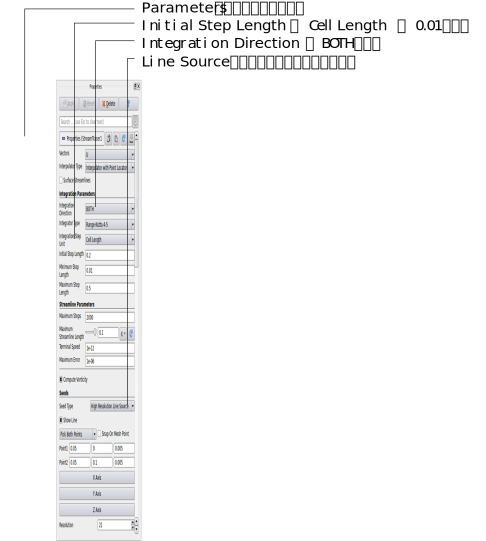
\includegraphics{fig-2-8}
\OFrevision{変更あり}%
 \caption{Stream Tracerフィルタのパラメータパネル}
 \label{fig:2.8}
\end{figure}


\begin{figure}[ht]
 \includegraphics{fig-2-9}
 \caption{キャビティケースの流線}
 \label{fig:2.9}
\end{figure}


\subsection{メッシュの解像度を増やす}
\label{ssec:2.1.5}
\index{メッシュ!かいぞうど@解像度}%
メッシュの解像度を各々の方向で2倍に増やします.
問題の初期条件として使うために,
粗いメッシュでの結果を,細かいメッシュ上に写像します.
そして,細かいメッシュの解を粗いメッシュの解と比較します.

\subsubsection{既存ケースを用いた新しいケースの作成}
\label{sssec:2.1.5.1}
\OFcase{cavity}をコピーし,
修正することで解析ケース\OFcase{cavityFine}を作成します.
まず\OFpath{cavity}と同じ階層に新しいディレクトリを作成します.
\begin{OFverbatim}[terminal]
cd $FOAM_RUN/tutorials/incompressible/icoFoam
mkdir cavityFine
\end{OFverbatim}%$
基本となる解析ケース\OFpath{cavity}の内容を
解析ケース\OFpath{cavityFine}にコピーし,
\OFpath{cavityFine}に移動します.
\begin{OFverbatim}[terminal]
cp -r cavity/constant cavityFine
cp -r cavity/system cavityFine
cd cavityFine
\end{OFverbatim}

\subsubsection{細かいメッシュの作成}
\label{sssec:2.1.5.2}
\OFtool{blockMesh}を使って計算格子数を増やしましょう.
\OFdictionary{blockMeshDict}ファイルをエディタで開き,
ブロックに関する記述を修正します.
ブロックを特定するには
\index{blocks@\OFkeyword{blocks}!キーワード}%
\index{キーワード!blocks@\OFkeyword{blocks}}%
\OFkeyword{blocks}というキーワードを用いましょう.
ブロック定義の対称性に関しては\autoref{sssec:5.3.1.3}で詳しく述べるので,
ここではhexが最初の頂点リストで,
各方向の計算格子の番号リストがあることを知ればよいでしょう.
これは,先の\OFcase{cavity}ケースでは\texttt{(20 20 1)}になっています.
これを\texttt{(40 40 1)}に変え,保存します.
ここで\OFtool{blockMesh}を実効することで新しい,
より細かいメッシュを生成することができます.

\subsubsection{粗いメッシュの結果を細かなメッシュにマッピングする}
\label{sssec:2.1.5.3}
\index{mapFields@\OFtool{mapFields}!ユーティリティ}%
\index{ユーティリティ!mapFields@\OFtool{mapFields}}%
\OFtool{mapFields}ユーティリティは,他のジオメトリの対応するフィールドの上へ
与えられたジオメトリに関した一つ以上のフィールドをマッピングします.
本チュートリアルの例では,入力フィールドと求める結果のフィールド両方の
ジオメトリ・境界の種類・境界条件が同一であるので,
フィールドは『首尾一貫している』と考えられます.
この例で\OFtool{mapFields}を実行するとき,
\texttt{-consistent}コマンドラインオプションを使います.

\OFtool{mapFields}がマッピングするフィールドデータは,
目的ケース(そのケースに結果がマッピングされる)の
\index{controlDict@\OFdictionary{controlDict}!ディクショナリ}%
\index{ディクショナリ!controlDict@\OFdictionary{controlDict}}%
\OFdictionary{controlDict}内の
\OFkeyword{startFrom}および\OFkeyword{startTime}で指定される時刻ディレクトリから読まれます.
この例では,\OFcase{cavityFine}ケースの細かいメッシュ上に\OFcase{cavity}ケースから
粗いメッシュの最終結果をマッピングしましょう.
これらの結果が\OFpath{cavity}の\OFpath{0.5}のディレクトリに格納されているので,
startTimeを\OFdictionary{controlDict}ディクショナリで$0.5\unit{s}$に,
startFromをstartTimeにセットします.これらの変更を保存しましょう.

\OFtool{mapFields}を実行する準備ができました.
\texttt{mapFields -help}と打ち込むと\OFtool{mapFields}の実行には入力ケースの
ディレクトリを指定する必要があることがわかります.
\texttt{-consistent}オプションを使うので,
次のようにユーティリティは\OFpath{cavityFine}ディレクトリから実行される.
\begin{OFverbatim}[terminal]
mapFields ../cavity -consistent
\end{OFverbatim}
\OFtool{mapFields}が実行され次のように出力されるでしょう.
\begin{OFverbatim}[baselinestretch=0.8, weight=\small]
Source: ".." "cavity"
Target: "." "cavityFine"

Create databases as time

Source time: 0.5
Target time: 0.5
Create meshes

Source mesh size: 400   Target mesh size: 1600

Consistently creating and mapping fields for time 0.5

    interpolating p
    interpolating U

End
\end{OFverbatim}

\subsubsection{設定の調整}
\label{sssec:2.1.5.4}
さて,全てのセルの寸法が半分になったので,
$1$より小さいCourant数を維持するためには\autoref{sssec:2.1.1.4}で述べるように
時間ステップを半分にしなければいけません.
deltaTを\OFdictionary{controlDict}ディクショナリにて$0.0025\unit{s}$に設定しましょう.
いままでは,フィールドデータを固定のステップ回数のもとでの時間間隔で
出力する方法を示してきましたが,
今回は固定の計算時間でデータ出力を指定する方法を示してみましょう.
\OFdictionary{controlDict}の\OFkeyword{writeControl}キーワード下において,
\index{timeStep@\OFkeyword{timeStep}!キーワードエントリ}%
\index{キーワードエントリ!timeStep@\OFkeyword{timeStep}}%
\OFkeyword{timeStep}エントリで固定のステップ回数で出力する代わりに,
\index{runTime@\OFkeyword{runTime}!キーワードエントリ}%
\index{キーワードエントリ!runTime@\OFkeyword{runTime}}%
\OFkeyword{runTime}を使って固定の計算時間を指定して結果を出力することができます.

このケースでは0.1ごとの出力を指定します.
したがって,\OFkeyword{writeControl}を\OFkeyword{runTime}に,
\index{writeInterval@\OFkeyword{writeInterval}!キーワード}%
\index{キーワード!writeInterval@\OFkeyword{writeInterval}}%
\OFkeyword{writeInterval}を0.1に設定しましょう.このようにすることで,
ケースは粗いメッシュでの解を入力条件として計算をはじめるので,
定常状態に収束するには適切な短い時間だけ動かせばよいのです.
したがって,\OFkeyword{endTime}は$0.7\unit{s}$でよいでしょう.
これらの設定が正しいことを確認し,ケースを保存しましょう.

\subsubsection{バックグラウンドプロセスとしてコードを動かす}
\label{sssec:2.1.5.5}
\OFtool{icoForm}をバックグラウンドプロセスとして動かしてみて,
最終的な結果を後で見ることができるように\OFpath{log}ファイルに出力しましょう.
\OFpath{cavitiyFine}ディレクトリにおいて次のコマンドを実行してください.
\begin{OFverbatim}[terminal]
icoFoam > log &
cat log
\end{OFverbatim}

\subsubsection{精密なメッシュによるベクトルプロット}
\label{sssec:2.1.5.6}
各々の新しいケースは本質的には単なるPipeline Browserに現れる
他のモジュールであるので,
\OFthirdparty{ParaView}で同時に複数のケースを開くことができます.
若干不便なことには,\OFthirdparty{ParaView}で新しいケースを開けるときには,
選ばれたデータが拡張子を含むファイル名である必要があります.
しかし,OpenFOAMにおいて,
各々のケースは特定のディレクトリ構造の中に拡張子なしで
複数のファイルに保存されます.
解決方法として,\OFtool{paraFoam}スクリプトが自動的に拡張子
\OFpath{.OpenFOAM}が付いたダミーファイルを作成することになっています.
それゆえに,\OFcase{cavity}ケースモジュールは
\texttt{cavity.OpenFOAM}と名づけられます.

\OFthirdparty{ParaView}内から他のケースディレクトリを開けたいならば,
そのようなダミーファイルを作成する必要があります.
たとえば,\OFcase{cavityFine}ケースを読み込むには,
コマンドプロンプトで次のようにタイプしてファイルを作成します.
\begin{OFverbatim}[terminal]
cd $FOAM_RUN/tutorials/incompressible/icoFoam
touch cavityFine/cavityFine.OpenFOAM
\end{OFverbatim}%$

こうしてFileメニューからOpen Dataを選んでディレクトリツリーをたどり,\break
\texttt{cavityFine.OpenFOAM}を選ぶことで,
cavityFineケースを\OFthirdparty{ParaView}に読み込めるようになりました.
さて,\OFthirdparty{ParaView}で精密なメッシュの結果の
ベクトルプロットを作ることができます.
同時に両方のケースのglyphを見られるようににすることによって,
\OFcase{cavityFine}ケースのプロットを\OFcase{cavity}ケースと比較することができます.


\begin{figure}[ht]
 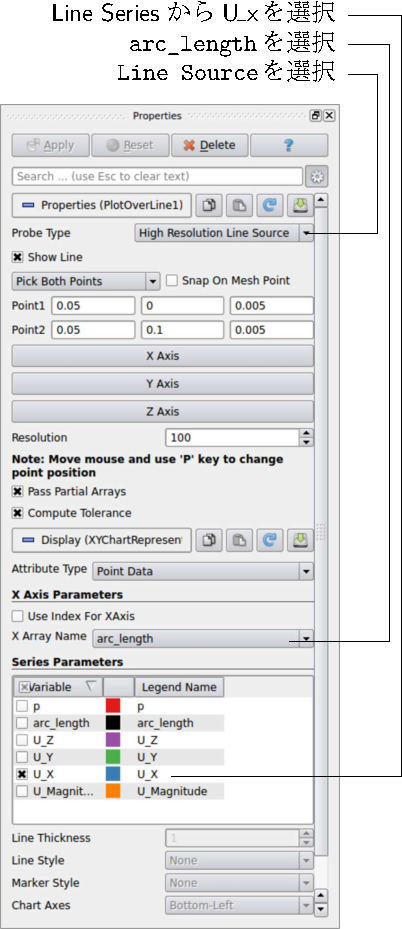
\includegraphics{fig-2-10}
\OFrevision{変更あり}%
 \caption{グラフ作図のためのフィールド選択}
 \label{fig:2.10}
\end{figure}


\subsubsection{グラフを描く}
\label{sssec:2.1.5.7}
OpenFOAMは,速度のスカラ値を抽出して2次元のグラフに
描画したい場合のデータの取り扱いに長けています.
データを操作するための特別なユーティリティが多数あり,
単純な計算を
\index{foamCalc@\OFtool{foamCalc}!ユーティリティ}%
\index{ユーティリティ!foamCalc@\OFtool{foamCalc}}%
\OFtool{foamCalc}によって組み合わせることができます.
次のようにユーティリティを指定して実行します.
\begin{OFverbatim}[terminal]
foamCalc <calcType> <fieldName1 ... fieldNameN>
\end{OFverbatim}
処理を規定する\texttt{<calcType>}には\texttt{addSubtract},
\texttt{randomise},\texttt{div},\texttt{components},\texttt{mag},
\texttt{magGrad},\texttt{magSqr},\texttt{interpolate}を指定することができます.
\texttt{<calcType>}のリストを見るには,
意図的に無効な処理を要求することでエラーメッセージとともに見ることができます.
\begin{OFverbatim}[baselinestretch=0.8, weight=\small]
>> foamCalc xxxx
Selecting calcType xxxx
unknown calcType type xxxx, constructor not in hash table
Valid calcType selections are:

8
(
randomise
magSqr
magGrad
addSubtract
div
mag
interpolate
components
)
\end{OFverbatim}

\OFkeyword{components}および\OFkeyword{mag}の\OFkeyword{calcType}はスカラ速度を計測するのに有用です.
ケースにて ``\texttt{foamCalc components U}'' を動かすと,
各時刻のディレクトリから速度のベクトル場を読み込み,
各ディレクトリに各軸方向成分のスカラ場
\OFkeyword{Ux},\OFkeyword{Uy},\OFkeyword{Uz}を書き出します.
同様に ``\texttt{foamCalc mag U}'' とは各時刻のディレクトリに
スカラ場\OFkeyword{magU}を書き込みます.

\OFtool{foamCalc}は\OFcase{cavity}と
\OFcase{cavityFine}のどちらに対しても実行することができます.
例えば\OFcase{cavity}に対しては,
以下のように\OFpath{cavity}ディレクトリに移動して\OFtool{foamCalc}を実行します.
\begin{OFverbatim}[terminal]
cd $FOAM_RUN/tutorials/incompressible/icoFoam/cavity
foamCalc components U
\end{OFverbatim}%$
それぞれの成分が\OFthirdparty{ParaView}内でグラフとして描画されます.
簡単に,早く,しかもラベル付けや形式化の調整ができるので,
とても高性能な出力を表示ができます.
しかしながら,出版用にグラフを作成するならばgnuplotやGrace/xmgrなどの
専用のグラフ描画ソフトを使って生データから作画するのがよいでしょう.
これを行うには,\autoref{sec:6.5}や\autoref{ssec:2.2.3}で述べる
\OFtool{sample}ユーティリティを使うとよいでしょう.

描画をする前に,新しく生成された\OFkeyword{Ux},\OFkeyword{Uy},\OFkeyword{Uz}のデータを
\OFthirdparty{ParaView}に読み込ませる必要があります.
これには,\texttt{cavity.OpenFOAM}モジュールのPropertiesパネルの上部にある
Refresh Timesをクリックします.
これにより,\OFthirdparty{ParaView}に新しいフィールドが読み込まれ,
Volume Fieldsウィンドウに現れます.
新しいフィールドを選択し,変更が適用されたことを確認します.
つまり,必要ならApplyを再度クリックします.
また,Mesh Partsパネルで境界領域が選択されているならば,
境界部分のデータ補間が不適切に行われています.
したがって,Mesh Partsパネルで,
\OFpatch{movingwall}や\OFpatch{fixedwall},\OFpatch{frontAndBack}といった
パッチの選択を解除して,変更を適用します.

さて,\OFthirdparty{ParaView}でグラフを表示してみましょう.
まずは描画したいモジュールを選択し,
\index{Plot Over Line@\PVfilter{Plot Over Line}!メニューエントリ}%
\index{メニューエントリ!Plot Over Line@\PVfilter{Plot Over Line}}%
\PVfilter{Plot Over Line}フィルタを\PVmenu{Filter} $\rightarrow$ \PVmenu{Data Analisys}から選択します.
\PVwindow{3D View}ウィンドウの下または横に新しい\PVwindow{XY Plot}ウィンドウが開きます.
\PVpanel{Properties}ウィンドウで線の終点を指定すると
Plobelineモジュールが作成されます.
この例ではPoint1を$(0.05, 0, 0.005)$,
Point2を$(0.05, 0.1, 0.005)$と指定して線を領域の中心の真上におきます.
Resolutionは100まで設定できます.

\PVbutton{Apply}をクリックすると\PVwindow{XY Plot}ウィンドウにグラフが描画されます.
\PVpanel{Display}パネルで,
\index{Attribute Mode@\PVmenu{Attribute Mode}!メニュー}%
\index{メニュー!Attribute Mode@\PVmenu{Attribute Mode}}%
\PVmenu{Attribute Mode}を\PVkeyword{Point Data}に設定します.
\PVkeyword{Use Data Array}オプションを\PVkeyword{X Axis Data}にし,
\verb|arc_length|オプションを加えて,
グラフの$x$軸データがキャビティの底からの距離になるようにできます.

\PVpanel{Display}ウィンドウの\PVpanel{Line Series}パネルから
表示するデータを選択することができます.
表示すべきスカラ場のリストからは,
ベクトルの大きさや成分が最初から利用可能であり,
例えば\OFkeyword{U\_X}と表示されています.
つまり,\OFkeyword{Ux}を\OFtool{foamCalc}から計算する必要はありません.
ここでは,\OFkeyword{Ux} (または\OFkeyword{U\_x}) 以外の系列の選択はすべて解除しましょう.
選択した系列の上の四角形の色が線の色です.
この上でダブルクリックをすれば簡単に変更することができます.

グラフの体裁を整えるには,\PVpanel{Line Series}パネルの下にある設定,
\PVkeyword{Line Color},\PVkeyword{Line Thickness},\PVkeyword{Line Style},
\PVkeyword{Marker Style},そして\PVkeyword{Chart Axes}を変更します.

また,\PVwindow{XY Plot}の左上にあるボタンをクリックすることもできます.
例えば,3番目のボタンでは,それぞれの軸のタイトルや凡例などを設定する
\PVentry{View Settings}を制御することができます.
また,軸のタイトルのフォント,色,配置,
値の範囲や線形・対数表示など,様々な設定を行うことができます.

\autoref{fig:2.11}は\OFthirdparty{ParaView}によって作画された図です.
望みどおりのグラフが作成できます.
\autoref{fig:2.11}は軸のオプションとして
Standard type of Notation,Specify Axis Rangeを選択し,
フォントはSans Serifの12ポイントです.
このグラフは点で表示していますが,
\PVpanel{Display}ウィンドウで
\index{Enable Line Series@\PVbutton{Enable Line Series}!ボタン}%
\index{ボタン!Enable Line Series@\PVbutton{Enable Line Series}}%
\PVbutton{Enable Line Series}ボタンを
有効にすれば線で表示できます.
注:もしこのボタンが,グレー表示で無効の状態になっていたら,
\PVpanel{Line Series}パネルでどれか変数を選択すれば有効になります.
\PVbutton{Enable Line Series}ボタンを選択しておけば,
\index{Line Style@\PVmenu{Line Style}!メニュー}%
\index{メニュー!Line Style@\PVmenu{Line Style}}%
\PVmenu{Line Style}や
\index{Marker Style@\PVmenu{Marker Style}!メニュー}%
\index{メニュー!Marker Style@\PVmenu{Marker Style}}%
\PVmenu{Marker Style}もユーザの好みで調整できます.


\begin{figure}[ht]
 \includegraphics{fig-2-11}
 \caption{\OFtool{paraFoam}でのグラフ作図}
 \label{fig:2.11}
\end{figure}


\subsection{勾配メッシュ}
\label{ssec:2.1.6}
解の誤差は,正しい解の形と選択した数値スキームで想定される形とが
大きく異なる領域で出ます.
例えば,数セルにわたる変数の線形変化に基づく数値スキームは,
正しい解自体が線形の場合にしか正確な解を導くことができません.
例えば勾配の変化が最も大きいところのような正しい解が
線形から一番大きく外れる領域で誤差は最も大きくなります.
セルの大きさに従って,誤差は減少します.

どんな問題も取りかかる前に解の概形の直感的予測ができるといいです.
次に,誤差が最も大きくなるところを予測し,メッシュ幅に勾配をつけ,
最も小さいセルがこれらの領域にくるようにします.
キャビティの場合,壁の近くで速度の大きい変化があることを予想できるので,
チュートリアルのこの部分では,メッシュがこの領域で,
より小さくなるように勾配付けします.
同じ数のセルを使用することによって,
コンピュータの負荷をあまり増加させずに,より精度を上げられます.

lid-drivenキャビティ問題のために壁に向かって勾配を付けた
$20 \times 20$セルのメッシュを作り,
\autoref{sssec:2.1.5.2}の細かいメッシュの結果を初期条件として
勾配付けされたメッシュに適用しましょう.
そして,勾配付けされたメッシュの結果を前のメッシュの結果と
比較してみましょう.
\index{blockMeshDict@\OFdictionary{blockMeshDict}!ディクショナリ}%
\index{ディクショナリ!blockMeshDict@\OFdictionary{blockMeshDict}}%
\OFdictionary{blockMeshDict}ディクショナリの書換えはとても重要であるので,
チュートリアルのこの部分を使ったケース (\OFpath{cavityGrade}) は
\OFpath{\$FOAM\_RUN/tutorials/incompressible/icoFoam}ディレクトリに入れておきました.

\subsubsection{勾配メッシュの作成}
\label{sssec:2.1.6.1}
ここで,四つの異なるメッシュ間隔の計算メッシュが計算領域の
上下左右のブロックに必要となります.
このメッシュのブロック構造を\autoref{fig:2.12}に示します.


\begin{figure}[ht]
 \includegraphics{fig-2-12}
 \caption{キャビティケースの勾配メッシュのブロック構造(ブロック番号)}
 \label{fig:2.12}
\end{figure}


\OFpath{cavityGrade}の\OFpath{system} (または\OFpath{constant/polyMesh}) サブディレクトリで
\OFdictionary{blockMeshDict}ファイルを見ることができます.
念のため\OFdictionary{blockMeshDict}の重要な要素を以下に述べます.
それぞれのブロックは$x$方向,$y$方向に10セルを有し,
もっとも大きなセルともっとも小さなセルとの大きさの比は2です.
\begin{OFverbatim}[file, linenum=17]
/*--------------------------------*- C++ -*----------------------------------*\
| =========                 |                                                 |
| \\      /  F ield         | OpenFOAM: The Open Source CFD Toolbox           |
|  \\    /   O peration     | Version:  2.3.0                                 |
|   \\  /    A nd           | Web:      www.OpenFOAM.com                      |
|    \\/     M anipulation  |                                                 |
\*---------------------------------------------------------------------------*/
FoamFile
{
    version     2.0;
    format      ascii;
    class       dictionary;
    object      blockMeshDict;
}
// * * * * * * * * * * * * * * * * * * * * * * * * * * * * * * * * * * * * * //

convertToMeters 0.1;

vertices        
(
    (0 0 0)
    (0.5 0 0)
    (1 0 0)
    (0 0.5 0)
    (0.5 0.5 0)
    (1 0.5 0)
    (0 1 0)
    (0.5 1 0)
    (1 1 0)
    (0 0 0.1)
    (0.5 0 0.1)
    (1 0 0.1)
    (0 0.5 0.1)
    (0.5 0.5 0.1)
    (1 0.5 0.1)
    (0 1 0.1)
    (0.5 1 0.1)
    (1 1 0.1)
);

blocks          
(
    hex (0 1 4 3 9 10 13 12) (10 10 1) simpleGrading (2 2 1)
    hex (1 2 5 4 10 11 14 13) (10 10 1) simpleGrading (0.5 2 1)
    hex (3 4 7 6 12 13 16 15) (10 10 1) simpleGrading (2 0.5 1)
    hex (4 5 8 7 13 14 17 16) (10 10 1) simpleGrading (0.5 0.5 1)
);

edges           
(
);

boundary
(
    movingWall
    {
        type wall;
        faces
        (
            (6 15 16 7)
            (7 16 17 8)
        );
    }
    fixedWalls
    {
        type wall;
        faces
        (
            (3 12 15 6)
            (0 9 12 3)
            (0 1 10 9)
            (1 2 11 10)
            (2 5 14 11)
            (5 8 17 14)
        );
    }
    frontAndBack
    {
        type empty;
        faces
        (
            (0 3 4 1)
            (1 4 5 2)
            (3 6 7 4)
            (4 7 8 5)
            (9 10 13 12)
            (10 11 14 13)
            (12 13 16 15)
            (13 14 17 16)
        );
    }
);

mergePatchPairs
(
);

// ************************************************************************* //
\end{OFverbatim}
いったんこのケースの\OFdictionary{blockMeshDict}ファイルを理解しておけば,
後はコマンドラインから\OFtool{blockMesh}を実行できます.
\autoref{ssec:2.1.2}に示した\OFtool{paraFoam}を使用することで
勾配付けされたメッシュを見ることができます.

\subsubsection{計算時間,時間ステップの変更}
\label{sssec:2.1.6.2}
最も速度が速くて最もサイズの小さいセルが上面に隣接するセルであり,
\autoref{sssec:2.1.1.4}で示したように,
この上面のセルにおいてCourant数が最大となります.
このようなことから上面に隣接するセルの大きさを見積もることは,
本ケースにて適当な時間ステップを計算する上で有効です.

一様でないメッシュ勾配を使用している場合,
\index{blockMesh@\OFtool{blockMesh}!ユーティリティ}%
\index{ユーティリティ!blockMesh@\OFtool{blockMesh}}%
\OFtool{blockMesh}は形状に関する数列をもちいてセルの大きさを算出します.
長さ$l$に沿って,最初と最後のセルとの間に,
比$R$の$n$個の計算セルが必要であるならば,
もっとも小さいセルの大きさは,次のように与えられます.
\begin{align}
 \label{eq:2.5}
  \Delta x_{\mathrm{s}} = l\frac{r - 1}{\alpha r - 1}
\end{align}
ここで,$r$はあるセルの大きさとその隣のセルの大きさとの比であり,
次式で表されます.
\begin{align}
 \label{eq:2.6}
  r = R^{\frac{1}{n-1}}
\end{align}
そして,
\begin{align}
 \label{eq:2.7}
  \alpha =
  \begin{cases}
   R & \text{for}\ R > 1, \\
   1 - r^{-1} + r^{-1} & \text{for}\ R < 1.
  \end{cases}
\end{align}
\OFcase{cavityGrade}ケースにおいては,各方向のセルの数は$10$であり,
最大セルと最小セルとの比は$2$,
ブロックの縦横は$0.05\unit{m}$です.
したがって,最小セルサイズは$3.45\unit{mm}$となります.
\autoref{eq:2.2} から時間ステップは,クラーン数を$1$以下に抑えるために
$3.45\unit{ms}$以下にしなければなりません.
有意な解析結果を得るためには,
時間ステップ\OFkeyword{deltaT}を$2.5\unit{ms}$まで小さくし,
\OFkeyword{writeInterval}を40とします.
これより解析結果は$0.1\unit{s}$ごとに書き出されることとなります.

このように,各設定に対応したファイルを編集することにより,
ケースディクショナリの各種条件を変更することができます.
ここで時間ないし計算経過の書き出しを操作したいならば,
\OFpath{/cavityGrade/system/controlDict}ファイル内に
それらのパラメータは納められており,
任意のエディタでこのファイルを開くことができます.
先に述べたように,計算を収束させるための保証として,
このケースでは時間ステップ\OFkeyword{deltaT}は\texttt{0.25e-3}に,
\OFkeyword{writeInterval}は40とします.

\OFkeyword{startTime}はその\OFcase{cavityFine}ケースの最終的な条件,
すなわち$0.7$に設定される必要があります.
\OFcase{cavity}と\OFcase{cavityFine}が規定された実行時間の中でよく収束させるためには,
\OFcase{cavityGrade}ケースのための実行時間を$0.1\unit{s}$に設定,
すなわち\OFkeyword{endTime}を0.8とします.

\subsubsection{解析場のマッピング}
\label{sssec:2.1.6.3}
\autoref{sssec:2.1.5.3}にあるように
\index{mapFields@\OFtool{mapFields}!ユーティリティ}%
\index{ユーティリティ!mapFields@\OFtool{mapFields}}%
\OFtool{mapFields}を使用して,
\OFcase{cavityFine}ケースの最終的な結果を
\OFcase{cavityGrade}ケースのメッシュにマッピングします.
以下のように\OFpath{cavityGrade}ディレクトリに入り,
\OFtool{mapFields}を実行してください.
\begin{OFverbatim}[terminal]
cd $FOAM_RUN/tutorials/incompressible/icoFoam/cavityGrade
mapFields ../cavityFine -consistent
\end{OFverbatim}%$
今度は,ケースディレクトリから\OFtool{icoFoam}を実行して,
計算実行時の情報をモニタリングします.
そして,\autoref{sssec:2.1.5.6}と\autoref{sssec:2.1.5.7}で説明した
後処理ツールを使って,収束した結果を見たり,他の結果と比較します.


\subsection{Reynolds数の増大}
\label{ssec:2.1.7}
これまで解いたケースはReynolds数が$10$でした.
これは大変に低い条件であり,
したがってキャビティの底部中央に小さな二次渦を伴うのみで,
迅速に安定解を導くことができました.
しかし,ここでReynolds数を$100$に上げると,
収束解を得るのにより長い時間を要することになります.
そこで\OFcase{cavity}ケースのメッシュを初期条件として使用することとします.
\OFpath{cavity}ケースディレクトリを\OFpath{cavityHighRe}という名前でコピーします.
\begin{OFverbatim}[terminal]
cd $FOAM_RUN/tutorials/incompressible/icoFoam
cp -r cavity cavityHighRe
\end{OFverbatim}%$

\subsubsection{後処理}
\label{sssec:2.1.7.1}
\OFpath{cavityHighRe}ケースに入り,
\index{transportProperties@\OFdictionary{transportProperties}!ディクショナリ}%
\index{ディクショナリ!transportProperties@\OFdictionary{transportProperties}}%
\OFdictionary{transportProperties}ディクショナリを編集します.
Reynolds数を10倍に増加させるためには,
動粘性係数を10分の1,すなわち$1 \times 10^{-3} \unit{m^{2}s^{-1}}$まで減らす必要があります.
これで\OFcase{cavity}ケースの実行結果から
\index{リスタート}%
リスタートして,このケースを実行できます.
これを実行するために,\OFkeyword{startFrom}キーワードを
\index{latestTime@\OFkeyword{latestTime}!キーワードエントリ}%
\index{キーワードエントリ!latestTime@\OFkeyword{latestTime}}%
\OFkeyword{latestTime}に
オプションを切り替えることにより,
\OFtool{icoFoam}は,最新の時間ディレクトリを初期データとして使用します(例えば0.5).
\OFkeyword{endTime}は$2\unit{s}$に設定し,本ケースを保存します.

\subsubsection{コードの実行}
\label{sssec:2.1.7.2}
まずはケースディレクトリから\OFtool{icoFoam}を実行し,ランタイム情報を見ます.
バックグラウンドでジョブを実行するときには,以下のUNIXコマンドが便利です.
\begin{description}
 \item[\texttt{nohup}]
            ユーザがログアウト後も稼働し続けるコマンド
 \item[\texttt{nice}]
            カーネル・スケジューラのジョブの優先順位を変えるコマンド.
            $-20$が最優先で,$19$は最も低い優先度.
\end{description}
これらのコマンドは,
例えば,ユーザがリモートマシンでケースを実行できるよう設定し,
頻繁にモニタしなくてもいいような場合,
リモートマシンではケース実行をあまり優先させたくないでしょうが,
そのような場合に便利です.
その場合,ユーザは\texttt{nohup}コマンドで稼働しているリモートマシンを
ログアウトしてジョブを実行し続けることができます.
一方,\texttt{nice}は優先度を19に設定します.
試しに,以下のようにコマンドを実行してみましょう.
\begin{OFverbatim}[terminal]
cd $FOAM_RUN/tutorials/incompressible/icoFoam
nohup nice -n 19 icoFoam > log &
cat log
\end{OFverbatim}%$
お気づきかもしれませんが,前述の解析方法では\OFtool{icoFoam}は,
速度\OFkeyword{U}の計算が止まっても,
それよりもずっと長い間もしくは解析が終わるまで
圧力\OFkeyword{p}の計算をし続けていました.
実際には,\OFtool{icoFoam}がいったん\OFkeyword{U}の計算をやめ,
\OFkeyword{p}の初期残差が\OFdictionary{fvSolution}ディクショナリで
設定された許容値(通常は$10^{-6}$)を下回ると
結果が効率的に収束するので,
フィールド・データをいったん時間ディレクトリに書き出して
計算を止めることができます.
例として,\OFcase{cavityHighRen}ケースの
\index{しゅうそく@収束}%
収束の\OFpath{log}ファイルを以下に示します.
示したとおり,$1.62\unit{s}$後に速度はすでに収束し,
初期の圧力残差は小さくなります.
\OFpath{log}において\verb|No Iterations 0|は,
\OFkeyword{U}の計算が止まったことを示しています.
\begin{OFverbatim}[file, linenum, weight=\scriptsize]
Time = 1.43

Courant Number mean: 0.221921 max: 0.839902
smoothSolver: Solving for Ux, Initial residual = 8.73381e-06, Final residual = 8.73381e-06, No Iterations 0
smoothSolver: Solving for Uy, Initial residual = 9.89679e-06, Final residual = 9.89679e-06, No Iterations 0
DICPCG: Solving for p, Initial residual = 3.67506e-06, Final residual = 8.62986e-07, No Iterations 4
time step continuity errors : sum local = 6.57947e-09, global = -6.6679e-19, cumulative = -6.2539e-18
DICPCG: Solving for p, Initial residual = 2.60898e-06, Final residual = 7.92532e-07, No Iterations 3
time step continuity errors : sum local = 6.26199e-09, global = -1.02984e-18, cumulative = -7.28374e-18
ExecutionTime = 0.37 s ClockTime = 0 s

Time = 1.435

Courant Number mean: 0.221923 max: 0.839903
smoothSolver: Solving for Ux, Initial residual = 8.53935e-06, Final residual = 8.53935e-06, No Iterations 0
smoothSolver: Solving for Uy, Initial residual = 9.71405e-06, Final residual = 9.71405e-06, No Iterations 0
DICPCG: Solving for p, Initial residual = 4.0223e-06, Final residual = 9.89693e-07, No Iterations 3
time step continuity errors : sum local = 8.15199e-09, global = 5.33614e-19, cumulative = -6.75012e-18
DICPCG: Solving for p, Initial residual = 2.38807e-06, Final residual = 8.44595e-07, No Iterations 3
time step continuity errors : sum local = 7.48751e-09, global = -4.42707e-19, cumulative = -7.19283e-18
ExecutionTime = 0.37 s ClockTime = 0 s
\end{OFverbatim}


\subsection{高Reynolds数流れ}
\label{ssec:2.1.8}
では,\OFtool{paraFoam}による結果を確認し,速度ベクトルを表示してください.
計算領域の角における二次渦が幾分増大していることがわかります.
このようなとき,ユーザは粘性係数を下げることにより
Reynolds数を増大させた計算ケースを再度実行できます.
渦の数が増加するにともない,より複雑な流れを解くために
当該領域でのメッシュ解像度を上げる必要がでてきます.
さらに,Reynolds数は収束に要する時間を増加させます.
このような場合,残差をモニタし,解を収束させるために
\OFkeyword{endTime}を延長したほうがよいでしょう.

空間および時間解像度の増加を要することは,
流れが乱流域に移行するという非現実的な状態となり,
解法の安定性の問題が生じることとなります.
もちろん,多くの工学的な問題は
極めて高いReynolds数条件となっており,
したがって,乱流挙動を直接解くのに多くのコストを負担することとなり,
実行不可能であります.
そのかわりに,
\index{らんりゅうモデル@乱流モデル!RAS}%
Reynolds平均シミューレション (RAS) 乱流モデルが
平均流れの挙動を解くのに用いられ,
乱れの統計値が計算されています.
壁関数を伴う標準$k$--$\varepsilon$モデルが
本チュートリアルの上面が移動する
キャビティケース(Reynolds数$10^{4}$)を解くのに用いられています.
二つの追加変数が解かれています.
それは,
\index{らんりゅう@乱流!うんどうエネルギ@運動エネルギ}%
乱流エネルギ$k$,
\index{らんりゅう@乱流!しょうさん@消散}%
乱流消散速度$\varepsilon$です.
乱流のための追加の方程式およびモデルは\OFtool{pisoFoam}と呼ばれる
OpenFOAMソルバにおいて実行されます.

\subsubsection{前処理}
\label{sssec:2.1.8.1}
\OFpath{\$FOAM\_RUN/tutorials/incompressible/pisoFoam/ras}ディレクトリの
\OFpath{cavity}ケースに移動します.
これまでと同様に,\OFtool{blockMesh}を走らせ,
メッシュを生成します.
壁関数付き標準$k$--$\varepsilon$モデルを用いる場合は,
壁近傍のセルにおける流れがモデル化されることにより,
壁方向へのメッシュ勾配は必ずしも必要ではありません.

OpenFOAMでは,様々な壁関数モデルを利用することができ,
それぞれのパッチの境界条件として設定します.
これにより,壁面ごとに異なる壁関数モデルを適用することが可能になります.
壁関数の選択は,乱流粘性係数$\nu_{\mathrm{t}}$の
ファイル\OFpath{0/nut}で指定します.
\begin{OFverbatim}[file, linenum=17]

dimensions      [0 2 -1 0 0 0 0];

internalField   uniform 0;

boundaryField
{
    movingWall
    {
        type            nutkWallFunction;
        value           uniform 0;
    }
    fixedWalls
    {
        type            nutkWallFunction;
        value           uniform 0;
    }
    frontAndBack
    {
        type            empty;
    }
}


// ************************************************************************* //
\end{OFverbatim}
このケースでは標準的な壁関数を採用し,
\OFpatch{movingWall}と\OFpatch{fixedWalls}のパッチに対して
\OFkeyword{nutWall\-Function}タイプを指定しています.
これ以外の壁関数モデルとしては,
粗壁面の壁関数\OFkeyword{nutRough\-WallFunction}などがあります.

次に,$k$と$\varepsilon$のファイル (\OFpath{0/k}と\OFpath{0/epsilon}) を開き,
境界条件を確かめます.
壁タイプの境界条件の選択には,
$\varepsilon$については\OFkeyword{epsilonWallFunction}境界条件を,
$k$については\OFkeyword{kqRWallFunction}を指定します.
後者は乱流運動エネルギの表現$k$,$q$,
あるいはReynolds応力$R$のいずれにも適用できる一般的な壁関数です.
$k$,$\varepsilon$の初期条件には,
速度変動$\bm{U}'$と
\index{らんりゅう@乱流!ながさスケール@長さスケール}%
乱流長さスケール$l$から推測した値を設定します.
$k$と$\varepsilon$は,これらのパラメタを用いて次式で表されます.
\begin{align}
 \label{eq:2.8}
  k &= \frac{1}{2}\overline{\bm{U}' \cdot \bm{U}'} \\
 \label{eq:2.9}
 \varepsilon &= \frac{C_{\mu}^{0.75}k^{1.5}}{l}
\end{align}
ここで$C_{\mu}$は$k$--$\varepsilon$モデルの定数であり,
その値は$0.09$です.Cartesian座標系では$k$は,
\begin{align}
 \label{eq:2.10}
 k = \frac{1}{2}({U_{x}'}^{2} + {U_{y}'}^{2} + {U_{z}'}^{2})
\end{align}
で表されます.各項は$x$,$y$,$z$方向速度乱れ成分です.
ここで,初期乱流が等方的であると仮定します.
例えば,${U_{x}'}^{2} = {U_{y}'}^{2} = {U_{z}'}^{2}$となり,
これら速度は上面速度の$5\unit{\%}$に等しく,
また,乱流長さスケール$l$はボックス幅$0.1\unit{m}$の
$5\unit{\%}$に等しいとすると,次のように表されます.
\begin{align}
 \label{eq:2.11}
 U_{x}' &= U_{y}' = U_{z}' = \frac{5}{100}1\unit{m\,s^{-1}} \\
 \label{eq:2.12}
 \Rightarrow k &= \frac{3}{2}\left(\frac{5}{100}\right)^{2}\unit{m^{2}s^{-2}}
 = 3.75 \times 10^{-3}\unit{m^{2}s^{-2}} \\
 \label{eq:2.13}
 \varepsilon &= \frac{C_{\mu}^{0.75}k^{1.5}}{l}
 \approx 7.54 \times 10^{-3}\unit{m^{2}s^{-3}}
\end{align}
上記のとおり$k$,$\varepsilon$を設定してください.
$U$と$p$に対する初期条件は前と同じように,
それぞれ$(0, 0, 0)$と$0$です.

OpenFOAMで提供されている乱流モデルには,
例えばRASやlarge-edy simulation (LES) のような,
さまざまな手法があります.
乱流のモデリング手法は
実行時に\OFdictionary{turbulenceProperties}ディクショナリの
\OFkeyword{simulationType}キーワードで選択できます.
このファイルは\OFpath{constant}ディレクトリの中に見つかります.
\begin{OFverbatim}[file, linenum=17]

simulationType  RAS;

RAS
{
    RASModel        kOmega;

    turbulence      on;

    printCoeffs     on;
}

// ************************************************************************* //
\end{OFverbatim}
\OFkeyword{simulationType}の選択肢は
\index{laminar@\OFkeyword{laminar}!キーワードエントリ}%
\index{キーワードエントリ!laminar@\OFkeyword{laminar}}%
\OFkeyword{laminar},
\index{RAS@\OFkeyword{RAS}!キーワードエントリ}%
\index{キーワードエントリ!RAS@\OFkeyword{RAS}}%
\OFkeyword{RAS},そして
\index{LES@\OFkeyword{LES}!キーワードエントリ}%
\index{キーワードエントリ!LES@\OFkeyword{LES}}%
\OFkeyword{LES}です (OpenFOAMバージョン3.0.0以前では
\index{RASModel@\OFkeyword{RASModel}!キーワードエントリ}%
\index{キーワードエントリ!RASModel@\OFkeyword{RASModel}}%
\OFkeyword{RASModel}と
\index{LESModel@\OFkeyword{LESModel}!キーワードエントリ}%
\index{キーワードエントリ!LESModel@\OFkeyword{LESModel}}%
\OFkeyword{LESModel}).
このケースで選択されている\OFkeyword{RAS}の場合,
RASモデリングの選択は
\index{RAS@\OFsubdictionary{RAS}!ディクショナリ}%
\index{ディクショナリ!RAS@\OFsubdictionary{RAS}}%
\OFsubdictionary{RAS}サブディクショナリ
(もしくは,OpenFOAMバージョン3.0.0以前では
\index{RASProperties@\OFdictionary{RASProperties}!ディクショナリ}%
\index{ディクショナリ!RASProperties@\OFdictionary{RASProperties}}%
\OFpath{RASProperties}という別ファイル) に記述します.
乱流モデルは\autoref{tbl:3.9}に示されている多くの使用可能なモデルから,
\OFkeyword{RASModel}エントリで選択します.
ここでは,標準$k$--$\varepsilon$モデルである\OFkeyword{kEpsilon}を選択します.
\OFkeyword{turbulence}のスイッチが\OFkeyword{on}になっていることも確認します.
乱流モデルに必要な係数には,それぞれのコードの中でデフォルト値が与えられています.
\index{printCoeffs@\OFkeyword{printCoeffs}!キーワード}%
\index{キーワード!printCoeffs@\OFkeyword{printCoeffs}}%
\OFkeyword{printCoeffs}というオプションのスイッチを\OFkeyword{on}にすると,
実行時に乱流モデルが呼ばれたときに,これらのデフォルト値が標準出力,
すなわちターミナルに出力されるようになります.
これらの係数は,モデル名に\OFkeyword{Coeffs}をつけた名前
(たとえば\OFkeyword{kEpsilon}モデルなら\OFkeyword{kEpsilonCoeffs})
のサブディクショナリとして表示されます.
モデルの係数は,必要に応じて\OFsubdictionary{RAS}サブディクショナリに
サブディクショナリを追加(コピー\&ペースト)し,値を適宜調整することで変更することができます.

次いで,
\index{transportProperties@\OFdictionary{transportProperties}!ディクショナリ}%
\index{ディクショナリ!transportProperties@\OFdictionary{transportProperties}}%
\OFdictionary{transportProperties}ディクショナリの層流
\index{ねんせいけいすう@粘性係数!どう@動\jdash}%
動粘性係数を設定します.
Reynolds数$10^{4}$を実現するために,
\autoref{eq:2.1} のReynolds数の定義式に示されるように,
動粘性係数を$10^{-5}\unit{m^{2}s^{-1}}$にする必要があります.

最後に,
\index{controlDict@\OFdictionary{controlDict}!ディクショナリ}%
\index{ディクショナリ!controlDict@\OFdictionary{controlDict}}%
\OFdictionary{controlDict}の\OFkeyword{startTime},
\OFkeyword{stopTime},\OFkeyword{deltaT},
そして\OFkeyword{writeInterval}を設定します.
Courant数の制限を満たすために\OFkeyword{deltaT}を$0.005\unit{s}$に設定し,
\OFkeyword{endTime}は$10\unit{s}$とします.

\subsubsection{コードの実行}
\label{sssec:2.1.8.2}
ケースディレクトリに入り,ターミナルで\texttt{pisoFoam}とタイプすることで
\OFtool{pisoFoam}を実行します.
粘性が小さいこの計算ケースでは,
移動している上面近傍の境界層は極めて薄く,
そして,上面に面するセルは比較的大きいことから,
上面速度よりもそれらセル中心の流体速度は極めて小さいです.
事実,100時間ステップ後,上面に隣接したセルにおける速度は,
上限である$0.2\unit{m\,s^{-1}}$程度です.
したがって最大Courant数は$0.2$以上にはなりません.
Courant数がより$1$に近接するように時間ステップを大きくし,
解析時間を増やすことは理にかなっています.
したがって,\OFkeyword{deltaT}を$0.02\unit{s}$にセットしなおし,
これに伴い,\OFkeyword{startFrom}を\OFkeyword{latestTime}にセットします.
本操作は,\OFtool{pisoFoam}が最新のディレクトリ,例えば\OFpath{10.0},
からスタートデータを読み込むように指示するものです.
\OFkeyword{endTime}は層流条件よりも収束に時間を要するため,
$20\unit{s}$にセットします.
従来どおり計算をリスタートし,解析の収束をモニタします.
解析が進行したら,連続した時間における結果を見てください.
そして解析が安定状態に収束するか,
もしくは周期的に振動しているか確認してください.
後者の場合には,収束は決して起こりませんが,
結果が不正確であるという意味ではありません.


\subsection{ケース形状の変更}
\label{ssec:2.1.9}
計算ケースの形状を変更し,新たな解析を行いたい場合,
新たな解析のスタート条件としてオリジナルの解析の全てないし一部を
保持しておくことは有効でしょう.
しかし,これは少し複雑になります.
なぜなら,オリジナルの解析の物理量が,
新しい解析ケースの物理量と一致しないからです.
しかし,
\index{mapFields@\OFtool{mapFields}!ユーティリティ}%
\index{ユーティリティ!mapFields@\OFtool{mapFields}}%
\OFtool{mapFields}ユーティリティは,形状や境界のタイプもしくは
その両者が不一致な場を位置づけることができます.

例であるように,\OFpath{icoFoam}ディレクトリ内にある
\OFpath{cavityClipped}ケースを開きます.
このケースは,標準的な\OFcase{cavity}ケースからなりますが,
底部右側,長さ$0.04\unit{m}$の正方形を除いたものであり,
\OFdictionary{blockMeshDict}は以下のようになっています.
\begin{OFverbatim}[file, linenum=17]
convertToMeters 0.1;

vertices
(
    (0 0 0)
    (0.6 0 0)
    (0 0.4 0)
    (0.6 0.4 0)
    (1 0.4 0)
    (0 1 0)
    (0.6 1 0)
    (1 1 0)

    (0 0 0.1)
    (0.6 0 0.1)
    (0 0.4 0.1)
    (0.6 0.4 0.1)
    (1 0.4 0.1)
    (0 1 0.1)
    (0.6 1 0.1)
    (1 1 0.1)

);

blocks
(
    hex (0 1 3 2 8 9 11 10) (12 8 1) simpleGrading (1 1 1)
    hex (2 3 6 5 10 11 14 13) (12 12 1) simpleGrading (1 1 1)
    hex (3 4 7 6 11 12 15 14) (8 12 1) simpleGrading (1 1 1)
);

edges
(
);

boundary
(
    lid
    {
        type wall;
        faces
        (
            (5 13 14 6)
            (6 14 15 7)
        );
    }
    fixedWalls
    {
        type wall;
        faces
        (
            (0 8 10 2)
            (2 10 13 5)
            (7 15 12 4)
            (4 12 11 3)
            (3 11 9 1)
            (1 9 8 0)
        );
    }
    frontAndBack
    {
        type empty;
        faces
        (
            (0 2 3 1)
            (2 5 6 3)
            (3 6 7 4)
            (8 9 11 10)
            (10 11 14 13)
            (11 12 15 14)
        );
    }
);

mergePatchPairs
(
);

// ************************************************************************* //
\end{OFverbatim}
\OFtool{blockMesh}を実行してメッシュを生成します.
パッチは\OFcase{cavity}ケースと同様に設定されています.
物理量の適用の過程を明確にするために,
元となるケース\OFcase{cavity}で\OFpatch{movingWall}であった
上側の壁は\OFpatch{lid}という名前に変更されています.

パッチが一致しない場合,
すべての物理量のデータが元のケースからマップされるという保証はありません.
残っているデータは元のケースと同一であるべきです.
したがってマッピングする前に時間のディレクトリに物理量のデータが
存在している必要があります.
\OFdictionary{controlDict}の\OFkeyword{startTime}が$0.5\unit{s}$に設定されているので
\OFcase{cavityClipped}ケースにおけるマッピングは
時刻$0.5\unit{s}$に予定されています.
したがって初期状態の物理量のデータ,
たとえば時刻0からをコピーする必要があります.
\begin{OFverbatim}[terminal]
cd $FOAM_RUN/tutorials/incompressible/icoFoam/cavityClipped
cp -r 0 0.5
\end{OFverbatim}%$

データをマッピングする前に$0.5\unit{s}$における形状と
物理量の状況をみておきましょう.

速度場と圧力場を\OFcase{cavity}から\OFcase{cavityClipped}にマップしようとしています.
パッチが一致しないため,
\OFpath{system}ディレクトリの\OFpath{mapFieldsDict}を編集する必要があります.
\OFkeyword{patchMap}と\OFkeyword{cutting\-Patches}という二つの入力項目があります.
\OFkeyword{patchMap}リストは元となる物理量のパッチとマッピング対象となる
物理量のパッチを含みます.対象物理量のパッチに
元となる物理量のパッチの値を引き継ぎたいときに利用します.
\OFcase{cavityClipped}において\OFpatch{lid}の境界値を
\OFcase{cavity}の\OFpatch{movingWall}から
引き継ぎたいので次のように\OFpath{patchMap}に記述します.
\begin{OFverbatim}[file]
patchMap
(
   lid movingWall
);
\end{OFverbatim}


\begin{figure}[ht]
 \includegraphics{fig-2-13}
 \caption{\OFcase{cavity}ケースで解いた速度場を
 \OFcase{cavityClipped}上にマッピングした図}
 \label{fig:2.13}
\end{figure}


\begin{figure}[ht]
 \includegraphics{fig-2-14}
 \caption{速度場の\OFcase{cavityClipped}の解法}
 \label{fig:2.14}
\end{figure}


\OFkeyword{cuttingPatches}リストは,対象パッチを削除した,
元の場の内部の値を写像した対象のパッチを含みます.
本ケースでは,\OFpatch{fixedWalls}を内挿プロセスの実例説明に用いることとします.
\begin{OFverbatim}[file]
cuttingPatches
(
  fixedWalls
);
\end{OFverbatim}
ここで,\OFtool{mapFields}を次のコマンドから実行することができます.
\begin{OFverbatim}[terminal]
mapFields ../cavity
\end{OFverbatim}
\autoref{fig:2.13}に示すような場を確認することができます.
境界パッチは,期待したように元のケースからの値が引き継がれています.
この実例において,\OFpatch{fixedWalls}パッチの速度を$(0, 0, 0)$に
リセットしたい場合があります.このときは,\OFpath{U}をエディタで開き,
\OFpatch{fixedWalls}を\OFkeyword{nonuniform}から
\OFkeyword{uniform (0,0,0)}に変更します.
そして,\OFtool{icoFoam}を実行しましょう.


\subsection{修正した形状の後処理}
\label{ssec:2.1.10}
最初と最後の解析の比較のために,この解析ケースのベクトル図を,
最初の時刻は$0.5\unit{s}$,
次いで$0.6\unit{s}$のように作成することができます.
さらに,幾何形状のアウトラインも示しますが,
これは2次元のケースでは少し注意が必要です.
\PVmenu{Filter}メニューから\PVfilter{Extract Parts}を選択し,
\PVpanel{Parameter}パネルで,興味のあるパッチ,
つまり\OFpatch{lid}と\OFpatch{fixedWalls}をハイライトします.
\PVbutton{Apply}ボタンをクリックし,\PVpanel{Display}パネルで
\PVkeyword{Wireframe}の選択すれば,
ジオメトリのうち選択したものを表示することができます.
\autoref{fig:2.14}は,パッチを黒で表示し,
修正した形状の底部角部分において形成される渦を示しています.



\section{穴あき板の応力解析}
\label{sec:2.2}
\index{あなあきいたのおうりょくかいせき@穴あき板の応力解析}%
\index{チュートリアル!あなあきいたのおうりょくかいせき@穴あき板の応力解析}%
本チュートリアルでは,中央に円形の穴を有する正方形板の
線形弾性定常応力解析における前処理,
実行および後処理の方法を述べます.
板の大きさは,辺長$4\unit{m}$および穴の半径$0.5\unit{m}$です.
さらに\autoref{fig:2.15}に示すように,
板の左右端には$\sigma = 10\unit{kPa}$の一様表面力が負荷されています.
本形状においては二つの対称面が存在するため,
解析領域は\autoref{fig:2.15}のグレーで示した板全体の
4分の1の部分のみをカバーすれば十分です.


\begin{figure}[ht]
 \includegraphics{fig-2-15}
 \caption{穴あき板の形状}
 \label{fig:2.15}
\end{figure}


本問題では,板の面内に応力が負荷されるため,
2次元問題として近似することができます.
Cartesian座標系においては,
この構造の3番目の次元についての振る舞いを考察するにあたって,
以下の二つの仮定をすることができます.
(1) 平面応力条件:2次元平面内以外の方向にはたらく応力成分を無視できるものと仮定します.
(2) 平面ひずみ条件:2次元平面内以外の方向にはたらくひずみ成分を無視できるものと仮定します.
本ケースのように3次元方向に薄い固体に対しては,
平面応力条件が適当です.
なお平面ひずみ条件は,3次元方向に厚い固体に対して適用されます.

円形の穴を有する無限大に大きく薄い板への負荷に対しては,
解析解が存在します.垂直な対称面における法線方向応力の解は以下となります.
\begin{align}
 \label{eq:2.14}
 (\sigma_{xx})_{x=0} =
 \begin{cases}
  \displaystyle
  \sigma\left(1 + \frac{R^{2}}{2y^{2}} + \frac{3R^{4}}{2y^{4}}\right)
  & \text{for}\ |y| \ge R \\
  0 & \text{for}\ |y| < R
 \end{cases}
\end{align}
シミュレーションの実行結果をこの解析解と比較することとしましょう.
チュートリアルの最後に,
メッシュの解像度および非等間隔化に対する解の感度を調べ,
また,穴に対する板の大きさを大きくすることで
無限大板に対する解析解と有限板に対する本問題の解を比較して
誤差を見積もることができるように演習問題を用意しています.


\subsection{メッシュ生成}
\label{ssec:2.2.1}
解析領域は4ブロックからなり,
そのうちのいくつかは円弧形の端部を有します.
$x$--$y$平面におけるメッシュブロックの構造を
\autoref{fig:2.16}に示します.
\autoref{sssec:2.1.1.1}で述べたように,
2次元として扱われるようなケースであっても,
OpenFOAMでは全てのジオメトリが3次元で生成されます.
したがって$z$方向のブロックの大きさを設定しなければなりませんので,
ここでは$0.5\unit{m}$とします.
表面力境界条件は力でなく応力で指定されますので,
断面積すなわち$z$方向の大きさは解に影響を与えません.


\begin{figure}[ht]
 \includegraphics{fig-2-16}
 \caption{穴あき板解析のためのメッシュのブロック構造}
 \label{fig:2.16}
\end{figure}


\OFpath{\$FOAM\_RUN/tutorials/stressAnalysis/solidDisplacementFoam}ディレクトリの
\OFpath{plateHole}ケースに移動し,\OFpath{plateHole}ケースの
\OFpath{blockMeshDict}をエディタで開きます.
\OFdictionary{block\-MeshDict}ディクショナリのエントリを以下に示します.
\begin{OFverbatim}[file, linenum=17]
convertToMeters 1;

vertices
(
    (0.5 0 0)
    (1 0 0)
    (2 0 0)
    (2 0.707107 0)
    (0.707107 0.707107 0)
    (0.353553 0.353553 0)
    (2 2 0)
    (0.707107 2 0)
    (0 2 0)
    (0 1 0)
    (0 0.5 0)
    (0.5 0 0.5)
    (1 0 0.5)
    (2 0 0.5)
    (2 0.707107 0.5)
    (0.707107 0.707107 0.5)
    (0.353553 0.353553 0.5)
    (2 2 0.5)
    (0.707107 2 0.5)
    (0 2 0.5)
    (0 1 0.5)
    (0 0.5 0.5)
);

blocks
(
    hex (5 4 9 10 16 15 20 21) (10 10 1) simpleGrading (1 1 1)
    hex (0 1 4 5 11 12 15 16) (10 10 1) simpleGrading (1 1 1)
    hex (1 2 3 4 12 13 14 15) (20 10 1) simpleGrading (1 1 1)
    hex (4 3 6 7 15 14 17 18) (20 20 1) simpleGrading (1 1 1)
    hex (9 4 7 8 20 15 18 19) (10 20 1) simpleGrading (1 1 1)
);

edges
(
    arc 0 5 (0.469846 0.17101 0)
    arc 5 10 (0.17101 0.469846 0)
    arc 1 4 (0.939693 0.34202 0)
    arc 4 9 (0.34202 0.939693 0)
    arc 11 16 (0.469846 0.17101 0.5)
    arc 16 21 (0.17101 0.469846 0.5)
    arc 12 15 (0.939693 0.34202 0.5)
    arc 15 20 (0.34202 0.939693 0.5)
);

boundary
(
    left
    {
        type symmetryPlane;
        faces
        (
            (8 9 20 19)
            (9 10 21 20)
        );
    }
    right
    {
        type patch;
        faces
        (
            (2 3 14 13)
            (3 6 17 14)
        );
    }
    down
    {
        type symmetryPlane;
        faces
        (
            (0 1 12 11)
            (1 2 13 12)
        );
    }
    up
    {
        type patch;
        faces
        (
            (7 8 19 18)
            (6 7 18 17)
        );
    }
    hole
    {
        type patch;
        faces
        (
            (10 5 16 21)
            (5 0 11 16)
        );
    }
    frontAndBack
    {
        type empty;
        faces
        (
            (10 9 4 5)
            (5 4 1 0)
            (1 4 3 2)
            (4 7 6 3)
            (4 9 8 7)
            (21 16 15 20)
            (16 11 12 15)
            (12 13 14 15)
            (15 14 17 18)
            (15 18 19 20)
        );
    }
);

mergePatchPairs
(
);

// ************************************************************************* //
\end{OFverbatim}
ここまで前のチュートリアルのように
直線的なエッジの形状を対象としてきましたが,
本チュートリアルでは曲線のエッジについて定義する必要があります.
\OFkeyword{edges}のキーワードエントリ(曲線エッジのリスト)内で
曲線エッジが定義されています.
それらのリストの構文では,最初に\OFkeyword{arc},
\OFkeyword{simpleSpline},\OFkeyword{polyLine}などの
曲線タイプが示されていますが,
さらに詳しくは\autoref{ssec:5.3.1}を参照してください.
この例題ではすべてのエッジが円弧なので\OFkeyword{arc}を使用します.
曲線を\OFkeyword{arc}で定義する際は始点と終点および
円弧上の点の3点によって指定します.

この
\index{blockMeshDict@\OFdictionary{blockMeshDict}!ディクショナリ}%
\index{ディクショナリ!blockMeshDict@\OFdictionary{blockMeshDict}}%
\OFdictionary{blockMeshDict}に含まれるブロック全てが
同じ方向を向いているわけではありません.
\autoref{fig:2.16}に示すように,
ブロック0の$x_{2}$方向はブロック4の$-x_{1}$方向と同じになっています.
このためブロック界面でセルが矛盾なく合うよう,
それぞれのブロックにおけるセルの番号および順序を
決定する際には注意を払わねばなりません.

プレートの全側面,穴の面,前後面の六つのパッチが定義されます.
そのうち左の面 (\OFpatch{left}) と下の面 (\OFpatch{down}) は対称面です.
このようなことはジオメトリ上の制限であるため,
ただの場の境界条件とするよりはメッシュの定義の中に組み込んで作ります.
よって,このパッチは\OFdictionary{blockMeshDict}内の
特別な\OFkeyword{SymmetryPlane}タイプを
使って定義するとよいでしょう.
\OFpatch{frontAndBack}パッチは2次元問題の場合は
無視される面を示しています.
これは先ほども言ったようにジオメトリ上の制限なので,
\OFdictionary{blockMeshDict}内の\OFkeyword{empty}タイプを使って定義しましょう.
境界条件に関してさらに詳しくは\autoref{ssec:5.2.1}を参照してください.
そのほかのパッチは通常の\OFkeyword{patch}タイプです.
メッシュは\OFtool{blockMesh}を使って生成し,
\autoref{ssec:2.1.2}に述べたようにして\OFtool{paraFoam}で見ることができます.
メッシュは\autoref{fig:2.17}のようになります.


\begin{figure}[ht]
 \includegraphics{fig-2-17}
 \caption{穴あき板問題のための解析メッシュ}
 \label{fig:2.17}
\end{figure}


\subsubsection{境界および初期条件}
\label{sssec:2.2.1.1}
メッシュの生成ができたら初期条件と境界条件を設定します.
熱抵抗を考慮しない応力解析では,
変位\OFkeyword{D}のみ設定する必要があります.
\OFpath{0/D}のファイルは以下のようになります.
\begin{OFverbatim}[file, linenum=17]
dimensions      [0 1 0 0 0 0 0];

internalField   uniform (0 0 0);

boundaryField
{
    left
    {
        type            symmetryPlane;
    }
    right
    {
        type            tractionDisplacement;
        traction        uniform (10000 0 0);
        pressure        uniform 0;
        value           uniform (0 0 0);
    }
    down
    {
        type            symmetryPlane;
    }
    up
    {
        type            tractionDisplacement;
        traction        uniform (0 0 0);
        pressure        uniform 0;
        value           uniform (0 0 0);
    }
    hole
    {
        type            tractionDisplacement;
        traction        uniform (0 0 0);
        pressure        uniform 0;
        value           uniform (0 0 0);
    }
    frontAndBack
    {
        type            empty;
    }
}

// ************************************************************************* //
\end{OFverbatim}
まず,変位の初期条件が$(0, 0, 0)\unit{m}$になっています.
\OFpath{Constant/polyMesh/boundaries}のメッシュの記述にあるように,
\OFpatch{left}と\OFpatch{down}のパッチは
\OFkeyword{type}が\OFkeyword{symmetryPlane}である必要があります.
同様に\OFpatch{frontAndBack}は\OFkeyword{empty}になります.

その他のパッチは表面力境界条件です.表面力境界条件は,
(1) キーワード
\index{traction@\OFkeyword{traction}!キーワード}%
\index{キーワード!traction@\OFkeyword{traction}}%
\OFkeyword{traction}で表される,境界面における表面力ベクトル,
(2) キーワード
\index{pressure@\OFkeyword{pressure}!キーワード}%
\index{キーワード!pressure@\OFkeyword{pressure}}%
\OFkeyword{pressure}で表される,
境界面の法線方向に働く表面力となる(外向きの場合は負値となる)圧力,
の線形結合で指定されます.
\OFpatch{up}および\OFpatch{hole}パッチは表面力ゼロであるため,
表面力ベクトルおよび圧力ともにゼロが設定されます.
\OFpatch{right}パッチについては,\autoref{fig:2.24}に示すように,
表面力ベクトルは$(1\mathrm{e}4, 0, 0)\unit{Pa}$,
圧力は$0\unit{Pa}$が設定されます.
変位の初期条件は全て$(0, 0, 0)\unit{m}$が設定されます.

\subsubsection{機械的性質}
\label{sssec:2.2.1.2}
本ケースにおける物性値は
\index{mechanicalProperties@\OFdictionary{mechanicalProperties}!ディクショナリ}%
\index{ディクショナリ!mechanicalProperties@\OFdictionary{mechanicalProperties}}%
\OFdictionary{mechanicalProperties}ディクショナリによって設定します.
本問題においては,\autoref{tbl:2.1}に示す
鋼の機械的性質を指定する必要があります.
さらに本ディクショナリで\OFkeyword{planeStress}を\OFkeyword{yes}に設定しなければなりません.


\begin{table}[ht]
 %#! uplatex UserGuideJa
\begin{tabular}{lccc}
 物性 & 単位 & キーワード & 値 \\
 \hline
 \tblstrut
 密度 & $\unit*{kg\,m^{-3}}$ & \OFkeyword{rho} & 7854 \\
 Young率 & $\unit*{Pa}$ & \OFkeyword{E} & $2 \times 10^{11}$ \\
 Poisson比 & --- & \OFkeyword{nu} & 0.3 \\
 \hline
\end{tabular}

 \caption{鋼の機械的性質}
 \label{tbl:2.1}
\end{table}


\subsubsection{熱的性質}
\label{sssec:2.2.1.3}
運動によって発生する熱応力によって
運動方程式と連成した熱方程式を解くことができるよう,
\index{solidDisplacementFoam@\OFtool{solidDisplacementFoam}!ソルバ}%
\index{ソルバ!solidDisplacementFoam@\OFtool{solidDisplacementFoam}}%
\OFtool{solidDisplacementFoam}ソルバには温度場を表す変数\OFkeyword{T}が存在します.
\index{thermalProperties@\OFdictionary{thermalProperties}!ディクショナリ}%
\index{ディクショナリ!thermalProperties@\OFdictionary{thermalProperties}}%
\OFdictionary{thermalProperties}ディクショナリの\OFkeyword{thermalStress}スイッチによって,
OpenFOAMが熱方程式を解くべきかどうかを実行時に指定します.
また本ディクショナリによって,
本ケースすなわち\autoref{tbl:2.2}に示す
鋼の熱的性質を指定します.


\begin{table}[ht]
 %#! uplatex UserGuideJa
\begin{tabular}{lccc}
 物性 & 単位 & キーワード & 値 \\
 \hline
 \tblstrut
 比熱容量 & $\unit*{J\,kg^{-1}K^{-1}}$ & \OFkeyword{C} & 434 \\
 熱伝導率 & $\unit*{W\,m^{-1}K^{-1}}$ & \OFkeyword{k} & 60.5 \\
 熱膨張率 & $\unit*{K^{-1}}$ & \OFkeyword{alpha} & $1.1 \times 10^{-5}$ \\
 \hline
\end{tabular}

 \caption{鋼の熱的性質}
 \label{tbl:2.2}
\end{table}


本ケースにおいては熱の方程式は解きません.
したがって\OFdictionary{thermalProperties}ディクショナリにおける
\OFkeyword{thermalStress}キーワードエントリは\OFkeyword{no}に設定します.

\subsubsection{制御}
\label{sssec:2.2.1.4}
通常どおり,解法の制御に関する情報は\OFdictionary{controlDict}ディクショナリから
読み込まれます.本ケースでは,\OFkeyword{startTime}は0です.
本ケースは定常状態ですので,時間刻みは重要ではありません.
このような状況では,
定常状態のケースにおける反復回数カウンタとして働くよう,
時間刻み\OFkeyword{deltaT}を1に設定するのが最善です.
このようにした場合,本ケースで100に設定した\OFkeyword{endTime}は
反復回数の上限として働きます.\OFkeyword{writeInterval}は20に設定します.

\index{controlDict@\OFdictionary{controlDict}!ディクショナリ}%
\index{ディクショナリ!controlDict@\OFdictionary{controlDict}}%
\OFdictionary{controlDict}のエントリは以下のようになります.
\begin{OFverbatim}[file, linenum=17]

application     solidDisplacementFoam;

startFrom       startTime;

startTime       0;

stopAt          endTime;

endTime         100;

deltaT          1;

writeControl    timeStep;

writeInterval   20;

purgeWrite      0;

writeFormat     ascii;

writePrecision  6;

writeCompression off;

timeFormat      general;

timePrecision   6;

graphFormat     raw;

runTimeModifiable true;


// ************************************************************************* //
\end{OFverbatim}

\subsubsection{離散化スキームおよび線形方程式ソルバ制御}
\label{sssec:2.2.1.5}
次は\OFdictionary{fvSchemes}ディクショナリについて見てみましょう.
まず,この問題は定常状態ですので,
\OFkeyword{timeScheme}における時間微分としては\OFkeyword{steadyState}を選択します.
これによって時間微分項がオフの状態になります.
全てのソルバが定常状態および過渡的状態の双方に対して
適用可能な訳ではありませんが,
\OFtool{solidDisplacementFoam}は基本的なアルゴリズムが
双方のシミュレーションともに共通であるため,
双方に適用可能となっています.

線形弾性応力解析における運動方程式には,
変位の勾配を含む陽な項がいくつか存在します.
この勾配を正確かつ滑らかに評価できれば,良い計算結果が得られます.
通常,有限体積法における離散化は,
\index{こうばい@勾配!Gaussのていり@Gaussの定理}%
Gaussの定理に基づいています.
Gauss法は大抵の目的においては十分に正確ですが,
本ケースにおいては
\index{こうばい@勾配!さいしょうにじょうフィット@最小二乗フィット}%
\index{こうばい@勾配!さいしょうにじょうほう@最小二乗法}%
最小二乗法を使用することとします.
したがって
\index{fvSchemes@\OFdictionary{fvSchemes}!ディクショナリ}%
\index{ディクショナリ!fvSchemes@\OFdictionary{fvSchemes}}%
\OFdictionary{fvSchemes}ディクショナリを開き,
\OFkeyword{grad(U)}勾配離散化スキームとして
\index{leastSquares@\OFkeyword{leastSquares}!キーワード}%
\index{キーワード!leastSquares@\OFkeyword{leastSquares}}%
\OFkeyword{leastSquares}を選択してください.
\begin{OFverbatim}[file, linenum=17]

d2dt2Schemes
{
    default         steadyState;
}

ddtSchemes
{
    default         Euler;
}

gradSchemes
{
    default         leastSquares;
    grad(D)         leastSquares;
    grad(T)         leastSquares;
}

divSchemes
{
    default         none;
    div(sigmaD)     Gauss linear;
}

laplacianSchemes
{
    default         none;
    laplacian(DD,D) Gauss linear corrected;
    laplacian(DT,T) Gauss linear corrected;
}

interpolationSchemes
{
    default         linear;
}

snGradSchemes
{
    default         none;
}

// ************************************************************************* //
\end{OFverbatim}
\OFpath{system}ディレクトリにある
\OFdictionary{fvSolution}ディクショナリでは,
求解に使用される線形方程式のソルバおよびアルゴリズムを設定します.
まず\OFsubdictionary{solvers}サブディクショナリを見ると,
\OFkeyword{D}の
\index{solver@\OFkeyword{solver}!キーワード}%
\index{キーワード!solver@\OFkeyword{solver}}%
\OFkeyword{solver}が
\index{GAMG@\OFkeyword{GAMG}!キーワードエントリ}%
\index{キーワードエントリ!GAMG@\OFkeyword{GAMG}}%
\OFkeyword{GAMG}になっていることがわかります.
\index{tolerance@\OFkeyword{tolerance}!キーワード}%
\index{キーワード!tolerance@\OFkeyword{tolerance}}%
\OFkeyword{tolerance}で表される
ソルバ許容値(ソルバ名の次の数値)は,本問題では$10^{-6}$を設定します.
\index{relTol@\OFkeyword{relTol}!キーワード}%
\index{キーワード!relTol@\OFkeyword{relTol}}%
\OFkeyword{relTol}で表される
ソルバの相対許容値(さらにその次の数値)には
各反復ごとの残差の所要低減量を設定します.
本問題においては多くの項が陽であり,
また個別の反復的手順の一部としてアップデートされるため,
各反復において厳しい相対許容値を設定することは非効率的です.
したがって相対許容値として合理的な値は$0.01$,
もしくはさらに高めの$0.1$,
あるいはせいぜいこのケースのように$0.9$程度にしておきます.
\begin{OFverbatim}[file, linenum=17]

solvers
{
    "(D|T)"
    {
        solver          GAMG;
        tolerance       1e-06;
        relTol          0.9;
        smoother        GaussSeidel;
        cacheAgglomeration true;
        nCellsInCoarsestLevel 20;
        agglomerator    faceAreaPair;
        mergeLevels     1;
    }
}

stressAnalysis
{
    compactNormalStress yes;
    nCorrectors     1;
    D               1e-06;
}


// ************************************************************************* //
\end{OFverbatim}
\OFdictionary{fvSolution}ディクショナリは,
アプリケーションソルバに特有の制御パラメータを含む
\OFsubdictionary{stressAnalysis}サブディクショナリを含みます.
まず,各時刻ステップ内での表面力境界条件処理を含めた,
全方程式系に関する外側ループの数を指定する\OFkeyword{nCorrectors}があります.
本問題は定常状態を扱いますので,
「時刻ステップ」を反復回数カウンタとして使い収束解へと向かう
反復を実行することになります.
したがって\OFkeyword{nCorrectors}を1に設定します.

\OFkeyword{D}キーワードには外側反復ループにおける収束許容値,
すなわち初期残差に対して反復計算によって消去されるべき
レベルを設定します.
本問題では前述において設定したソルバ許容値の$10^{-6}$に設定します.


\subsection{コードの実行}
\label{ssec:2.2.2}
以下に示すようなコマンドによって,
実行後にログファイルに記録された収束状況を見ることができるよう,
バックグラウンドでコードを実行します.
\begin{OFverbatim}[terminal]
cd $FOAM_RUN/tutorials/stressAnalysis/solidDisplacementFoam/plateHole
solidDisplacementFoam > log &
\end{OFverbatim}%$
実行後には生成されたログファイルを見て,
反復回数および解を求める各方向変位の初期・最終残差などの
収束状況を確認できます.
本ケースの反復許容回数設定では,
最終残差は必ず初期残差の$0.1$倍以下となるはずです.
いったん両初期残差ともに$10^{-6}$の収束許容残差以下となれば,
その計算は収束したとみなしバッチジョブを\texttt{kill}することによって
止めることができます.


\subsection{後処理}
\label{ssec:2.2.3}
後処理は\autoref{ssec:2.1.4}と
同様に行うことができます.
\OFtool{solidDisplacementFoam}ソルバは,
応力場$\sigma$を対称テンソル場として出力します.
したがって例えば,$\sigma_{xx}$を\OFtool{paraFoam}で見ることができます.
OpenFOAMソルバにおける変数名は通常,
それらを表す数学記号にならって名付けられることは,
ここで再度述べるに値するでしょう.ギリシア記号の場合は,
変数は発音どおりに名付けられます.例えば,
$\sigma_{xx}$は\OFkeyword{sigmaxx}と名付けられます.

独立したスカラ成分の$\sigma_{xx}$や$\sigma_{xy}$などは,
\autoref{sssec:2.1.5.7}で述べた\OFtool{foamCalc}を\OFkeyword{sigma}に関して実行して求めます.
\begin{OFverbatim}[terminal]
foamCalc components sigma
\end{OFverbatim}
\OFkeyword{sigmaxx}や\OFkeyword{sigmaxy}などと名づけられた成分の
ファイルが時間のディレクトリに生成されます.
\autoref{fig:2.18}のように応力を\OFtool{paraFoam}で見ることができます.


\begin{figure}[ht]
 \includegraphics{fig-2-18}
 \caption{穴あき板における応力場}
 \label{fig:2.18}
\end{figure}


\autoref{eq:2.14} の解析解と
ここで得られた数値解を比較しましょう.
そのためには,解析領域左端の対称面に沿ってのデータを
出力しなければなりません.
このようなグラフのために必要なデータは,
\OFtool{sample}ユーティリティによって作成することができます.
\OFtool{sample}の設定は\OFpath{system}ディレクトリ内の\OFpath{sampleDict}で行い
詳細は\autoref{tbl:6.3}に要約しています.
データのサンプリングを行う座標区間は,
\OFkeyword{sets}によって$(0.0, 0.5, 0.25)$から$(0.0, 2.0, 0.25)$に指定されています.
物理量は\OFkeyword{fields}に指定します.
\begin{OFverbatim}[file, linenum=17]

interpolationScheme cellPoint;

setFormat       raw;

sets
(
    leftPatch
    {
        type    uniform;
        axis    y;
        start   (0 0.5 0.25);
        end     (0 2 0.25);
        nPoints 100;
    }
);

fields          (sigmaEq);


// ************************************************************************* //
\end{OFverbatim}
通常通り\OFtool{sample}を実行してください.
\index{writeFormat@\OFkeyword{writeFormat}!キーワード}%
\index{キーワード!writeFormat@\OFkeyword{writeFormat}}%
\OFkeyword{writeFormat}は\OFkeyword{raw}形式で2列のフォーマットとなっています.
データは\OFpath{postProcessing/sets}ディレクトリの時刻サブディレクトリの中のファイルに書き込まれます.
たとえば,時刻$t = 100\unit{s}$のデータは
\OFpath{postProcessing/sets/100/leftPatch\_sigmaxx.xy}に書き込まれます.
GnuPlotのようなアプリケーションでは,
コマンドプロンプトで以下を入力することで,
数値解および解析解の両方をプロットすることができます.
\begin{OFverbatim}[terminal]
plot [0.5:2] [0:] 'postProcessing/sets/100/leftPatch_sigmaxx.xy',
     1e4*(1+(0.125/(x**2))+(0.09375/(x**4)))
\end{OFverbatim}
プロット例を\autoref{fig:2.19}に示します.


\begin{figure}[ht]
 \includegraphics{fig-2-19}
 \caption{垂直方向対称面における法線方向応力}
 \label{fig:2.19}
\end{figure}


\subsection{演習}
\label{ssec:2.2.4}
以下は\OFtool{solidDisplacementFoam}に習熟していただくための演習課題です.

\subsubsection{メッシュ解像度の増加}
\label{sssec:2.2.4.1}
$x$,$y$方向それぞれのメッシュ解像度を増やしてみましょう.
\autoref{ssec:2.2.3}の最終的な粗メッシュの結果を,
\index{mapFields@\OFtool{mapFields}!ユーティリティ}%
\index{ユーティリティ!mapFields@\OFtool{mapFields}}%
\OFtool{mapFields}を使って密メッシュの初期条件にマッピングしてください.

\subsubsection{非等間隔メッシュの導入}
\label{sssec:2.2.4.2}
穴に近いセルが遠いセルより密になるよう,
メッシュ幅を変化させてください.
隣接するセルの大きさの比率が$1.1$以上にならないように,
またブロック間のセルの大きさの比率がブロック内の比率と
同様となるようメッシュを作成してください.
メッシュの非等間隔化については\autoref{ssec:2.1.6}で述べました.
ここでも,\autoref{ssec:2.2.3}の最終的な粗メッシュでの結果を,
\OFtool{mapFields}を使って非等間隔メッシュの初期条件としてマッピングします.
結果を解析解および非等間隔化する前の結果と比較してみましょう.
等間隔メッシュと同一のセル数を使用した場合,
解の精度は改善されるでしょうか?

\subsubsection{板の大きさの変更}
\label{sssec:2.2.4.3}
ここで示されている解析解は,
有限な大きさの穴を有する無限大板におけるものです.
したがって有限な大きさの板においては,
この解析解は必ずしも正確ではありません.
誤差を見積もるために,
穴の大きさを同一に保ったまま板を大きくしてみましょう.



\section{ダムの決壊}
\label{sec:2.3}
\index{ダムのけっかい@ダムの決壊}%
\index{チュートリアル!ダムのけっかい@ダムの決壊}%
このチュートリアルでは,\OFtool{interFoam}を用いて,
単純化したダム決壊の2次元問題を解くことにします.
この問題の特徴は,くっきりとした界面や
\index{じゆうひょうめん@自由表面}%
自由表面によって
隔てられている二つの流体による非定常の流れ場であることです.
\OFtool{interFoam}における2相流体を解くアルゴリズムは,
Volume of fluid (VOF) 法によるものであり,
ここでは特別な輸送方程式を解いて,
計算格子における2相の体積分率,
もしくは相比率$\alpha$を決定します.
各物理量は,この相比率に(各流体の)密度をかけた
平均的な値として算出されます.
個々の物質の界面は,VOF法ではその性質上明示的には解かれず,
相比率場の特性として浮き上がってくるということになります.
相比率は0から1の間の任意の値をとり得るため,
界面は決してくっきりと定義されませんので,
本来のくっきりとした界面が存在するべき領域の周辺を,
(計算上の)界面がぼんやりと占めることになります.

計算条件では,貯水池の左側に,膜で仕切られた水柱が最初存在します.
時刻$t = 0\unit{s}$に,膜が取り除かれて,水柱が崩れだします.
崩壊しながら,水流は貯水槽の底にある出っ張りにぶつかり,
いくつかの気泡を含む,複雑な流れ場の様相を呈します.
計算形状と初期条件は\autoref{fig:2.20}に示しました.


\begin{figure}[ht]
 \includegraphics{fig-2-20}
 \caption{ダム決壊の計算形状}
 \label{fig:2.20}
\end{figure}


\subsection{格子の生成}
\label{ssec:2.3.1}
\OFpath{\$FOAM\_RUN/tutorials/multiphase/interFoam/laminar}にある
\OFpath{damBreak}のケースディレクトリに移動しましょう.
前述した方法で\OFtool{blockMesh}を実行して格子を生成してください.
この\OFcase{damBreak}のメッシュは五つのブロックで構成されます.
\OFdictionary{blockMeshDict}の中身を以下に示します.
\begin{OFverbatim}[file, linenum=17]

convertToMeters 0.146;

vertices        
(
    (0 0 0)
    (2 0 0)
    (2.16438 0 0)
    (4 0 0)
    (0 0.32876 0)
    (2 0.32876 0)
    (2.16438 0.32876 0)
    (4 0.32876 0)
    (0 4 0)
    (2 4 0)
    (2.16438 4 0)
    (4 4 0)
    (0 0 0.1)
    (2 0 0.1)
    (2.16438 0 0.1)
    (4 0 0.1)
    (0 0.32876 0.1)
    (2 0.32876 0.1)
    (2.16438 0.32876 0.1)
    (4 0.32876 0.1)
    (0 4 0.1)
    (2 4 0.1)
    (2.16438 4 0.1)
    (4 4 0.1)
);

blocks          
(
    hex (0 1 5 4 12 13 17 16) (23 8 1) simpleGrading (1 1 1)
    hex (2 3 7 6 14 15 19 18) (19 8 1) simpleGrading (1 1 1)
    hex (4 5 9 8 16 17 21 20) (23 42 1) simpleGrading (1 1 1)
    hex (5 6 10 9 17 18 22 21) (4 42 1) simpleGrading (1 1 1)
    hex (6 7 11 10 18 19 23 22) (19 42 1) simpleGrading (1 1 1)
);

edges           
(
);

boundary
(
    leftWall
    {
        type wall;
        faces
        (
            (0 12 16 4)
            (4 16 20 8)
        );
    }
    rightWall
    {
        type wall;
        faces
        (
            (7 19 15 3)
            (11 23 19 7)
        );
    }
    lowerWall
    {
        type wall;
        faces
        (
            (0 1 13 12)
            (1 5 17 13)
            (5 6 18 17)
            (2 14 18 6)
            (2 3 15 14)
        );
    }
    atmosphere
    {
        type patch;
        faces
        (
            (8 20 21 9)
            (9 21 22 10)
            (10 22 23 11)
        );
    }
);

mergePatchPairs
(
);

// ************************************************************************* //
\end{OFverbatim}


\subsection{境界条件}
\label{ssec:2.3.2}
\OFpath{constant/polyMesh}ディレクトリの\OFpath{boundary}ファイルを見ることで
\OFtool{blockMesh}で生成された境界の形状を確認しましょう.
\OFpatch{leftWall},\OFpatch{rightWall},\OFpatch{lowerWall},
\OFpatch{atmosphere},\OFpatch{defaultFaces}の
五つの境界パッチがあります.
パッチの種類について理解しておきましょう.
\OFpatch{atmosphere}は何の属性もなく,
単に境界条件によって規定される標準の\OFboundary{patch}です.
\OFpatch{defaultFaces}は,本ケースでは2次元であるため
パッチの法線方向を解析の対象としないため,\OFboundary{empty}とします.
\OFpatch{leftWall},\OFpatch{rightWall},
\OFpatch{lowerWall}はそれぞれ
\index{wall@\OFboundary{wall}!きょうかいじょうけん@境界条件}%
\index{きょうかいじょうけん@境界条件!wall@\OFboundary{wall}}%
\OFboundary{wall}です.
ただの\OFboundary{patch}と同様に\OFboundary{wall}もメッシュについて形状や位相の情報をもちませんが,
壁として識別することができるので,
アプリケーションに特殊な壁表面のモデリングを明示するために
\OFboundary{wall}と定義しています.

\OFtool{interFoam}のソルバが,界面と壁面との接点における
表面張力に対するモデルを含んでいる,というのがよい例です.
このモデルは\OFkeyword{alpha} ($\alpha$) 場の
\index{alphaContactAngle@\OFboundary{alphaContactAngle}!きょうかいじょうけん@境界条件}%
\index{きょうかいじょうけん@境界条件!alphaContactAngle@\OFboundary{alphaContactAngle}}%
\OFboundary{alphaContactAngle}の境界条件と関連付けられています.
その場合,静的な接触角度\OFkeyword{theta0} $\theta_{0}$や,
前縁や後縁における動的な接触角度である
\OFkeyword{thetaA} $\theta_{\mathrm{A}}$と\OFkeyword{thetaR} $\theta_{\mathrm{R}}$,
そして,動的な接触角度において速度に比例する係数
\OFkeyword{uTheta}を指定する必要があります.

このチュートリアルでは,壁面と界面間の表面張力による効果を
無視することにしたいと思います.
それは,静的な接触角度を$\theta_{0} = 90\degree$に,
速度比例係数を$0$と設定することで可能です.
しかしながら,壁の境界条件として,
通常の\OFkeyword{wall}タイプの境界条件を指定する別なやり方もあります.
この場合,\OFkeyword{alpha}に対して\OFkeyword{alphaContactAngle}の境界条件を設定する代わりに,
\OFkeyword{zeroGradient}に設定します.

\OFpatch{top}の境界は大気に対して開放されていることから,
内部流れに応じて流出・流入のいずれも可能にしておく必要があります.
したがって,以下のような,安定性を維持しながらこれを可能にするような
圧力と速度に対する境界条件の組み合わせを用いることになります.
\begin{itemize}
 \item \OFboundary{totalPressure}は,与えられた全圧\OFkeyword{p0}と
       局所速度\OFkeyword{U}から計算される\OFboundary{fixedValue}条件です.
 \item \OFboundary{pressureInletOutletVelocity}は
       全成分に\OFboundary{zeroGradient}を適用しますが,
       流入がある場合は例外として\OFboundary{fixedValue}が
\OFrevision{法線成分では?}%
       \OFemph{接線}成分に適用されます
 \item \OFboundary{inletOutlet}は,流れが外向きならば\OFboundary{zeroGradient}であり,
       流れが内向きならば\OFboundary{fixedValue}です
\end{itemize}
すべての壁の境界においては,圧力場には\OFboundary{fixedFluxPressure}境界条件を適用しますが,
これは境界のフラックスが速度の境界条件にマッチするように圧力勾配を調整するものです.

2次元問題における前後の面を表している\OFpatch{defaultFaces}パッチは,
通常通り\OFkeyword{empty}タイプにします.


\subsection{初期条件の設定}
\label{ssec:2.3.3}
これまでのケースと異なり,ここでは相比率$\alpha_{\mathrm{water}}$に対して,
以下のような非一様な初期条件を与えます.
\begin{align}
 \label{eq:2.15}
 \alpha_{\mathrm{water}} =
 \begin{cases}
  1 & \text{水の相について} \\
  0 & \text{空気の相について}
 \end{cases}
\end{align}
これは,
\index{setFields@\OFtool{setFields}!ユーティリティ}%
\index{ユーティリティ!setFields@\OFtool{setFields}}%
\OFtool{setFields}ユーティリティを実行することによって行います.
この実行には\OFpath{system}ディレクトリ内の\OFpath{setFieldsDict}を必要とします.
このケースにおける\OFpath{setFieldsDict}ファイルの内容を以下に示します.
\begin{OFverbatim}[file, linenum=17]

defaultFieldValues
(
    volScalarFieldValue alpha.water 0
);

regions
(
    boxToCell
    {
        box (0 0 -1) (0.1461 0.292 1);
        fieldValues
        (
            volScalarFieldValue alpha.water 1
        );
    }
);


// ************************************************************************* //
\end{OFverbatim}
ここで,
\index{defaultFieldValues@\OFkeyword{defaultFieldValues}!キーワード}%
\index{キーワード!defaultFieldValues@\OFkeyword{defaultFieldValues}}%
\OFkeyword{defaultFieldValues}は場の規定値を設定するものであり,
\index{regions@\OFsubdictionary{regions}!キーワード}%
\index{キーワード!regions@\OFsubdictionary{regions}}%
\OFsubdictionary{regions}のサブディクショナリにおいて別途指定されない場合に場に与えられる値です.
\OFsubdictionary{regions}のサブディクショナリは,指定された領域において,
規定値を上書きする
\index{fieldValues@\OFkeyword{fieldValues}!キーワード}%
\index{キーワード!fieldValues@\OFkeyword{fieldValues}}%
\OFkeyword{fieldValues}を含んだサブディクショナリのリストを含んでいます.
領域の定義は,ある位相幾何学的な制約に基づいて,
点や格子,界面等の集合を生成する
\index{topoSetSource@\OFkeyword{topoSetSource}!キーワード}%
\index{キーワード!topoSetSource@\OFkeyword{topoSetSource}}%
\OFkeyword{topoSetSource}によって行います.
ここでは,
\index{boxToCell@\OFkeyword{boxToCell}!キーワード}%
\index{キーワード!boxToCell@\OFkeyword{boxToCell}}%
\OFkeyword{boxToCell}を使って,大きいほうと小さいほうの
二つの座標点で定義されるバウンディング・ボックスを生成し,
水の領域となるセルの集合を定義しています.
また,この領域における相比率$\alpha_{\mathrm{water}}$を$1$と指定しています.

\index{setFields@\OFtool{setFields}!ユーティリティ}%
\index{ユーティリティ!setFields@\OFtool{setFields}}%
\OFtool{setFields}ユーティリティはファイルから場を読み込み,
再計算したうえで,再びファイルに書き込みます.
そのファイルは上書きされてしまうので,
\OFtool{setFields}を実行する前にバックアップをとることをお勧めします.
この\OFcase{damBreak}チュートリアルには,
\OFkeyword{alpha.water}場は最初は\OFkeyword{alpha.water.org}という名前の
バックアップしか置いてありません.\OFtool{setFields}を実行する前に,
まず以下のようにタイプして\OFkeyword{alpha.water.org}を\OFkeyword{alpha.water}にコピーする必要があります.
\begin{OFverbatim}[terminal]
cp 0/alpha.water.org 0/alpha.water
\end{OFverbatim}

さて,それでは
\index{setFields@\OFtool{setFields}!ユーティリティ}%
\index{ユーティリティ!setFields@\OFtool{setFields}}%
\OFtool{setFields}を他のプログラムと同様に起動してください.
そうしたら,\OFtool{paraFoam}を用いて,初期の\OFkeyword{alpha.water}場が
\autoref{fig:2.21}のように望むような分布に
なっているかどうか確かめてください.


\begin{figure}[ht]
 \includegraphics{fig-2-21}
 \caption{相比率\OFkeyword{alpha.water}の初期条件}
 \label{fig:2.21}
\end{figure}


\subsection{流体の物性値}
\label{ssec:2.3.4}
\OFpath{constant}ディレクトリの
\index{transportProperties@\OFpath{transportProperties}!ファイル}%
\index{ファイル!transportProperties@\OFpath{transportProperties}}%
\OFpath{transportProperties}ファイルを確認しましょう.
このディクショナリは各流体の物性値を含んでおり,
二つのディクショナリ\OFsubdictionary{water}と
\OFsubdictionary{air}に分かれています.
各相の輸送モデルは,\OFkeyword{transportModel}によって選択されます.
ここで,動粘性係数が\OFkeyword{nu}というキーワードで指定され,
一定値である
\index{Newtonian@\OFkeyword{Newtonian}!キーワードエントリ}%
\index{キーワードエントリ!Newtonian@\OFkeyword{Newtonian}}%
\OFkeyword{Newtonian}モデルを選んでください.

\index{CrossPowerLaw@\OFkeyword{CrossPowerLaw}!キーワードエントリ}%
\index{キーワードエントリ!CrossPowerLaw@\OFkeyword{CrossPowerLaw}}%
\OFkeyword{CrossPowerLaw}といったその他のモデルにおける粘性係数の指定は,
この例における\OFsubdictionary{CrossPowerLawCoeffs}といったように,
\OFsubdictionary{<model>Coeffs}という名のサブディクショナリの中で行います.

密度の指定は,\OFkeyword{rho}キーワードで行います.

二つの相の間の表面張力は,\OFkeyword{sigma}キーワードで指定します.

このチュートリアルで用いた値を\autoref{tbl:2.3}に挙げます.


\begin{table}
 %#! uplatex UserGuideJa
\begin{tabular}{lccc}
 \OFkeyword{water}の物性 \\
 \hline
 \tblstrut
 動粘性率 & $\unit*{m^{2}s^{-1}}$ & \OFkeyword{nu} & $1.0 \times 10^{6}$ \\
 密度 & $\unit*{kg\,m^{-3}}$ & \OFkeyword{rho} & $1.0 \times 10^{3}$ \\
 \\
 \OFkeyword{air}の物性 \\
 \hline
 \tblstrut
 動粘性率 & $\unit*{m^{2}s^{-1}}$ & \OFkeyword{nu} & $1.48 \times 10^{-5}$ \\
 密度 & $\unit*{kg\,m^{-3}}$ & \OFkeyword{rho} & $1.0$ \\
 \\
 両相の物性 \\
 \hline
 \tblstrut
 表面張力 & $\unit*{N\,m^{^1}}$ & \OFkeyword{sigma} & $0.07$ \\
 \hline
\end{tabular}

 \caption{\OFcase{damBreak}チュートリアルにおける流体物性}
 \label{tbl:2.3}
\end{table}


重力加速度は全領域にわたって一様で,
\OFpath{constant}ディレクトリの
\index{g@\OFpath{g}!ファイル}%
\index{ファイル!g@\OFpath{g}}%
\OFpath{g}ファイルで指定されます.
\OFpath{U}や\OFpath{p}のような通常のフィールドのファイルと異なり,
\OFpath{g}は\OFclass{uniformDimensionedVectorField}であり,
単に\OFkeyword{dimensions}と\OFkeyword{value}の組だけを含みます.
このチュートリアルでは$(0, 9.81, 0)\unit{m\,s^{-2}}$です.
\begin{OFverbatim}[file, linenum=17]

dimensions      [0 1 -2 0 0 0 0];
value           (0 -9.81 0);


// ************************************************************************* //
\end{OFverbatim}


\subsection{乱流モデル}
\label{ssec:2.3.5@1.6}
キャビティの例題のように,
\index{turbulenceProperties@\OFdictionary{turbulenceProperties}!ディクショナリ}%
\index{ディクショナリ!turbulenceProperties@\OFdictionary{turbulenceProperties}}%
\OFdictionary{turbulenceProperties}ディクショナリの
\index{simulationType@\OFkeyword{simulationType}!キーワード}%
\index{キーワード!simulationType@\OFkeyword{simulationType}}%
\OFkeyword{simulationType}キーワードで乱流のモデリング手法を選択することができます.
この例題は乱流モデルを使わずに実行したいので\OFkeyword{laminar}と指定します.
\begin{OFverbatim}[file, linenum=17]

simulationType  laminar;


// ************************************************************************* //
\end{OFverbatim}


\subsection{時間ステップの制御}
\label{ssec:2.3.5}
自由界面の捕捉においては,時間ステップの制御は重要です.
というのも,界面捕捉のアルゴリズムは,通常の流体計算に比べ,
Courant数$\nCo$に対してかなり鋭敏だからです.
理想的には,界面がある領域において,
上限値として$\nCo \approx 0.5$を超えないようにすべきです.
伝播速度の予測が容易であるようなケースでは,$\nCo$の制限を守るような
固定した時間ステップを指定することができますが,
より複雑なケースの場合時間ステップの指定はずっと困難になります.
そこで,\OFtool{interFoam}では,\OFdictionary{controlDict}において,
時間ステップの自動修正を指定することをお勧めします.
\index{adjustTimeStep@\OFkeyword{adjustTimeStep}!キーワード}%
\index{キーワード!adjustTimeStep@\OFkeyword{adjustTimeStep}}%
\OFkeyword{adjustTimeStep}を\OFkeyword{on}にして,
$\nCo$の最大値 (相の場については
\index{maxAlphaCo@\OFkeyword{maxAlphaCo}!キーワード}%
\index{キーワード!maxAlphaCo@\OFkeyword{maxAlphaCo}}%
\OFkeyword{maxAlphaCo},その他の場については
\index{maxCo@\OFkeyword{maxCo}!キーワード}%
\index{キーワード!maxCo@\OFkeyword{maxCo}}%
\OFkeyword{maxCo}) を$1.0$にしましょう.
時間ステップの上限
\index{maxDeltaT@\OFkeyword{maxDeltaT}!キーワード}%
\index{キーワード!maxDeltaT@\OFkeyword{maxDeltaT}}%
\OFkeyword{maxDeltaT}は
このシミュレーションでは超えようのない値,
たとえば$1.0$等に設定すればよいでしょう.

ただし,自動時間ステップ制御を用いると,
その時間ステップは必ずしも使いやすい値に丸められるとは限りません.
したがって,固定の時間ステップ間隔でOpenFOAMに結果を出力させた場合,
その時刻はきりの良い値になりません.
ところがこの自動時間ステップ制御を用いていても,
OpenFOAMでは決まった時刻に結果を出力するように指定することが可能です.
この場合,OpenFOAMは,結果の出力に指定された時刻ぴったりに合うように
時間刻みを補正しつつ,自動時間刻みの制御を行います.
これを行うには,\OFdictionary{controlDict}ディクショナリにおける
\index{writeControl@\OFkeyword{writeControl}!キーワード}%
\index{キーワード!writeControl@\OFkeyword{writeControl}}%
\OFkeyword{writeControl}に対して,
\index{adjustableRunTime@\OFkeyword{adjustableRunTime}!キーワードエントリ}%
\index{キーワードエントリ!adjustableRunTime@\OFkeyword{adjustableRunTime}}%
\OFkeyword{adjustableRunTime}オプションを選んでください.
\index{controlDict@\OFdictionary{controlDict}!ディクショナリ}%
\index{ディクショナリ!controlDict@\OFdictionary{controlDict}}%
\OFdictionary{controlDict}ディクショナリの中身は以下のようになります.
\begin{OFverbatim}[file, linenum=17]

application     interFoam;

startFrom       startTime;

startTime       0;

stopAt          endTime;

endTime         1;

deltaT          0.001;

writeControl    adjustableRunTime;

writeInterval   0.05;

purgeWrite      0;

writeFormat     ascii;

writePrecision  6;

writeCompression uncompressed;

timeFormat      general;

timePrecision   6;

runTimeModifiable yes;

adjustTimeStep  yes;

maxCo           1.0;
maxAlphaCo      1.0;

maxDeltaT       1;


// ************************************************************************* //
\end{OFverbatim}


\subsection{離散化スキーム}
\label{ssec:2.3.6}
この\OFtool{interFoam}ソルバは,OpenCFDによって開発された
Multidimensional Universal Limiter for Explicit Solution (MULES) 法を用いており,
基礎を成す数値的スキームやメッシュ構造から
独立な段階分数の有界性を保存するために使います.
したがって,対流項に対するスキームの選択は,
風上差分のように,安定性や有界性の強いものに限定されません.

対流項のスキームは,\OFdictionary{fvSchemes}ディクショナリの
\OFsubdictionary{divSchemes}サブディクショナリで設定します.
この例題では,運動量方程式における対流項$\nabla \cdot (\rho\bm{U}\bm{U})$に対しては,
\OFkeyword{div(rho*phi,U)}キーワードにて,
\OFkeyword{Gauss linearUpwind grad(U)}を使えば良い精度が得られます.
リミッタ付きの線形なスキームでは,
\autoref{ssec:4.4.1}に記述されるように係数$\phi$を必要とします.
ここでは最も安定性が高くなるように$\phi = 1.0$とします%
\footnote{訳注:旧バージョンで\OFkeyword{Gauss limitedLinearV 1.0}が使われていたときの説明が残っているが,
バージョン2.3.0から\OFkeyword{Gauss linearUpwind grad(U)}に変更されたので$\phi = 1.0$は使われない.}%
.
\OFkeyword{div(phi,alpha)}キーワードで表される$\nabla \cdot (\bm{U}\alpha)$項には
\OFkeyword{vanLeer}を使用します.
\OFkeyword{div(phirb,alpha)}キーワードで表される$\nabla \cdot (\bm{U}_{\mathrm{rb}}\alpha)$項には
2次精度の\OFkeyword{linear}(中心)差分を使うと,MULESアルゴリズムによって有界性が保証されます.

その他の離散化項は一般に決ったスキームを使用します.
以上から
\index{fvSchemes@\OFdictionary{fvSchemes}!ディクショナリ}%
\index{ディクショナリ!fvSchemes@\OFdictionary{fvSchemes}}%
\OFdictionary{fvSchemes}ディクショナリのエントリは以下のようになるでしょう.
\begin{OFverbatim}[file, linenum=17]

ddtSchemes
{
    default         Euler;
}

gradSchemes
{
    default         Gauss linear;
}

divSchemes
{
    div(rhoPhi,U)   Gauss linearUpwind grad(U);
    div(phi,alpha)  Gauss vanLeer;
    div(phirb,alpha) Gauss linear;
    div(phi,k)      Gauss upwind;
    div(phi,epsilon) Gauss upwind;
    div(((rho*nuEff)*dev2(T(grad(U))))) Gauss linear;
}

laplacianSchemes
{
    default         Gauss linear corrected;
}

interpolationSchemes
{
    default         linear;
}

snGradSchemes
{
    default         corrected;
}


// ************************************************************************* //
\end{OFverbatim}


\subsection{線形ソルバの制御}
\label{ssec:2.3.7}
\OFdictionary{fvSolution}では,
\OFsubdictionary{PIMPLE}サブディクショナリが
\OFtool{interFoam}に特化した要素を含んでいます.
ここには,通常と同じく運動量方程式に対する反復数だけでなく,
$\alpha$相方程式のPISOループに対する反復数も指定します.
特に重要なものは\OFkeyword{nAlphaSubCycles}と\OFkeyword{cAlpha}キーワードです.
\index{nAlphaSubCycles@\OFkeyword{nAlphaSubCycles}!キーワード}%
\index{キーワード!nAlphaSubCycles@\OFkeyword{nAlphaSubCycles}}%
\OFkeyword{nAlphaSubCycles}は$\alpha$方程式内の内側反復の数を表してあり,
ここで,内側反復は与えられた時間ステップ内での方程式に対する
付加的な解の点数です.
それは,時間ステップや計算時間の莫大な増加なしで
解を安定させることができるようにするものです.
ここでは,二つのsub-cycleを指定しており,
$\alpha$方程式は実際の各時間ステップ内で2分の1の幅の
時間スッテプで2回解かれていることを意味します.

\index{cAlpha@\OFkeyword{cAlpha}!キーワード}%
\index{キーワード!cAlpha@\OFkeyword{cAlpha}}%
\OFkeyword{cAlpha}キーワードは界面の圧縮を制御する要素です.
つまり,$0$は無圧縮に対応し,$1$は保存的な圧縮に対応し,
$1$以上は拡張された界面の圧縮を意味します.
通常はこの例題で用いられている$1.0$の値が推奨されます.


\subsection{コードの実行}
\label{ssec:2.3.8}
コードの実行方法については,
前述のチュートリアルに詳細に記述しています.
以下のようにして,
標準出力とファイルの両方への書き込みを可能にする
\texttt{tee}コマンドを試してみてください.
\begin{OFverbatim}[terminal]
cd $FOAM_RUN/tutorials/multiphase/interFoam/laminar/damBreak
interFoam | tee log
\end{OFverbatim}%$
このコードは,対話的に実行されつつ,
出力のコピーを\OFpath{log}ファイルに記録してくれます.


\subsection{後処理}
\label{ssec:2.3.9}
結果の後処理は,通常の方法で行えます.
ユーザは参照時間の経過に伴う相比率\OFkeyword{alpha.water}の発達を見ることができます.
例えば\autoref{fig:2.22}をみてください.


\begin{figure}[ht]
 \includegraphics{fig-2-22-a}\par
 (a) $t = 0.25\unit{s}$のとき\par
 \medskip
 \includegraphics{fig-2-22-b}\par
 (b) $t = 0.50\unit{s}$のとき
 \caption{$\alpha$相のスナップショット}
 \label{fig:2.22}
\end{figure}


\subsection{並列計算}
\label{ssec:2.3.10}
前述の例の結果はかなり目の粗い格子を使って得られました.
ここでは格子の解像度を増やして再計算します.
新しいケースは,一般的に一つのプロセッサでは
計算するのに数時間を要するので,
複数のプロセッサにアクセスしているのであれば,
OpenFOAMの並列計算機能を試してみてもよいでしょう.

まず初めに,\OFcase{damBreak}ケースのコピーをしてください.
\begin{OFverbatim}[terminal]
cd $FOAM_RUN/tutorials/interFoam
mkdir damBreakFine
cp -r damBreak/0 damBreakFine
cp -r damBreak/system damBreakFine
cp -r damBreak/constant damBreakFine
\end{OFverbatim}%$

新しいケースは\OFcase{damBreakFine}と名づけてください.
新しいケースディレクトリを開いて
\OFdictionary{blockMeshDict}ファイル内の
\OFkeyword{blocks}の記述を以下のように変更してください.
\begin{OFverbatim}[file]
blocks
(
    hex (0 1 5 4 12 13 17 16) (46 10 1) simpleGrading (1 1 1)
    hex (2 3 7 6 14 15 19 18) (40 10 1) simpleGrading (1 1 1)
    hex (4 5 9 8 16 17 21 20) (46 76 1) simpleGrading (1 2 1)
    hex (5 6 10 9 17 18 22 21) (4 76 1) simpleGrading (1 2 1)
    hex (6 7 11 10 18 19 23 22) (40 76 1) simpleGrading (1 2 1)
);
\end{OFverbatim}
上記で,入力は\OFdictionary{blockMeshDict}ファイルで表示されているように,
つまりは,格子の密度を変更しなければなりません.
例えば\texttt{46 10 1}という入力や\texttt{1 2 1}という格子幅の勾配の入力のようにです.
正しく入力できたら,メッシュを生成します.

ここで格子が\OFcase{damBreak}の例から変更されると,
時刻\OFpath{0}のディレクトリ内の\OFpath{alpha.water}という相の場を
再初期化しなければなりません.
というのも\OFkeyword{alpha.water}は新しい格子とは合致しない
いくつかの要素を含んでいるからです.
ここで,\OFkeyword{U}や\OFkeyword{p\_rgh}という場は
変更する必要がないことに注意しましょう.
それらは\OFkeyword{uniform}として明記されており
フィールド内の要素の数と独立だからです.
フィールドの初期化はシャープな界面をもつように行いたいものです.
つまり,その要素が$\alpha = 1$または$\alpha = 0$となるようにです.
\OFtool{mapFields}によりフィールドを更新すると,
界面に補間された$0 < \alpha < 1$となる値が生成される可能性があるので,
\OFtool{setFields}ユーティリティを再実行したほうがよいでしょう.
その前に初期条件の一様な$\alpha$のバックアップファイル
\OFpath{0/alpha.water.org}を\OFpath{0/alpha.water}にコピーします.
\begin{OFverbatim}[terminal]
cd $FOAM_RUN/tutorials/interFoam/laminar/damBreakFine
cp -r 0/alpha.water.org 0/alpha.water
setFields
\end{OFverbatim}%$

OpenFOAMで用いられる並列計算の手法はいわゆる領域分割であり,
幾何形状やそれに関連する場が領域ごとに分解されて,
解析のため個々のプロセッサに割り当てられます.
そのため,並列計算を実行するために必要な最初の段階は,
\OFtool{decomposePar}を用いて領域を分解することです.
\OFtool{decomposePar}の設定は\OFpath{system}ディレクトリにある,
\OFdictionary{decomposeParDict}というファイルです.
他のユーティリティ同様,初期状態のファイルが
ユーティリティのソースコードの
ディレクトリ (\OFpath{\$FOAM\_UTILITIES/parallelProcessing/\allowbreak decomposePar}) にあります.

最初の入力の\OFkeyword{numberOfSubdomains}において
何個のサブ領域に分割するかを指定します.
通常はこのケースに利用できるプロセッサの数と対応します.

このチュートリアルでは,分解の手法は\OFkeyword{simple}で,
対応する\OFkeyword{simpleCoeffs}は以下の基準のように編集しましょう.
領域は,$x$,$y$,$z$方向で部分かサブ領域に分けられ,
各方向へのサブ領域の数はベクトル$\bm{n}$として与えられます.
この幾何形状は2次元なので,3番目の方向$z$に分割されることはなく,
それゆえ必ず$n_{z}$は$1$になります.
$n_{x}$と$n_{y}$は$x$,$y$方向の領域の分割数$\bm{n}$を構成し,
$n_{x}$と$n_{y}$の積で表されるサブ領域の数が\OFkeyword{numberOfSubdomain}に指定したものと
等しくなる必要があります.
隣接するサブ領域間のセル面の数を最小にしたほうがよいので,
正方形の幾何形状では,$x$,$y$方向を均等に分割するのが良いでしょう.
\OFkeyword{delta}キーワードは\OFkeyword{0.001}に設定しましょう.

例として,四つのプロセッサで計算を実行するとします.
\OFkeyword{numberOfSubdomain}を4に,$\bm{n} = (2, 2, 1)$に設定します.
\OFdictionary{decomposeParDict}を閉じて,\OFtool{decomposePar}を実行します.
\OFtool{decomposePar}のスクリーンメッセージが確認でき,
分解はプロセッサ間で均等に分配されたと表示されます.

\autoref{sec:3.4}に
並列計算の方法についての詳細があるので参照してください.
このチュートリアルでは並列計算の一例を示しているにすぎません.
openMPIを用いて標準のメッセージパッシングインターフェース (MPI) を
実装しています.
ここでは,テストとしてローカルホストのみの単独ノードで実行します.
\begin{OFverbatim}[terminal]
mpirun -np 4 interFoam -parallel > log &
\end{OFverbatim}
\autoref{ssec:3.4.2}に後述しますが,
ケースが実行されるマシンのホストネームを列記したファイルを作っておけば
ネットワーク上のより多くのノードを使って計算することも可能です.
ケースはバックグラウンドで実行し,
進行状況を\OFpath{log}ファイルで監視するのがよいでしょう.


\begin{figure}[ht]
 \includegraphics{fig-2-23}
 \caption{並列プロセスケースでのプロセッサ2のメッシュ}
 \label{fig:2.23}
\end{figure}


\begin{figure}[ht]
 \includegraphics{fig-2-24-a}\par
 (a) $t = 0.25\unit{s}$のとき\par
 \medskip
 \includegraphics{fig-2-24-b}\par
 (b) $t = 0.50\unit{s}$のとき
 \caption{正確なメッシュの$\alpha$相のスナップショット}
 \label{fig:2.24}
\end{figure}


\subsection{並列計算ケースの後処理}
\label{sssec:2.3.11}
一度ケースの実行が完了したら,
分解されたフィールドとメッシュは\OFtool{reconstructPar}を実行して
後処理のために再統合します.
コマンドラインから容易に実行できます.
細かい格子による結果は\autoref{fig:2.24}に表されます.
インタフェースでの結果は粗い格子のものと比較して
著しく改良されたことがみてとれます.

また,単に個々のプロセッサの領域を一つのケースと扱うことで,
分解された領域の部分を個々に後処理することもできます.

例えば,\OFtool{paraFoam}を以下のように起動します.
\begin{OFverbatim}[terminal]
paraFoam -case processor1
\end{OFverbatim}
すると\OFkeyword{processor1}が\OFthirdparty{ParaView}のケースモジュールとして表れます.
\autoref{fig:2.23}に,\OFkeyword{simple}方式による領域分割を行った際の
\OFkeyword{processor1}のメッシュを示します.

%#! uplatex ProgrammersGuideJa
\chapter{OpenFOAMの使用例}
\label{chap:3}
この章では,OpenFOAMディストリビューションと一緒に提供されている
様々なテストケースについて説明します.
その意図は,\href{UserGuideJa.pdf#chapter.2}{ユーザガイドの第2章}の
チュートリアルにあるものも含めて,あらゆる標準的なソルバに対する例題を提供することです.
これらの例題は,OpenFOAMのいくつかのツールや特徴,例えば内部の前・後処理,数値スキーム,
アルゴリズム,を紹介するように作られています.
また,主目的ではありませんが,これらはソルバの検証の意味ももっています.

それぞれの例題では,問題,形状,初期条件・境界条件の説明,
解くべき方程式,使われているモデル,そして必要な物性値の簡潔な説明をします.
例えば対称面を使ったりする場合は,解析領域は本来の形状の一部となるように選びます.
メッシュ生成の方法も説明しますが,たいてい\OFtool{blockMesh}を使います.
もちろん全ての例題にはメッシュを記述するファイルを含んだ
\OFpath{polyMesh}ディレクトリも一緒にありますので,
ユーザは簡単にメッシュを見ることができます.

例題は,インストールしたOpenFOAMの
\index{tutorialsディレクトリ@\OFpath{tutorials}ディレクトリ}%
\OFpath{tutorials}サブディレクトリ
の中にあるチュートリアルと対応しています.
それらはソルバごとのサブディレクトリにまとめられています.
例えば\OFtool{icoFoam}の全てのケースは\OFpath{icoFoam}サブディレクトリの中にあります.
例題を実行する前に,ユーザは自分のユーザ・アカウントの下にコピーしたほうがいいでしょう.
OpenFOAMの全てのケースを一つのディレクトリの下に保存しておくこと,
チュートリアルは\OFpath{\$FOAM\_RUN}ディレクトリの中にコピーすることをお薦めします.
もしユーザのアカウントの下にまだこのディレクトリが作られていなければ,
以下のように作ることができます.
\begin{OFverbatim}[terminal]
mkdir -p $FOAM_RUN
\end{OFverbatim}%$
以下のようにすれば,このディレクトリにチュートリアルをコピーできます.
\begin{OFverbatim}[terminal]
cp -r $FOAM_TUTORIALS/* $FOAM_RUN
\end{OFverbatim}



\section{円柱まわりの流れ}
\label{sec:3.1}
この例題では,\OFtool{potentialFoam}を使って
\index{えんちゅう@円柱!まわりのながれ@まわりの流れ}%
\index{えんちゅうまわりのながれ@円柱まわりの流れ}%
\index{れいだい@例題!えんちゅうまわりのながれ@円柱まわりの流れ}%
円柱まわりのポテンシャル流れを調べます.
この例題にはOpenFOAMの以下のような特徴を紹介します.
\begin{itemize}
\index{メッシュ!ひちょっこう@非直交}%
\index{ひちょっこうメッシュ@非直交メッシュ}%
 \item 非直交メッシュ
 \item OpenFOAMの問題に対する
\index{かいせきかい@解析解}%
解析解の生成
\end{itemize}


\subsection{問題設定}
\label{ssec:3.1.1}
この問題は以下のように定義されます.
\begin{description}
 \item[解析領域] \autoref{fig:3.1}に示すように,領域は2次元で,正方形領域と,
            その正方形の中心に配置された円柱からなります.


\begin{figure}[ht]
 \includegraphics{fig-3-1}
 \caption{円柱まわり流れの配置}
 \label{fig:3.1}
\end{figure}


 \item[支配方程式] \mbox{}
            \begin{itemize}
             \item 非圧縮性流体の質量保存則
                   \begin{align}
                    \label{eq:3.1}
                    \nabla \inProd \bm{U} = 0
                   \end{align}
             \item 定常状態とみなした,非圧縮性,回転なしの流体の圧力方程式
                   \begin{align}
                    \label{eq:3.2}
                    \Laplacian p = 0
                   \end{align}
            \end{itemize}
 \item[境界条件] \mbox{}
            \begin{itemize}
             \item 入口(左)は速度固定$\bm{U} = (1,\ 0,\ 0) \unit{m/s}$
             \item 出口(右)は圧力固定$p = 0 \unit{Pa}$
             \item 滑りなし壁面(下)
             \item 対称面(上)
            \end{itemize}
 \item[初期条件] $U = 0 \unit{m/s}$,$p = 0 \unit{Pa}$\jdash
            これらはOpenFOAM入力ファイルで必要とされますが,
            この問題は定常状態なので解には必要ではありません.
\index{potentialFoamソルバ@\OFtool{potentialFoam}ソルバ}%
\index{ソルバ!potentialFoam@\OFtool{potentialFoam}}%
 \item[ソルバ名] \OFtool{potentialFoam}: ポテンシャル流れのコード,
            すなわち,流れが非圧縮性,定常,回転なし,非粘性とみなし,重力は無視します.
 \item[ケース名] \OFpath{\$FOAM\_TUTORIALS/potentialFoam}%
\footnote{訳注:これは古いバージョンでの配置.
現行バージョンでは\OFpath{\$FOAM\_TUTORIALS/basic/potentialFoam}にある.}%
            ディレクトリの中にある\OFcase{cylinder}ケース.
\end{description}


\subsection{\OFtool{potentialFoam}について}
\label{ssec:3.1.2}
ポテンシャル流れを仮定すると,比較的シンプルな形状の問題では解析解が存在するため,
\OFtool{potentialFoam}はOpenFOAMを検証するのに便利なソルバです.
この円柱まわり流れの例題には,数値解と比較できる解析解が存在します.
\OFtool{potentialFoam}は,問題に対して(適度に)保存されている初期$\bm{U}$場を
生成するユーティリティとしても利用することができます.
ケースによっては,初期場が不安定であることによる不安定さを避けるのに役立ちます.
端的にいえば,\OFtool{potentialFoam}はユーザが与えた非保存の初期場から,
保存された場を作りだします.


\subsection{メッシュ生成}
\label{ssec:3.1.3}
%% 原文の索引では solver に分類されているが,
%% それではおかしいので日本語版ではユーティリティとする.
\index{blockMesh@\OFtool{blockMesh}!ユーティリティ}%
\index{ユーティリティ!blockMesh@\OFtool{blockMesh}}%
\OFtool{blockMesh}を使ったメッシュ生成はユーザガイドで解説されています.
このケースでは,メッシュは\autoref{fig:3.2}に示すように10ブロックからなっています.
OpenFOAMでは全てのメッシュが3次元で扱われることを思い出してください.
2次元の問題を解きたければ,解かない3番目の方向に1セルのみをもつような
3次元メッシュを定義しなければなりません.
\autoref{fig:3.2}では,$z = -0.5$に沿った背面のみを示しており,
この中にある頂点番号は0〜18です.
それ以外の19個の頂点は,$z = +0.5$の正面にあり,
以下のメッシュ定義ファイルに示すように,
背面と同じ順番で番号付けられています.


\begin{figure}[b]
 \includegraphics{fig-3-2}
 \caption{円柱形状のメッシュ}
 \label{fig:3.2}
\end{figure}


\begin{OFverbatim}[file, linenum]
/*--------------------------------*- C++ -*----------------------------------*\
| =========                 |                                                 |
| \\      /  F ield         | OpenFOAM: The Open Source CFD Toolbox           |
|  \\    /   O peration     | Version:  2.3.0                                 |
|   \\  /    A nd           | Web:      www.OpenFOAM.org                      |
|    \\/     M anipulation  |                                                 |
\*---------------------------------------------------------------------------*/
FoamFile
{
    version     2.0;
    format      ascii;
    class       dictionary;
    object      blockMeshDict;
}
// * * * * * * * * * * * * * * * * * * * * * * * * * * * * * * * * * * * * * //

convertToMeters 1;

vertices #codeStream
{
    codeInclude
    #{
        #include "pointField.H"
    #};

    code
    #{
        pointField points(19);
        points[0]  = point(0.5, 0, -0.5);
        points[1]  = point(1, 0, -0.5);
        points[2]  = point(2, 0, -0.5);
        points[3]  = point(2, 0.707107, -0.5);
        points[4]  = point(0.707107, 0.707107, -0.5);
        points[5]  = point(0.353553, 0.353553, -0.5);
        points[6]  = point(2, 2, -0.5);
        points[7]  = point(0.707107, 2, -0.5);
        points[8]  = point(0, 2, -0.5);
        points[9]  = point(0, 1, -0.5);
        points[10] = point(0, 0.5, -0.5);
        points[11] = point(-0.5, 0, -0.5);
        points[12] = point(-1, 0, -0.5);
        points[13] = point(-2, 0, -0.5);
        points[14] = point(-2, 0.707107, -0.5);
        points[15] = point(-0.707107, 0.707107, -0.5);
        points[16] = point(-0.353553, 0.353553, -0.5);
        points[17] = point(-2, 2, -0.5);
        points[18] = point(-0.707107, 2, -0.5);

        // Duplicate z points
        label sz = points.size();
        points.setSize(2*sz);
        for (label i = 0; i < sz; i++)
        {
            const point& pt = points[i];
            points[i+sz] = point(pt.x(), pt.y(), -pt.z());
        }

        os  << points;
    #};
};


blocks          
(
    hex (5 4 9 10 24 23 28 29) (10 10 1) simpleGrading (1 1 1)
    hex (0 1 4 5 19 20 23 24) (10 10 1) simpleGrading (1 1 1)
    hex (1 2 3 4 20 21 22 23) (20 10 1) simpleGrading (1 1 1)
    hex (4 3 6 7 23 22 25 26) (20 20 1) simpleGrading (1 1 1)
    hex (9 4 7 8 28 23 26 27) (10 20 1) simpleGrading (1 1 1)
    hex (15 16 10 9 34 35 29 28) (10 10 1) simpleGrading (1 1 1)
    hex (12 11 16 15 31 30 35 34) (10 10 1) simpleGrading (1 1 1)
    hex (13 12 15 14 32 31 34 33) (20 10 1) simpleGrading (1 1 1)
    hex (14 15 18 17 33 34 37 36) (20 20 1) simpleGrading (1 1 1)
    hex (15 9 8 18 34 28 27 37) (10 20 1) simpleGrading (1 1 1)
);

edges           
(
    arc 0 5 (0.469846 0.17101 -0.5)
    arc 5 10 (0.17101 0.469846 -0.5)
    arc 1 4 (0.939693 0.34202 -0.5)
    arc 4 9 (0.34202 0.939693 -0.5)
    arc 19 24 (0.469846 0.17101 0.5)
    arc 24 29 (0.17101 0.469846 0.5)
    arc 20 23 (0.939693 0.34202 0.5)
    arc 23 28 (0.34202 0.939693 0.5)
    arc 11 16 (-0.469846 0.17101 -0.5)
    arc 16 10 (-0.17101 0.469846 -0.5)
    arc 12 15 (-0.939693 0.34202 -0.5)
    arc 15 9 (-0.34202 0.939693 -0.5)
    arc 30 35 (-0.469846 0.17101 0.5)
    arc 35 29 (-0.17101 0.469846 0.5)
    arc 31 34 (-0.939693 0.34202 0.5)
    arc 34 28 (-0.34202 0.939693 0.5)
);

boundary
(
    down
    {
        type symmetryPlane;
        faces
        (
            (0 1 20 19)
            (1 2 21 20)
            (12 11 30 31)
            (13 12 31 32)
        );
    }
    right
    {
        type patch;
        faces
        (
            (2 3 22 21)
            (3 6 25 22)
        );
    }
    up
    {
        type symmetryPlane;
        faces
        (
            (7 8 27 26)
            (6 7 26 25)
            (8 18 37 27)
            (18 17 36 37)
        );
    }
    left
    {
        type patch;
        faces
        (
            (14 13 32 33)
            (17 14 33 36)
        );
    }
    cylinder
    {
        type symmetry;
        faces
        (
            (10 5 24 29)
            (5 0 19 24)
            (16 10 29 35)
            (11 16 35 30)
        );
    }
);

mergePatchPairs
(
);

// ************************************************************************* //
\end{OFverbatim}

\subsection{境界条件と初期条件}
\label{ssec:3.1.4}
\OFtool{FoamX}を使うか,ケース・ファイルを手で編集して,
\autoref{fig:3.1}に示す問題に合致するように境界条件を設定します.
つまり,左側の境界は\OFboundary{Inlet},
右側の境界は\OFboundary{Outlet},
そして下側と円柱の境界は\OFboundary{symmetryPlane}となります.
上側の境界条件は,
$y$方向に無限の領域を仮定して得られた解析解に対して,
最もよく比較できるように選択します.
結果として,この境界に一致する面上においては,
法線方向の$\bm{U}$の勾配は小さくなります.
したがって,法線成分がゼロとなるような条件を採用します.
つまり,\OFboundary{symmetryPlane}を設定し,
これによって解析解と適切な比較ができるようにします.


\subsection{ケースの実行}
\label{ssec:3.1.5}
この問題では,流れは非圧縮性で非粘性を仮定しているので,
流体の物性値は何も指定する必要がありません.
\index{ディレクトリ!system@\OFpath{system}}%
\index{systemディレクトリ@\OFpath{system}ディレクトリ}%
\OFpath{system}サブディレクトリの中の,
\OFdictionary{controlDict}に実行のための制御パラメータを指定します.
定常流れを仮定しているため,1ステップだけ実行すればよいことに注意してください.
\begin{OFverbatim}[file, linenum]
/*--------------------------------*- C++ -*----------------------------------*\
| =========                 |                                                 |
| \\      /  F ield         | OpenFOAM: The Open Source CFD Toolbox           |
|  \\    /   O peration     | Version:  2.3.0                                 |
|   \\  /    A nd           | Web:      www.OpenFOAM.org                      |
|    \\/     M anipulation  |                                                 |
\*---------------------------------------------------------------------------*/
FoamFile
{
    version     2.0;
    format      ascii;
    class       dictionary;
    location    "system";
    object      controlDict;
}
// * * * * * * * * * * * * * * * * * * * * * * * * * * * * * * * * * * * * * //

application     potentialFoam;

startFrom       startTime;

startTime       0;

stopAt          endTime;

endTime         1;

deltaT          1;

writeControl    timeStep;

writeInterval   1;

purgeWrite      0;

writeFormat     ascii;

writePrecision  6;

writeCompression off;

timeFormat      general;

timePrecision   6;

runTimeModifiable true;

functions
{
    difference
    {
        // Load the library containing the 'coded' functionObject
        functionObjectLibs ("libutilityFunctionObjects.so");
        type coded;
        // Name of on-the-fly generated functionObject
        redirectType error;
        code
        #{
            // Lookup U
            Info<< "Looking up field U\n" << endl;
            const volVectorField& U = mesh().lookupObject<volVectorField>("U");

            Info<< "Reading inlet velocity  uInfX\n" << endl;

            scalar ULeft = 0.0;
            label leftI = mesh().boundaryMesh().findPatchID("left");
            const fvPatchVectorField& fvp = U.boundaryField()[leftI];
            if (fvp.size())
            {
                ULeft = fvp[0].x();
            }
            reduce(ULeft, maxOp<scalar>());

            dimensionedScalar uInfX
            (
                "uInfx",
                dimensionSet(0, 1, -1, 0, 0),
                ULeft
            );

            Info << "U at inlet = " << uInfX.value() << " m/s" << endl;


            scalar magCylinder = 0.0;
            label cylI = mesh().boundaryMesh().findPatchID("cylinder");
            const fvPatchVectorField& cylFvp = mesh().C().boundaryField()[cylI];
            if (cylFvp.size())
            {
                magCylinder = mag(cylFvp[0]);
            }
            reduce(magCylinder, maxOp<scalar>());

            dimensionedScalar radius
            (
                "radius",
                dimensionSet(0, 1, 0, 0, 0),
                magCylinder
            );

            Info << "Cylinder radius = " << radius.value() << " m" << endl;

            volVectorField UA
            (
                IOobject
                (
                    "UA",
                    mesh().time().timeName(),
                    U.mesh(),
                    IOobject::NO_READ,
                    IOobject::AUTO_WRITE
                ),
                U
            );

            Info<< "\nEvaluating analytical solution" << endl;

            const volVectorField& centres = UA.mesh().C();
            volScalarField magCentres(mag(centres));
            volScalarField theta(acos((centres & vector(1,0,0))/magCentres));

            volVectorField cs2theta
            (
                cos(2*theta)*vector(1,0,0)
              + sin(2*theta)*vector(0,1,0)
            );

            UA = uInfX*(dimensionedVector(vector(1,0,0))
              - pow((radius/magCentres),2)*cs2theta);

            // Force writing of UA (since time has not changed)
            UA.write();

            volScalarField error("error", mag(U-UA)/mag(UA));

            Info<<"Writing relative error in U to " << error.objectPath()
                << endl;

            error.write();
        #};
    }
}


// ************************************************************************* //
\end{OFverbatim}
\OFtool{potentialFoam}は,
圧力の方程式について反復計算を行い,
反復が成功すればラプラシアン項の非直交補正に合致する陽的な項が更新されます.
圧力の方程式についての反復計算の回数は,\OFdictionary{controlDict}の中の
\OFkeyword{nNonOrthogonalCorrectors}キーワードで制御します.
一つの例として,\OFkeyword{nNonOrthogonalCorrectors}を0に設定すれば,反復は行われません.
つまり,圧力の方程式が1回だけ解かれ,非直交補正は行われません.
その解を\autoref{fig:3.3} (a) に示します(定常状態の解析が完了した$t = 1$において).
\autoref{fig:3.3} (c) に示す解析解のように,
領域を横切るなめらかな流線となる解を期待しているのですが,
例えば,ブロック0,1,そして3の交点のように,
メッシュの非直交性が強い領域において,明らかな誤差があります.
\OFkeyword{nNonOrthogonalCorrectors}を3に設定し,
非直交補正を加えて再度ケースを実行してみましょう.
\autoref{fig:3.3} (b) のように,
解はなめらかな流線となり,非直交性に起因する顕著な誤差はありません.


\begin{figure}[p]
 \includegraphics[scale=0.3]{fig-3-3-a}\par
 \medskip
 (a) 非直交補正なし\par
 \bigskip
 \includegraphics[scale=0.3]{fig-3-3-b}\par
 \medskip
 (b) 非直交補正あり\par
 \bigskip
 \includegraphics[scale=0.3]{fig-3-3-c}\par
 \medskip
 (c) 解析解\par
 \medskip
 \caption{ポテンシャル流れの流線}
 \label{fig:3.3}
\end{figure}


% \subsection{解析解の作成}
% \label{ssec:3.1.6}
% このポテンシャル流れのケースに対する解析解を作成するためのソースコードが
% \OFpath{\$FOAM\_TUTORIALS/basic/potentialFoam/cylinder/analyticalCylinder}ディレクトリにあります.
% 円柱の中心から距離$d$で角度$\theta$の点における速度は,解析的に以下のように記述されます.
% \begin{align}
%  \label{eq:3.3}
%  U_{x} &= U_{\infty}\left[1 - \left(\frac{r}{d}\right)^{2}\cos2\theta\right] &
%  U_{y} &= U_{\infty}\left(\frac{r}{d}\right)^{2}\sin2\theta
% \end{align}
% ここで,$r$は円柱の半径,$U_{\infty}$は流入速度です.
% $\theta$は$x$軸からの角度を表しています.

% \OFpath{analyticalCylinder}ディレクトリの中にあるソースコードについて,少し詳しく説明しましょう.
% \OFpath{createFields.H}の中では,
% \OFtool{analyticalCylinder}の実行中に場のデータが上書きされないように
% \texttt{IOobject::NO\_WRITE}オプションを使って,速度場が読み込まれます.
% メッシュから読み込まれたデータから入口速度と円柱の半径が取り出され,
% 解析解を保存するための場\OFkeyword{UA}が用意されます.
% \begin{OFverbatim}[file, linenum]
% Info<< "Reading field U\n" << endl;
% volVectorField U
% (
%     IOobject
%     (
%         "U",
%         runTime.timeName(),
%         mesh,
%         IOobject::MUST_READ,
%         IOobject::NO_WRITE
%     ),
%     mesh
% );

% Info<< "Reading inlet velocity  uInfX\n" << endl;

% dimensionedScalar uInfX
% (
%     "uInfx",
%     dimensionSet(0, 1, -1, 0, 0),
%     U.boundaryField()[3][0].x()
% );
% Info << "U at inlet = " << uInfX.value() << " m/s" << endl;

% dimensionedScalar radius
% (
%     "radius",
%     dimensionSet(0, 1, 0, 0, 0),
%     mag(U.mesh().boundary()[4].Cf()[0])
% );

% Info << "Cylinder radius = " << radius.value() << " m" << endl;

% volVectorField UA
% (
%     IOobject
%     (
%         "UA",
%         runTime.timeName(),
%         mesh,
%         IOobject::NO_READ,
%         IOobject::AUTO_WRITE
%     ),
%     U
% );
% \end{OFverbatim}
% メインのコード\OFpath{analyticalCylinder.C}は,以下のタスクを実行します.
% \begin{itemize}
%  \item \texttt{runTime++}で時間ステップを進める.
% \OFrevision{\texttt{runTime++}なんて登場しない??}
%  \item テンソル計算により\OFkeyword{UA}の解析解を生成する.
%  \item \texttt{runTime.writeObjects()}で解をファイルに書きだす.
% \end{itemize}
% \begin{OFverbatim}[file, linenum]
% /*---------------------------------------------------------------------------*\
%   =========                 |
%   \\      /  F ield         | OpenFOAM: The Open Source CFD Toolbox
%    \\    /   O peration     |
%     \\  /    A nd           | Copyright (C) 1991-2010 OpenCFD Ltd.
%      \\/     M anipulation  |
% -------------------------------------------------------------------------------
% License
%     This file is part of OpenFOAM.

%     OpenFOAM is free software: you can redistribute it and/or modify it
%     under the terms of the GNU General Public License as published by
%     the Free Software Foundation, either version 3 of the License, or
%     (at your option) any later version.

%     OpenFOAM is distributed in the hope that it will be useful, but WITHOUT
%     ANY WARRANTY; without even the implied warranty of MERCHANTABILITY or
%     FITNESS FOR A PARTICULAR PURPOSE.  See the GNU General Public License
%     for more details.

%     You should have received a copy of the GNU General Public License
%     along with OpenFOAM.  If not, see <http://www.gnu.org/licenses/>.

% Application
%     analyticalCylinder

% Description
%     Generates an analytical solution for potential flow around a cylinder.
%     Can be compared with the solution from the potentialFlow/cylinder example.

% \*---------------------------------------------------------------------------*/

% #include "fvCFD.H"


% // * * * * * * * * * * * * * * * * * * * * * * * * * * * * * * * * * * * * * //

% int main(int argc, char *argv[])
% {

% #   include "setRootCase.H"

% #   include "createTime.H"
% #   include "createMesh.H"
% #   include "createFields.H"

% // * * * * * * * * * * * * * * * * * * * * * * * * * * * * * * * * * * * * * //

%     Info << "\nEvaluating analytical solution" << endl;

%     volVectorField centres = UA.mesh().C();
%     volScalarField magCentres = mag(centres);
%     volScalarField theta = acos((centres & vector(1,0,0))/magCentres);

%     volVectorField cs2theta =
%         cos(2*theta)*vector(1,0,0)
%       + sin(2*theta)*vector(0,1,0);

%     UA = uInfX*(dimensionedVector(vector(1,0,0))
%       - pow((radius/magCentres),2)*cs2theta);

%     // Force writing of UA (since time has not changed)
%     UA.write();

%     Info<< "end" << endl;

%     return 0;
% }

% // ************************************************************************* //
% \end{OFverbatim}
% このユーティリティは通常通り\OFtool{wmake}でコンパイルできるはずです.
% そして,以下のようにタイプして実行できます.
% \OFrevision{実行方法が古い.}
% \begin{OFverbatim}[terminal]
% analyticalCylinder $FOAM_RUN/potentialFoam cylinder
% \end{OFverbatim}%$
% 解析解は\autoref{fig:3.3} (c) のように流線でプロットできます.
% 解析解と数値解の上面における相違は,
% 解析解では無限境界を仮定しているのに対し,
% 数値解では\OFboundary{zeroGradient}境界条件を使用しているためです.


% \subsection{課題}
% \label{ssec:3.1.7}
% 数値解と\OFcase{analyticalCylinder}の解析解を何らかの手法を使って比較することで,
% 数値解の精度について調査してみましょう.


\section{バック・ステップ上の定常乱流}
\label{sec:3.2}
\index{バック・ステップじょうのながれ@バック・ステップ上の流れ}%
\index{れいだい@例題!バック・ステップじょうのながれ@バック・ステップ上の流れ}%
この例題では,後方に面する段差上を流れる
\index{らんりゅう@乱流!ていじょう@定常}%
定常乱流について調べます.
この問題設定は,PitzとDailyが実験的に調べたものに由来しており,
数値解との比較することができます.
この例題では,新たにOpenFOAMの以下のような特徴を紹介します.
\begin{itemize}
 \item 完全なメッシュの
\index{メッシュ!こうばい@勾配}%
 勾配付け機能を利用した,\OFtool{blockMesh}によるメッシュ生成
 \item 定常乱流
\end{itemize}


\subsection{問題設定}
\label{ssec:3.2.1}
問題は以下のように定義します.
\begin{description}
 \item[解析領域] 領域は2次元で,\autoref{fig:3.4}に示すように,
            短い入口,バック・ステップ,そして出口の先細ノズルからなります.


\begin{figure}[ht]
 \includegraphics{fig-3-4}
 \caption{バック・ステップの計算領域形状}
 \label{fig:3.4}
\end{figure}


 \item[支配方程式] \mbox{}
            \begin{itemize}
             \item 非圧縮性流体の質量保存則
                   \begin{align}
                    \label{eq:3.3}
                    \nabla \inProd \bm{U} = 0
                   \end{align}
             \item 定常流れの運動量方程式
                   \begin{align}
                    \label{eq:3.4}
                    \nabla \inProd (\bm{U}\bm{U}) + \nabla \inProd \bm{R} = -\nabla p
                   \end{align}
                   ここで$p$は運動学的圧力であり,
                   \OFrevision{$p/\rho$のこと.もっと良い訳は?}%
                   (やや単純化しすぎですが)$\bm{R} = \nu_{\mathrm{eff}}\nabla\bm{U}$は
                   粘性応力の項で,実効動粘性係数$\nu_{\mathrm{eff}}$は
                   選択された輸送・乱流モデルで計算されます.
            \end{itemize}
 \item[初期条件] $U = 0 \unit{m/s}$,$p = 0 \unit{Pa}$\jdash
            これらはOpenFOAM入力ファイルで必要とされますが,
            この問題は定常状態なので解には必要ではありません.
 \item[境界条件] \mbox{}
            \begin{itemize}
             \item 入口(左)は速度固定$\bm{U} = (10,\ 0,\ 0) \unit{m/s}$
             \item 出口(右)は圧力固定$p = 0 \unit{Pa}$
             \item それ以外の境界は,滑りなし壁面
            \end{itemize}
 \item[輸送特性] \mbox{}
            \begin{itemize}
             \item 空気の動粘性係数
                   $\nu = \mu/\rho = 18.1 \times 10^{-6}/1.293 = 14.0 \unit{\micro m^{2}/s}$
            \end{itemize}
 \item[乱流モデル] \mbox{}
            \begin{itemize}
             \item 標準$k$--$\epsilon$
             \item 係数:$C_{\mu} = 0.09$; $C_{1} = 1.44$; $C_{2} = 1.92$;
                   $\alpha_{k} = 1$; $\alpha_{\epsilon} = 0.76923$.
            \end{itemize}
 \item[ソルバ名]
 \index{simpleFoamソルバ@\OFtool{simpleFoam}ソルバ}%
 \index{ソルバ!simpleFoam@\OFtool{simpleFoam}}%
 \OFtool{simpleFoam}: 定常非圧縮性流れ用.
 \item[ケース名] \OFpath{\$FOAM\_TUTORIALS/simpleFoam}%
\footnote{訳注:これは古いバージョンでの配置.
現行バージョンでは\OFpath{\$FOAM\_TUTORIALS/incompressible/simpleFoam}にある.}%
            ディレクトリの中にある\OFcase{pitzDaily}ケース.
\end{description}

この問題は\OFtool{simpleFoam}を使って解きます.
SIMPLEアルゴリズムを用いた定常流れのためのソルバなのでこのように名付けられています.
このソルバは,標準のOpenFOAMリリースの
\OFclass{incompressibleTurbulenceModels}
\index{incompressibleTurbulenceModels@\OFclass{incompressibleTurbulenceModels}!ライブラリ}%
\index{ライブラリ!incompressibleTurbulenceModels@\OFclass{incompressibleTurbulenceModels}}%
ライブラリの中の乱流モデル,
および\OFclass{incompressibleTransportModels}
\index{incompressibleTransportModels@\OFclass{incompressibleTransportModels}!ライブラリ}%
\index{ライブラリ!incompressibleTransportModels@\OFclass{incompressibleTransportModels}}%
ライブラリの中の非ニュートン流体モデル
の全てを適用することができます.


\subsection{メッシュ生成}
\label{ssec:3.2.2}
この問題の流れはちょうどよく複雑で,適切な解を得るにはメッシュの
\index{メッシュ!こうばい@勾配}%
勾配付けが必要となります.
一般に,最もせん断力のかかる領域が特に決め手であり,せん断力の小さい領域より細かいメッシュを必要とします.
どこで大きなせん断力が生じるかは,計算が進んだらどのような解になるはずであるかを考察することで予想できます.
入口では$x$方向の強い一様流ですが,段差を過ぎると,
下側の流体に対してせん断力を生じ,領域の下半分に渦を生じます.
したがって,せん断力の大きな領域は領域の中心線付近と壁付近となるでしょう.

領域は,\autoref{fig:3.5}に示すように12個のブロックに分割されます.


\begin{figure}[ht]
 \includegraphics{fig-3-5}
 \caption{バック・ステップ問題のブロック分け}
 \label{fig:3.5}
\end{figure}


OpenFOAMではメッシュは常に3次元なので,\autoref{fig:3.5}では$z = -0.5$に沿った背面を示しています.
全ての頂点とブロックは,以下のメッシュ記述ファイルで与えられます.
\begin{OFverbatim}[file, linenum]
/*--------------------------------*- C++ -*----------------------------------*\
| =========                 |                                                 |
| \\      /  F ield         | OpenFOAM: The Open Source CFD Toolbox           |
|  \\    /   O peration     | Version:  2.3.0                                 |
|   \\  /    A nd           | Web:      www.OpenFOAM.org                      |
|    \\/     M anipulation  |                                                 |
\*---------------------------------------------------------------------------*/
FoamFile
{
    version     2.0;
    format      ascii;
    class       dictionary;
    object      blockMeshDict;
}
// * * * * * * * * * * * * * * * * * * * * * * * * * * * * * * * * * * * * * //

convertToMeters 0.001;

vertices
(
    (-20.6 0 -0.5)
    (-20.6 3 -0.5)
    (-20.6 12.7 -0.5)
    (-20.6 25.4 -0.5)
    (0 -25.4 -0.5)
    (0 -5 -0.5)
    (0 0 -0.5)
    (0 3 -0.5)
    (0 12.7 -0.5)
    (0 25.4 -0.5)
    (206 -25.4 -0.5)
    (206 -8.5 -0.5)
    (206 0 -0.5)
    (206 6.5 -0.5)
    (206 17 -0.5)
    (206 25.4 -0.5)
    (290 -16.6 -0.5)
    (290 -6.3 -0.5)
    (290 0 -0.5)
    (290 4.5 -0.5)
    (290 11 -0.5)
    (290 16.6 -0.5)
    (-20.6 0 0.5)
    (-20.6 3 0.5)
    (-20.6 12.7 0.5)
    (-20.6 25.4 0.5)
    (0 -25.4 0.5)
    (0 -5 0.5)
    (0 0 0.5)
    (0 3 0.5)
    (0 12.7 0.5)
    (0 25.4 0.5)
    (206 -25.4 0.5)
    (206 -8.5 0.5)
    (206 0 0.5)
    (206 6.5 0.5)
    (206 17 0.5)
    (206 25.4 0.5)
    (290 -16.6 0.5)
    (290 -6.3 0.5)
    (290 0 0.5)
    (290 4.5 0.5)
    (290 11 0.5)
    (290 16.6 0.5)
);

blocks
(
    hex (0 6 7 1 22 28 29 23) (18 7 1) simpleGrading (0.5 1.8 1)
    hex (1 7 8 2 23 29 30 24) (18 10 1) simpleGrading (0.5 4 1)
    hex (2 8 9 3 24 30 31 25) (18 13 1) simpleGrading (0.5 0.25 1)
    hex (4 10 11 5 26 32 33 27) (180 18 1) simpleGrading (4 1 1)
    hex (5 11 12 6 27 33 34 28) (180 9 1) edgeGrading (4 4 4 4 0.5 1 1 0.5 1 1 1 1)
    hex (6 12 13 7 28 34 35 29) (180 7 1) edgeGrading (4 4 4 4 1.8 1 1 1.8 1 1 1 1)
    hex (7 13 14 8 29 35 36 30) (180 10 1) edgeGrading (4 4 4 4 4 1 1 4 1 1 1 1)
    hex (8 14 15 9 30 36 37 31) (180 13 1) simpleGrading (4 0.25 1)
    hex (10 16 17 11 32 38 39 33) (25 18 1) simpleGrading (2.5 1 1)
    hex (11 17 18 12 33 39 40 34) (25 9 1) simpleGrading (2.5 1 1)
    hex (12 18 19 13 34 40 41 35) (25 7 1) simpleGrading (2.5 1 1)
    hex (13 19 20 14 35 41 42 36) (25 10 1) simpleGrading (2.5 1 1)
    hex (14 20 21 15 36 42 43 37) (25 13 1) simpleGrading (2.5 0.25 1)
);

edges
(
);

boundary
(
    inlet
    {
        type patch;
        faces
        (
            (0 22 23 1)
            (1 23 24 2)
            (2 24 25 3)
        );
    }
    outlet
    {
        type patch;
        faces
        (
            (16 17 39 38)
            (17 18 40 39)
            (18 19 41 40)
            (19 20 42 41)
            (20 21 43 42)
        );
    }
    upperWall
    {
        type wall;
        faces
        (
            (3 25 31 9)
            (9 31 37 15)
            (15 37 43 21)
        );
    }
    lowerWall
    {
        type wall;
        faces
        (
            (0 6 28 22)
            (6 5 27 28)
            (5 4 26 27)
            (4 10 32 26)
            (10 16 38 32)
        );
    }
    frontAndBack
    {
        type empty;
        faces
        (
            (22 28 29 23)
            (23 29 30 24)
            (24 30 31 25)
            (26 32 33 27)
            (27 33 34 28)
            (28 34 35 29)
            (29 35 36 30)
            (30 36 37 31)
            (32 38 39 33)
            (33 39 40 34)
            (34 40 41 35)
            (35 41 42 36)
            (36 42 43 37)
            (0 1 7 6)
            (1 2 8 7)
            (2 3 9 8)
            (4 5 11 10)
            (5 6 12 11)
            (6 7 13 12)
            (7 8 14 13)
            (8 9 15 14)
            (10 11 17 16)
            (11 12 18 17)
            (12 13 19 18)
            (13 14 20 19)
            (14 15 21 20)
        );
    }
);

mergePatchPairs
(
);

// ************************************************************************* //
\end{OFverbatim}
この問題の最大の特徴は,
\href{UserGuideJa.pdf#subsection.5.3.1}{ユーザガイドの5.3.1項}で
述べた\OFtool{blockMesh}の完全なメッシュの勾配付けの機能を使っていることです.
ブロック4,5および6では,12個の拡大率からなる完全なリストを使っていることがわかります.
これらの拡大率は,それぞれのブロックの線分について,
最初の四つは局所的な$x_{1}$方向に沿った線分,
次の四つは局所的な$x_{2}$方向の線分,最後の四つは局所的な$x_{3}$方向の線分に対応しています.
ブロック4,5および6では,局所的な$x_{1}$および$x_{2}$方向の線分すべてに対して
等しい比率となっていますが,$x_{2}$方向については違います.
これは全てのブロックで,大域座標の$y$に対応しています.
\href{UserGuideJa.pdf#subsection.5.3.1}{ユーザガイドの5.3.1項}で
述べたブロック定義と関連付けて使われている比率を考えると,
\autoref{fig:3.5}のブロック4,5および6において,
左側と右側の線分に沿って,異なった勾配付けが規定されていることがわかります.
この異なる勾配付けの目的は,流れの最も重大な領域である,
段差で流れが曲がるところにおいて細かいメッシュを生成し,
それ以外の領域にかけて拡大していくようにするためです.

コマンドラインまたは\OFtool{FoamX}から\OFtool{blockMesh}を使ってメッシュを生成し,
先に例示したように可視化します.


\subsection{境界条件と初期条件}
\label{ssec:3.2.3}
ケースのファイルは,\OFtool{FoamX}の中で,または手作業で閲覧・編集できます.
このケースでは,速度$\bm{U}$,圧力$p$,
乱流の運動エネルギ$k$および散逸率$\varepsilon$について,
初期および境界の場を設定する必要があります.
境界条件は,\OFtool{FoamX}で物理的なパッチのタイプを設定することで指定できます.
上下の壁は\OFkeyword{Wall},左側のパッチは\OFkeyword{Inlet},
そして右側のパッチは\OFkeyword{Outlet}に設定します.
入口の$\bm{U}$,$k$および$\varepsilon$については,
物理境界条件として\OFboundary{fixedValue}を指定する必要があります.
$\bm{U}$は問題設定により与えられていますが,
$k$と$\varepsilon$については
\href{UserGuideJa.pdf#subsubsection.2.1.8.1}{ユーザガイドの2.1.8.1}で
述べたのと同様な方法で,ユーザが決めなければなりません.
入口においては,乱流は等方性であり,変動は$\bm{U}$の$5\unit{\%}$と仮定します.
\begin{align}
 \label{eq:3.5}
 U'_{x} = U'_{y} = U'_{z} = \frac{5}{100}10 = 0.5 \unit{m/s}
\end{align}
および
\begin{align}
 \label{eq:3.6}
 k = \frac{3}{2}(0.5)^{2} = 0.375 \unit{m^{2}/s^{3}}
\end{align}
が得られます.
乱流の長さスケール$l$を入口幅の$10\unit{\%}$と見積もれば,
\begin{align}
 \label{eq:3.7}
 \varepsilon = \frac{C_{\mu}^{0.75}k^{1.5}}{l}
 = \frac{0.09^{0.75} \times 0.375^{1.5}}{0.1 \times 25.4 \times 10^{-3}}
 = 14.855 \unit{m^{2}/s^{3}}
\end{align}
となります.
出口においては,圧力$p = 0 \unit{Pa}$だけしか指定する必要はありません.


\subsection{ケースの制御}
\label{ssec:3.2.4}
\OFdictionary{fvSchemes}の選択は以下のようにします.
\OFkeyword{timeScheme}は\OFkeyword{steadyState}とし,
\OFkeyword{gradScheme}および\OFkeyword{laplacianScheme}は
デフォルトとして\OFkeyword{Gauss}を設定します.
また,有界性を保証するため\OFkeyword{divScheme}は\OFkeyword{UD}とします.

\OFdictionary{fvTolerances}の設定には特に注意を払う必要があります.%
\footnote{訳注:この段落は古いバージョン向けの説明となっている.
現行バージョンでは\OFdictionary{fvTolerances}ではなく\OFdictionary{fvSolution},
\OFkeyword{solverTolerance}ではなく\OFkeyword{tolerance},
\OFkeyword{solverRelativeTolerance}ではなく\OFkeyword{relTol}.}%
\OFtool{simpleFoam}コードのトップレベルでは$p$と$\bm{U}$の方程式しか含んでいませんが,
乱流モデルは$k$,$\varepsilon$および$\bm{R}$の方程式も解くので,
5個の方程式すべてに対して許容誤差を設定する必要があります.
$p$以外の全ての変数については,
\OFkeyword{solverTolerance}は$10^{-5}$,
\OFkeyword{solverRelativeTolerance}は$0.1$で十分ですが,
$p$に対しては$10^{-6}$および$0.01$をお薦めします.
問題は定常なので,不足緩和が必要となります.
$\bm{U}$,$k$,$\varepsilon$,$\bm{R}$については
\OFkeyword{relaxationFactor}は$0.7$で十分ですが,
数値振動を抑えるため,$p$は$0.3$とする必要があります.

最後に,\OFdictionary{controlDict}において,
定常問題なので\OFkeyword{deltaT}は$1$とします.
これで実質的には反復回数とみなせます.
あとでわかるように,解を十分収束させるには$1000$回ほどの反復が必要なので,
\OFkeyword{endTime}は$1000$と設定します.
実行中にハードディスクがデータでいっぱいになってしまわないように,
\OFkeyword{writeFrequency}%
\footnote{訳注:古いバージョンのキーワード.
現行バージョンでは\OFkeyword{writeInterval}}%
が十分大きな値(例えば$50$)であることを確かめてください.


\subsection{ケースの実行とポスト処理}
\label{ssec:3.2.5}
ケースを実行し,結果のポスト処理を行います.
少しだけ,例えば$50$反復した後には,
段差の真下に段差の高さと同じくらいの渦が発達しますが,
\autoref{fig:3.6} (a) に示す速度のベクトル・プロットからわかるように,
$x$方向には狭いものに留まっています.
さらに反復させると,渦は段差から出口へ向かって$x$方向に伸展していき,
$1000$回の反復後に系は定常状態に達し,
渦は\autoref{fig:3.6} (c) に示すように完全に発達した状態になります.


\begin{figure}[ht]
 \includegraphics[scale=0.3]{fig-3-6-a.png}\par
 \medskip
 (a) $50$反復後の速度ベクトル\par
 \bigskip
 \includegraphics[scale=0.3]{fig-3-6-b}\par
 \medskip
 (b) $1000$反復後の速度ベクトル\par
 \bigskip
 \includegraphics[scale=0.3]{fig-3-6-c}\par
 \medskip
 (c) $1000$反復後の流線\par
 \medskip
 \caption{バック・ステップ内の渦の発達}
 \label{fig:3.6}
\end{figure}



\section{フォワード・ステップ上の超音速流れ}
\label{sec:3.3}
\index{れいだい@例題!フォワード・ステップじょうのちょうおんそくながれ@フォワード・ステップ上の超音速流れ}%
\index{フォワード・ステップじょうのちょうおんそくながれ@フォワード・ステップ上の超音速流れ}%
この例題では前方に面する段差上の超音速流れについて調べます.
問題の概要は,マッハ数$3$の流れが入口付近に段差のある長方形の領域に流入し,
それによって衝撃波を生じるというものです.

この例題では,新たにOpenFOAMの以下のような特徴を紹介します.
\begin{itemize}
 \index{ちょうおんそくながれ@超音速流れ}
 \index{ながれ@流れ!ちょうおんそく@超音速}
 \item 超音速流れ
\end{itemize}


\subsection{問題設定}
\label{ssec:3.3.1}
問題は以下のように定義します.
\begin{description}
 \item[解析領域] 領域は2次元で,\autoref{fig:3.7}に示すように,
            短い入口,それに続いて断面の$20\unit{\%}$の高さの段差があります.


\begin{figure}[ht]
 \includegraphics{fig-3-7}
 \caption{フォワード・ステップの計算領域形状}
 \label{fig:3.7}
\end{figure}


 \item[支配方程式] \mbox{}
            \begin{itemize}
             \item 質量保存則
                   \begin{align}
                    \label{eq:3.8}
                    \frac{\partial\rho}{\partial t}
                    + \nabla \inProd (\rho\bm{U}) = 0
                   \end{align}
             \item 理想気体の状態方程式
                   \begin{align}
                    \label{eq:3.9}
                    p = \rho RT
                   \end{align}
             \item ニュートン流体の運動量方程式
                   \begin{align}
                    \label{eq:3.10}
                    \frac{\partial\rho\bm{U}}{\partial t}
                    + \nabla \inProd (\rho\bm{U}\bm{U})
                    - \nabla \inProd \mu\nabla\bm{U}
                    = -\nabla p
                   \end{align}
             \item 流体のエネルギ方程式(いくつかの粘性項は無視),
                   $e = c_{\mathrm{v}}T$であり,
                   フーリエの法則$\bm{q} = -k\nabla T$に基づいています.
                   \begin{align}
                    \label{eq:3.11}
                    \frac{\partial\rho e}{\partial t}
                    + \nabla \inProd (\rho\bm{U}e)
                    - \nabla \inProd \left(\frac{k}{c_{\mathrm{v}}}\right)\nabla e
                    = p\nabla \inProd \bm{U}
                   \end{align}
            \end{itemize}
 \item[初期条件] $U = 0 \unit{m/s}$,$p = 1 \unit{Pa}$,$T = 1 \unit{K}$.
 \item[境界条件] \mbox{}
            \begin{itemize}
             \item 入口(左)は,いずれも\OFboundary{fixedValue}で,
                   速度$\bm{U} = 3 \unit{m/s} = \text{マッハ}3$,
                   圧力$p = 1 \unit{Pa}$および温度$T = 1 \unit{K}$
             \item 出口(右)は,$U$,$p$および$T$,いずれも\OFboundary{zeroGradient}
             \item 滑りなし断熱壁面(下面)
             \item 対称面(上面)
            \end{itemize}
 \item[輸送特性] \mbox{}
            \begin{itemize}
             \item 空気の粘性係数%
\footnote{訳注:原文ではDynamic viscosityとなっているが,
数値・単位からして動粘性係数ではない.}%
                   $\mu = 18.1 \unit{\micro Pa\,s}$
            \end{itemize}
 \item[熱力学特性] \mbox{}
            \begin{itemize}
             \item 定積比熱$c_{\mathrm{v}} = 1.78571 \unit{J/(kg\,K)}$
             \item ガス定数$R = 0.714286 \unit{J/(kg\,K)}$
             \item 熱伝達率$k = 32.3 \unit{\micro W/(m\,K)}$
                   \OFrevision{熱伝達率? 熱伝導率?}
            \end{itemize}
 \item[ケース名] \OFpath{\$FOAM\_TUTORIALS/sonicFoam}%
\footnote{訳注:これは古いバージョンでの配置.
現行バージョンでは\OFpath{\$FOAM\_TUTORIALS/compressible/sonicFoam}にある.}%
            ディレクトリの中にある\OFcase{forwardStep}ケース.
 \item[ソルバ名]
 \index{sonicFoamソルバ@\OFtool{sonicFoam}ソルバ}%
 \index{ソルバ!sonicFoam@\OFtool{sonicFoam}}%
 \OFtool{sonicFoam}: 圧縮性の遷音速・超音速層流%
\footnote{訳注:古いバージョンでは層流のみだったが,現行バージョンでは乱流にも対応している.}%
            の気体の流れの実装.
\end{description}

このケースは,気体中の音速が$c = \sqrt{\gamma RT} = 1 \unit{m/s}$となるように作られています.
その結果,速度がそのままマッハ数となります.例えば,入口の速度$3 \unit{m/s}$はマッハ$3$です.
この音速の計算は,理想気体の関係式$c{\mathrm{p}} - c_{\mathrm{v}} = R$から,
つまり比熱比
\begin{align}
 \label{eq:3.12}
 \gamma = \frac{c_{\mathrm{p}}}{c_{\mathrm{v}}} = \frac{R}{c_{\mathrm{v}}} + 1
\end{align}
から確かめることができます.


\subsection{メッシュ生成}
\label{ssec:3.3.2}
このケースで使うメッシュは比較的単純で,
$x$方向に$0.06 \unit{m}$,$y$方向に$0.05 \unit{m}$の,
一様な長方形セルからなっています.
領域は簡単に三つのブロックに分割され,一つは段差の上面より下側,
あとの二つは段差より上側で,それぞれ段差の前面に対して左側と右側になります.
全ての頂点とブロックを,以下のメッシュ記述ファイルに示します.
\begin{OFverbatim}[file, linenum]
/*--------------------------------*- C++ -*----------------------------------*\
| =========                 |                                                 |
| \\      /  F ield         | OpenFOAM: The Open Source CFD Toolbox           |
|  \\    /   O peration     | Version:  2.3.0                                 |
|   \\  /    A nd           | Web:      www.OpenFOAM.org                      |
|    \\/     M anipulation  |                                                 |
\*---------------------------------------------------------------------------*/
FoamFile
{
    version     2.0;
    format      ascii;
    class       dictionary;
    object      blockMeshDict;
}
// * * * * * * * * * * * * * * * * * * * * * * * * * * * * * * * * * * * * * //

convertToMeters 1;

vertices        
(
    (0 0 -0.05)
    (0.6 0 -0.05)
    (0 0.2 -0.05)
    (0.6 0.2 -0.05)
    (3 0.2 -0.05)
    (0 1 -0.05)
    (0.6 1 -0.05)
    (3 1 -0.05)
    (0 0 0.05)
    (0.6 0 0.05)
    (0 0.2 0.05)
    (0.6 0.2 0.05)
    (3 0.2 0.05)
    (0 1 0.05)
    (0.6 1 0.05)
    (3 1 0.05)
);

blocks          
(
    hex (0 1 3 2 8 9 11 10) (25 10 1) simpleGrading (1 1 1)
    hex (2 3 6 5 10 11 14 13) (25 40 1) simpleGrading (1 1 1)
    hex (3 4 7 6 11 12 15 14) (100 40 1) simpleGrading (1 1 1)
);

edges           
(
);

boundary
(
    inlet
    {
        type patch;
        faces
        (
            (0 8 10 2)
            (2 10 13 5)
        );
    }
    outlet
    {
        type patch;
        faces
        (
            (4 7 15 12)
        );
    }
    bottom
    {
        type symmetryPlane;
        faces
        (
            (0 1 9 8)
        );
    }
    top
    {
        type symmetryPlane;
        faces
        (
            (5 13 14 6)
            (6 14 15 7)
        );
    }
    obstacle
    {
        type patch;
        faces
        (
            (1 3 11 9)
            (3 4 12 11)
        );
    }
);

mergePatchPairs
(
);

// ************************************************************************* //
\end{OFverbatim}


\subsection{ケースの実行}
\label{ssec:3.3.3}
このケースは,$5 \unit{s}$を少し過ぎたあたりで定常状態に達します.
$10 \unit{s}$における圧力の結果を\autoref{fig:3.8}に示します.
この結果からは,段差の根元から生じている圧力の不連続面,つまり衝撃波が顕著に見られます.


\begin{figure}[ht]
 \includegraphics{fig-3-8}
 \caption{フォワード・ステップ問題における衝撃波}
 \label{fig:3.8}
\end{figure}


\subsection{課題}
\label{ssec:3.3.4}
入口の速度を増大させたとき,解に与える影響を調べてみましょう.



\section{加圧された水タンクの減圧}
\index{タンクのげんあつ@タンクの減圧}%
\index{れいだい@例題!タンクのげんあつ@タンクの減圧}%
\label{sec:3.4}
この例題では,加圧した液体で満たされたタンク近くのバルブを急に開くという問題について調べます.
このような問題の結果には圧力波の伝播が重要であり,したがって圧縮性の液体としてモデル化する必要があります.

この例題では,新たにOpenFOAMの以下のような特徴を紹介します.
\begin{itemize}
 \item メッシュの改善
 \index{メッシュ!かいぜん@改善}%
 \item 液体中の圧力波
 \index{あつりょくは@圧力波!えきたいちゅうの@液体中の}
\end{itemize}


\subsection{問題設定}
\label{ssec:3.4.1}
\begin{description}
 \item[解析領域] 領域は2次元で,\autoref{fig:3.9}に示すように,
            小さい流出管路が付いたタンクからなります.


\begin{figure}[ht]
 \includegraphics{fig-3-9}
 \caption{流出管路付きタンクの計算領域形状}
 \label{fig:3.9}
\end{figure}


 \item[支配方程式] この問題では,有限の速度で伝播する波を解くために,
            流体の圧縮率$\psi$が必要となります.
            密度$\rho$と圧力$p$を$\psi$と結びつけるには順圧の関係が使われます.
            \begin{itemize}
             \item 質量保存則
                   \begin{align}
                    \label{eq:3.13}
                    \frac{\partial\rho}{\partial t}
                    + \nabla \inProd (\rho\bm{U}) = 0
                   \end{align}
             \item 順圧の関係
                   \begin{align}
                    \label{eq:3.14}
                    \frac{\partial\rho}{\partial p}
                    = \frac{\rho}{K} = \psi
                   \end{align}
                   ここで$K$は体積弾性率です.
             \item \autoref{eq:3.14}は以下のように線形化されます.
                   \begin{align}
                    \label{eq:3.15}
                    \rho \approx \rho_{0} + \psi (p - p_{0})
                   \end{align}
                   ここで$\rho_{0}$と$p_{0}$はそれぞれ参照密度と圧力で,
                   $\rho(p_{0}) = \rho_{0}$です.
             \item ニュートン流体の運動量方程式
                   \begin{align}
                    \label{eq:3.16}
                    \frac{\partial\rho\bm{U}}{\partial t}
                    + \nabla \inProd (\rho\bm{U}\bm{U})
                    - \nabla \inProd \mu\nabla\bm{U}
                    = -\nabla p
                   \end{align}
            \end{itemize}
 \item[境界条件] \OFtool{FoamX}を使って,以下のような物理境界条件を設定できます.
            \begin{itemize}
             \item \OFkeyword{outerWall}は
\index{wall@\OFboundary{wall}!きょうかいじょうけん@境界条件}%
\index{きょうかいじょうけん@境界条件!wall@\OFboundary{wall}}%
				   \OFboundary{wall}条件として指定
             \item \OFkeyword{axis}は
\index{symmetryPlane@\OFboundary{symmetryPlane}!きょうかいじょうけん@境界条件}%
\index{きょうかいじょうけん@境界条件!symmetryPlane@\OFboundary{symmetryPlane}}%
				   \OFboundary{symmetryPlane}として指定
             \item \OFkeyword{nozzle}は$p = 0 \unit{bar}$の
\index{pressureOutlet@\OFboundary{pressureOutlet}!きょうかいじょうけん@境界条件}%
\index{きょうかいじょうけん@境界条件!pressureOutlet@\OFboundary{pressureOutlet}}%
                   \OFboundary{pressureOutlet}として指定
             \item \OFkeyword{front}および\OFkeyword{back}境界は
\index{empty@\OFboundary{empty}!きょうかいじょうけん@境界条件}%
\index{きょうかいじょうけん@境界条件!empty@\OFboundary{empty}}%
                   \OFboundary{empty}として指定
            \end{itemize}
 \item[初期条件] $\bm{U} = \bm{0} \unit{m/s}$,$p = 100 \unit{bar}$.
 \item[輸送特性] \mbox{}
            \begin{itemize}
             \item 水の粘性係数%
\footnote{訳注:原文ではDynamic viscosityとなっているが,
数値・単位からして動粘性係数ではない.}%
                   $\mu = 1.0 \unit{mPa\,s}$
            \end{itemize}
 \item[熱力学特性] \mbox{}
            \begin{itemize}
             \item 水の密度$\rho = 1000 \unit{kg/m^{3}}$
             \item 参照圧力$p_{0} = 1 \unit{bar}$
             \item 水の圧縮率$\psi = 4.54 \times 10^{-7} \unit{s^{2}/m^{2}}$
            \end{itemize}
 \item[ソルバ名]
\index{ソルバ!sonicLiquidFoam@\OFtool{sonicLiquidFoam}}%
\index{sonicLiquidFoamソルバ@\OFtool{sonicLiquidFoam}ソルバ}%
 \OFtool{sonicLiquidFoam}: 遷音速・超音速の圧縮性液体の層流コード.
 \item[ケース名] \OFpath{\$FOAM\_TUTORIALS/sonicLiquidFoam}%
\footnote{訳注:これは古いバージョンでの配置.
現行バージョンでは\OFpath{\$FOAM\_TUTORIALS/compressible/sonicLiquidFoam}にある.}%
            ディレクトリの中にある\OFcase{decompressionTank}ケース.
\end{description}


\subsection{メッシュ生成}
\label{ssec:3.4.2}
% このケースで使うメッシュは比較的単純で,
% $x$方向に$0.06 \unit{m}$,$y$方向に$0.05 \unit{m}$の,
% 一様な長方形セルからなっています.
% 領域は簡単に三つのブロックに分割され,一つは段差の上面より下側,
% あとの二つは段差より上側で,それぞれ段差の前面に対して左側と右側になります.
このケースでモデル化されている形状の
全ての頂点とブロックを,以下のメッシュ記述ファイルに示します.
\begin{OFverbatim}[file, linenum]
/*--------------------------------*- C++ -*----------------------------------*\
| =========                 |                                                 |
| \\      /  F ield         | OpenFOAM: The Open Source CFD Toolbox           |
|  \\    /   O peration     | Version:  2.3.0                                 |
|   \\  /    A nd           | Web:      www.OpenFOAM.org                      |
|    \\/     M anipulation  |                                                 |
\*---------------------------------------------------------------------------*/
FoamFile
{
    version     2.0;
    format      ascii;
    class       dictionary;
    object      blockMeshDict;
}
// * * * * * * * * * * * * * * * * * * * * * * * * * * * * * * * * * * * * * //

convertToMeters 0.1;

vertices        
(
    (0 0 -0.1)
    (1 0 -0.1)
    (0 0.5 -0.1)
    (1 0.5 -0.1)
    (1.5 0.5 -0.1)
    (0 0.6 -0.1)
    (1 0.6 -0.1)
    (1.5 0.6 -0.1)
    (0 3 -0.1)
    (1 3 -0.1)
    (0 0 0.1)
    (1 0 0.1)
    (0 0.5 0.1)
    (1 0.5 0.1)
    (1.5 0.5 0.1)
    (0 0.6 0.1)
    (1 0.6 0.1)
    (1.5 0.6 0.1)
    (0 3 0.1)
    (1 3 0.1)
);

blocks          
(
    hex (0 1 3 2 10 11 13 12) (30 20 1) simpleGrading (1 1 1)
    hex (2 3 6 5 12 13 16 15) (30 5 1) simpleGrading (1 1 1)
    hex (3 4 7 6 13 14 17 16) (25 5 1) simpleGrading (1 1 1)
    hex (5 6 9 8 15 16 19 18) (30 95 1) simpleGrading (1 1 1)
);

edges           
(
);

boundary
(
    outerWall
    {
        type wall;
        faces
        (
            (0 1 11 10)
            (1 3 13 11)
            (3 4 14 13)
            (7 6 16 17)
            (6 9 19 16)
            (9 8 18 19)
        );
    }
    axis
    {
        type symmetryPlane;
        faces
        (
            (0 10 12 2)
            (2 12 15 5)
            (5 15 18 8)
        );
    }
    nozzle
    {
        type patch;
        faces
        (
            (4 7 17 14)
        );
    }
    back
    {
        type empty;
        faces
        (
            (0 2 3 1)
            (2 5 6 3)
            (3 6 7 4)
            (5 8 9 6)
        );
    }
    front
    {
        type empty;
        faces
        (
            (10 11 13 12)
            (12 13 16 15)
            (13 14 17 16)
            (15 16 19 18)
        );
    }
);

mergePatchPairs
(
);

// ************************************************************************* //
\end{OFverbatim}
数値の精度向上のため,圧力場の基準値として$1\unit{bar}$を使います.
内部領域および境界条件のいずれにも,この基準値が上乗せされることに注意してください.


\subsection{実行の準備}
\label{ssec:3.4.3}
計算の設定を始める前に,捉えようとしている現象に対する代表速度を考える必要があります.
いま考えている問題では,流体の速度は非常に小さくなりますが,圧力波は水中の音速で伝播します.
音速は以下のように計算されます.
\begin{align}
 \label{eq:3.17}
 c = \sqrt{\frac{1}{\psi}}
 = \sqrt{\frac{1}{4.54 \times 10^{-7}}}
 = 1483.2 \unit{m/s}
\end{align}
前述のメッシュにおいて,メッシュの代表長さはおよそ$2 \unit{mm}$
(ファイル\OFdictionary{blockMeshDict}で拡大率を$0.1$としたことに注意) です.
\begin{align}
 \label{eq:3.18}
 \nCo = \frac{U\Delta t}{\Delta x}
\end{align}
を使って適切な時間ステップを考えると,およそ$\Delta t = 5 \times 10^{-7} \unit{s}$とすれば
音速に対してクーラン数が$0.35$となります.
コードから出力される(移流速度に基づく)クーラン数は,
2桁ほど小さい値になることにも注意してください.
興味があるのは圧力波の伝播なので,シミュレーション時間を$0.25 \unit{ms}$とします.%
\footnote{訳注:誤植か? 引用されている\OFdictionary{controlDict}では
$0.1 \unit{ms}$になっている.}%
参考に,ファイル
\index{controlDict@\OFdictionary{controlDict}}%
\OFdictionary{controlDict}を以下に引用します.
\begin{OFverbatim}[file, linenum]
/*--------------------------------*- C++ -*----------------------------------*\
| =========                 |                                                 |
| \\      /  F ield         | OpenFOAM: The Open Source CFD Toolbox           |
|  \\    /   O peration     | Version:  2.3.0                                 |
|   \\  /    A nd           | Web:      www.OpenFOAM.org                      |
|    \\/     M anipulation  |                                                 |
\*---------------------------------------------------------------------------*/
FoamFile
{
    version     2.0;
    format      ascii;
    class       dictionary;
    location    "system";
    object      controlDict;
}
// * * * * * * * * * * * * * * * * * * * * * * * * * * * * * * * * * * * * * //

application     sonicLiquidFoam;

startFrom       startTime;

startTime       0;

stopAt          endTime;

endTime         0.0001;

deltaT          5e-07;

writeControl    timeStep;

writeInterval   20;

purgeWrite      0;

writeFormat     ascii;

writePrecision  6;

writeCompression off;

timeFormat      general;

timePrecision   6;

runTimeModifiable true;


// ************************************************************************* //
\end{OFverbatim}


\subsection{ケースの実行}
\label{ssec:3.4.4}


\begin{figure}[ht]
 \tabcolsep=1pt
 \begin{tabular}{lll}
  \includegraphics{fig-3-10-a} &
  \includegraphics{fig-3-10-b} &
  \includegraphics{fig-3-10-c} \\
  (a) $t =  50 \unit{\micro s}$のとき &
  (b) $t = 100 \unit{\micro s}$のとき &
  (c) $t = 150 \unit{\micro s}$のとき
 \end{tabular}
 \caption{圧力波の伝播}
 \label{fig:3.10}
\end{figure}


\OFtool{dxFoam}%
\footnote{訳注:OpenDXを利用したポスト処理ツール.現行バージョンには含まれていない.}%
でケースを実行し,結果を可視化することができます.
液体がノズルから流出していくとともに,ノズルに沿って圧力波が移動していきます.
この圧力波がタンク入口に達すると,その一部はタンク内に伝わっていき,一部は反射されます.
入口パイプの上下で波が反射されることにより,波はタンク内に広がり,伝播していきます.
\autoref{fig:3.10}に圧力を等圧線で示していますので,
\OFrevision{意味不明}%
通常の等値線プロットよりも,波面がよりはっきりと見てとれます.

もしシミュレーションを十分長い時間実行して反射された波がパイプまで帰ってきたら,
負の絶対圧が観測できるでしょう.
このことやその他いくつかの物理原則を表現できるのは,
液体が張力,すなわち負圧を表現できるようにモデリングされているからです.
しかしながら現実には,低圧により液体中の不純物や溶解気体に起因して,
キャビテーションや蒸発・沸騰が起こります.
したがって,実用上,液体の蒸気圧より低い圧力は,
少なくともキャビテーションのプロセスが始まるほど長時間に渡るのでなければ,
一般には無視します.


\subsection{メッシュの改良による解の改善}
\label{ssec:3.4.5}
得られた圧力場の時間発展を見ていると,
圧力波がタンク内に伝播して内壁面で数値的に反射している様子が明らかに見てとれます.
また,いくつものセルを通貨する間に圧力波が鈍っていることも明らかです.
そこで,もっとシャープな波面の解像度を得るために,
メッシュを改良し,時間ステップを短くしてみましょう.
単純に\OFdictionary{blockMeshDict}を編集し,
$x$および$y$方向についてセル数を4倍に増やします.
つまり,ブロック0は \texttt{(30 20 1)} から \texttt{(120 80 1)} とします.
ほかも同様です.
このファイルを使って\OFtool{blockMesh}を実行します.
これに加えて,クーラン数を$1$以下に保つために,
したがって$\Delta t = 10^{-7} \unit{s}$に,時間ステップを短縮する必要があります.
この2度目のシミュレーションは,\autoref{fig:3.11}に示すように,
圧力波の解像度がずいぶん改善しています.


\begin{figure}[ht]
 \tabcolsep=1pt
 \begin{tabular}{lll}
  \includegraphics{fig-3-11-a} &
  \includegraphics{fig-3-11-b} &
  \includegraphics{fig-3-11-c} \\
  (a) $t =  50 \unit{\micro s}$のとき &
  (b) $t = 100 \unit{\micro s}$のとき &
  (c) $t = 150 \unit{\micro s}$のとき
 \end{tabular}
 \caption{改良版メッシュにおける圧力波の伝播}
 \label{fig:3.11}
\end{figure}



\section{磁性液体流れ}
\label{sec:3.5}
この例題では,磁場の中を通過し,
\index{えきたい@液体!でんきのでんどう@電気の伝導}%
電気の伝導を伴う液体の流れについて調べます.
この問題は,
\index{でんじりゅうたいりきがく@電磁流体力学}%
電磁流体力学 (MHD) として知られる,流体力学の一つの分野であり,
\index{ソルバ!mhdFoam@\OFtool{mhdFoam}}%
\index{mhdFoamソルバ@\OFtool{mhdFoam}ソルバ}%
\OFtool{mhdFoam}を使います.


\subsection{問題設定}
\label{ssec:3.5.1}
この問題は
\index{れいだい@例題!ハルトマンもんだい@ハルトマン問題}%
ハルトマン問題として知られており,
解析解によって\OFtool{mhdFoam}を検証できるので選びました.
問題は以下のように定義されます.
\begin{description}
 \item[解析領域] 領域は2次元で,\autoref{fig:3.12}に示すように,
            2枚の平行な板に沿った流れからなります.


\begin{figure}[ht]
 \includegraphics{fig-3-12}
 \caption{ハルトマン問題の計算領域形状}
 \label{fig:3.12}
\end{figure}


 \item[支配方程式] \mbox{}
            \begin{itemize}
             \item 非圧縮性流体の質量保存則
                   \begin{align}
                    \label{eq:3.19}
                    \nabla \inProd \bm{U} = 0
                   \end{align}
             \item 非圧縮性流体の運動量方程式
                   \begin{align}
                    \label{eq:3.20}
                    \frac{\partial\bm{U}}{\partial t}
                    + \nabla \inProd (\bm{U}\bm{U})
                    + \nabla \inProd (2\bm{B}\varGamma_{\bm{BU}}\bm{B})
                    + \nabla \inProd (\nu\bm{U})
                    + \nabla (\varGamma_{\bm{BU}}\bm{B} \biInProd \bm{B})
                    = -\nabla p
                   \end{align}
                   ここで$\bm{B}$は磁束密度であり,
                   $\varGamma_{\bm{BU}} = (2\mu\rho)^{-1}$です.
             \item マクスウェルの方程式
                   \begin{align}
                    \label{eq:3.21}
                    \nabla \times \bm{E} = -\frac{\partial\bm{B}}{\partial t}
                   \end{align}
                   ここで$\bm{E}$は電場強度です.
                   \begin{align}
                    \label{eq:3.22}
                    \nabla \times \bm{B} = 0
                   \end{align}
                   \begin{align}
                    \label{eq:3.23}
                    \nabla \times \bm{H}
                    = \bm{J} + \frac{\partial\bm{D}}{\partial t}
                    = \bm{J}
                   \end{align}
                   $\partial\bm{D}/\partial t \ll \bm{J}$と仮定しています.
                   ここで,$\bm{H}$は磁場強度,$\bm{J}$は電流密度,
                   そして$\bm{D}$は電束密度です.
             \item 電荷の保存則
                   \begin{align}
                    \label{eq:3.24}
                    \nabla \inProd \bm{J} = 0
                   \end{align}
             \item 構成則
                   \begin{align}
                    \label{eq:3.25}
                    \bm{B} = \mu\bm{H}
                   \end{align}
             \item オームの法則
                   \begin{align}
                    \label{eq:3.26}
                    \bm{J} = \sigma(\bm{E} + \bm{U} \times \bm{B})
                   \end{align}
             \item \autoref{eq:3.21},\autoref{eq:3.23},\autoref{eq:3.26}を組み合わせて,
                   回転をとったもの
                   \begin{align}
                    \label{eq:3.27}
                    \frac{\partial\bm{B}}{\partial t}
                    + \nabla \inProd (\bm{U}\bm{B})
                    - \nabla \inProd (\phi_{\bm{B}})
                    - \nabla \inProd (\varGamma_{\bm{B}}\bm{B}) = 0
                   \end{align}
            \end{itemize}
            \item[境界条件] \mbox{}
            \begin{itemize}
             \item \OFkeyword{inlet}は速度固定$\bm{U} = (0,\ 0,\ 0) \unit{m/s}$の
\index{inlet@\OFboundary{inlet}!きょうかいじょうけん@境界条件}%
\index{きょうかいじょうけん@境界条件!inlet@\OFboundary{inlet}}%
                   \OFboundary{inlet}条件として指定%
\footnotemark
             \item \OFkeyword{outlet}は圧力固定$p = 0 \unit{Pa}$の
\index{outlet@\OFkeyword{outlet}!きょうかいじょうけん@境界条件}%
\index{きょうかいじょうけん@境界条件!outlet@\OFkeyword{outlet}}%
                   \OFboundary{outlet}として指定
\addtocounter{footnote}{-1}
\footnote{訳注:古いバージョンでは\OFboundary{inlet},
\OFboundary{outlet}という境界条件があった?(未確認)
現行バージョンでは,それぞれ\OFkeyword{U}あるいは\OFkeyword{p}を\OFboundary{fixedValue}とし,
他方を\OFboundary{zeroGradient}とする.}%
             \item \OFkeyword{upperWall}は$\bm{B} = (0,\ 20,\ 0) \unit{T}$の
\index{きょうかいじょうけん@境界条件!wall@\OFboundary{wall}}%
\index{wall@\OFboundary{wall}!きょうかいじょうけん@境界条件}%
                   \OFboundary{wall}として指定
             \item \OFkeyword{lowerWall}は$\bm{B} = (0,\ 20,\ 0) \unit{T}$の
                   \OFboundary{wall}として指定
             \item \OFkeyword{front}および\OFkeyword{back}境界は
\index{empty@\OFboundary{empty}!きょうかいじょうけん@境界条件}%
\index{きょうかいじょうけん@境界条件!empty@\OFboundary{empty}}%
                   \OFboundary{empty}として指定
            \end{itemize}
 \item[初期条件] $\bm{U} = \bm{0} \unit{m/s}$,$p = 100 \unit{Pa}$,
            $\bm{B} = (0,\ 20,\ 0) \unit{T}$.
 \item[輸送特性] \mbox{}
            \begin{itemize}
             \item 動粘性係数$\nu = 1 \unit{mPa\,s}$
             \item 密度$\rho = 1 \unit{kg\,m/s}$
             \item 電気伝導率$\sigma = 1 \unit{(\Omega\,m)}$
             \item 透磁率$\mu = 1 \unit{H/m}$
            \end{itemize}
 \item[ソルバ名]
\index{mhdFoamソルバ@\OFtool{mhdFoam}ソルバ}%
\index{ソルバ!mhdFoam@\OFtool{mhdFoam}}%
 \OFtool{mhdFoam}: 非圧縮性で層流の電磁流体コード
 \item[ケース名] \OFpath{\$FOAM\_TUTORIALS/mhdFoam}%
\footnote{訳注:これは古いバージョンでの配置.
現行バージョンでは\OFpath{\$FOAM\_TUTORIALS/electromagnetics/mhdFoam}にある.}%
            ディレクトリの中にある\OFcase{hartmann}ケース.
\end{description}


\subsection{メッシュ生成}
\label{ssec:3.5.2}
計算領域は$x$方向に$100$セル,$y$方向に$40$セルとして単純にモデル化されています.
頂点およびブロックを以下のメッシュ定義ファイルに示します.
\begin{OFverbatim}[file, linenum]
/*--------------------------------*- C++ -*----------------------------------*\
| =========                 |                                                 |
| \\      /  F ield         | OpenFOAM: The Open Source CFD Toolbox           |
|  \\    /   O peration     | Version:  2.3.0                                 |
|   \\  /    A nd           | Web:      www.OpenFOAM.org                      |
|    \\/     M anipulation  |                                                 |
\*---------------------------------------------------------------------------*/
FoamFile
{
    version     2.0;
    format      ascii;
    class       dictionary;
    object      blockMeshDict;
}
// * * * * * * * * * * * * * * * * * * * * * * * * * * * * * * * * * * * * * //

convertToMeters 1;

vertices        
(
    (0 -1 0)
    (20 -1 0)
    (20 1 0)
    (0 1 0)
    (0 -1 0.1)
    (20 -1 0.1)
    (20 1 0.1)
    (0 1 0.1)
);

blocks          
(
    hex (0 1 2 3 4 5 6 7) (100 40 1) simpleGrading (1 1 1)
);

edges           
(
);

boundary
(
    inlet
    {
        type patch;
        faces
        (
            (0 4 7 3)
        );
    }
    outlet
    {
        type patch;
        faces
        (
            (2 6 5 1)
        );
    }
    lowerWall
    {
        type patch;
        faces
        (
            (1 5 4 0)
        );
    }
    upperWall
    {
        type patch;
        faces
        (
            (3 7 6 2)
        );
    }
    frontAndBack
    {
        type empty;
        faces
        (
            (0 3 2 1)
            (4 5 6 7)
        );
    }
);

mergePatchPairs
(
);

// ************************************************************************* //
\end{OFverbatim}


\subsection{ケースの実行}
\label{ssec:3.5.3}
\OFtool{dxFoam}%
\footnote{訳注:OpenDXを利用したポスト処理ツール.現行バージョンには含まれていない.}%
でケースを実行し,結果を可視化することができます.
$\bm{U}$ベクトル場から個別のスカラ成分を取り出す
\OFtool{Ucomponents}ユーティリティも便利です.
電磁流体の流れは,主として,
粘性力に対する電磁的な体積力の比を表すハルトマン数%
\footnote{訳注:原文では$M$が使われているが,わかりにくいので$\nHa$とした.}%
\begin{align}
 \label{eq:3.28}
 \nHa = BL\sqrt{\frac{\sigma}{\rho\nu}}
\end{align}
によって支配されます.ここで$L$は特性長さです.
このケースでは$B_{y} = 20 \unit{T}$,$\nHa = 20$であり,
粘性力に対して電磁的な体積力が支配的です.
したがって,流れがすっかり定常になった$t = 2 \unit{s}$において,
中央の$x = 10 \unit{m}$に沿った断面でみた速度分布は大部分が平坦になっています.
\OFtool{dxFoam}で$U_{x}$の分布をグラフにプロットすることができます.
さて,磁束密度$\bm{B}$を$1 \unit{T}$に減らして,
計算コードと\OFtool{Ucomponents}を再実行してみましょう.
このケースでは$\nHa = 1$となり,もはや電磁的な体積力が支配的ではなくなります.
したがって,\autoref{fig:3.13}に示すように,
速度分布はポアズイユ流れの特徴である放物線状となります.
コードを検証するために,
\begin{align}
 \label{eq:3.29}
 \frac{U_{x}(y)}{U_{x}(0)}
 = \frac{\cosh\nHa - \cosh\nHa (y/L)}{\cosh\nHa - 1}
\end{align}
で与えられる速度分布$U_{x}$の解析解を\autoref{fig:3.13}に重ねて示します.
ここで,特性長さ$L$は計算領域の幅の半分,つまり$1 \unit{m}$です.


\begin{figure}[ht]
 \includegraphics{fig-3-13}
 \caption{$B_{y} = 1 \unit{T}$および$B_{y} = 20 \unit{T}$のハルトマン問題における速度分布}
 \label{fig:3.13}
\end{figure}



\backmatter
\makeatletter
\def\@linkcolor{blue}%
\makeatother
\printindex

\end{document}
